%%%%%%%%%%%%%%%%%%%%%%%%%%%%%%%%%%%%%%%%%%%%%%%%%%%%%%%%%%%%%%%%%%%%%%%%%%%%%%%%
%2345678901234567890123456789012345678901234567890123456789012345678901234567890
%        1         2         3         4         5         6         7         8
\documentclass[journal]{IEEEtran}  % Comment this line out

\IEEEoverridecommandlockouts                       % This command is only
% needed if you want to
% use the \thanks command
% See the \addtolength command later in the file to balance the column lengths
% on the last page of the document



% The following packages can be found on http:\\www.ctan.org

%fixes to the latex2e kernel
%\usepackage{fixltx2e} %this is not needed after 2015
\usepackage{fix-cm}
\usepackage{etex}

%fix double floats numbering and positioning
\usepackage{dblfloatfix}

%checks for obsolete packages
\usepackage{nag}


%%% Local Variables: 
%%% mode: latex
%%% End: 

%Note: pagination needs to be loaded after graphics, because mdframed
%needs to be loaded after xcolor to keeep the our options for the latter
%colors
\makeatletter
\@ifpackageloaded{xcolor}{}{%
\usepackage[table,x11names,dvipsnames,svgnames]{xcolor}%
}
\makeatother

%colors in table
\usepackage{colortbl}

%pdf
\usepackage{graphicx}
\usepackage{wrapfig}

% Lyft colors (see https://design.lyft.com/re-approaching-color-9e604ba22c88)
\input{preamble/graphicsColors}

%%% Local Variables: 
%%% mode: latex
%%% End: 

\usepackage{cite}

%advanced typesetting
\usepackage{microtype}

%extensions for tables
\usepackage{array}
\usepackage{multirow}
\usepackage{booktabs}
\usepackage{makecell} %introduces \thead and \makecell

%compact paragraph title
\newcommand{\myparagraph}[1]{\textbf{\emph{#1}}.}
%\newcommand{\subparagraph}[1]{\emph{#1}.}

%provide options for changing spacing in enumeration environments
\ifcsname labelindent\endcsname
\let\labelindent\relax
\fi
\usepackage[inline]{enumitem}

%provides subfloats (subcaption replaces subfig and subfigure, but
%might not be compatible with some classes)
\usepackage{subfig}

\providecommand{\ie}{i.e.}
\providecommand{\eg}{e.g.}
\providecommand{\etal}{et al.}

%set more relaxed constraints on the floats
\setcounter{topnumber}{2}
\setcounter{bottomnumber}{2}
\setcounter{totalnumber}{4}
\renewcommand{\topfraction}{0.85}
\renewcommand{\bottomfraction}{0.85}
\renewcommand{\textfraction}{0.15}
\renewcommand{\floatpagefraction}{0.7}

%Make an enumeration with a letter+progressive number
\newenvironment{lenumerate}[2][]
{\begin{enumerate}[label=(#2\arabic*),leftmargin=0.2in,itemindent=0.15in,#1]}
{\end{enumerate}}

%Make an letter+progressive number description list
\newenvironment{ldescription}[2][]
{\begin{lenumerate}{#2}%
\let\bitem\item%
\renewcommand{\item}[1][]{\bitem\textsl{##1}:~}}
{\end{lenumerate}}


 %The following sets the labeling for inline enumerations

\setlist*[enumerate,1]{label={\itshape\arabic*)}}

%Define macro to make paragraph headings always end with a full stop
\makeatletter
\newcommand{\paragraphswithstop}{%
\let\copyparagraph\paragraph%
\renewcommand\paragraph[1]{\copyparagraph{##1.}}%
}
\makeatother

%Package to frame text in boxes
\usepackage[framemethod=tikz]{mdframed}

%%% Local Variables: 
%%% mode: latex
%%% End: 

%
% Allow easy definition of starred version of commands
% Ref: https://tex.stackexchange.com/questions/202504/macro-to-add-starred-version-of-command
\usepackage{suffix}

% Allow definition of environments with extra final code
\usepackage{environ}

% Insert a prefix-argument-postfix text only if argument is non-empty
% Needs to use a savebox to avoid evaluating the argument multiple times
\makeatletter
\newsavebox{\boxifnotempty}
\newcommand{\displayifnotempty}[3]{\sbox\boxifnotempty{#2}\setbox0=\hbox{\usebox{\boxifnotempty}\unskip}%
\ifdim\wd0=0pt
\else
 #1\usebox{\boxifnotempty}#3%
\fi%
}
\newcommand{\ifempty}[2]{\setbox0=\hbox{#1\unskip}%
\ifdim\wd0=0pt%
 #2%
\fi%
}
\newcommand{\ifnotempty}[2]{\setbox0=\hbox{#1\unskip}%
\ifdim\wd0>0pt%
 #2%
\fi%
}
\makeatother

%introduce the algorithmic environment and the algorithm floats
\usepackage{algpseudocode}
\usepackage{algorithm}

%macros for storing definitions across compilations
\usepackage{scrlfile}

\makeatletter
%mark a definition to be stored in the aux file
\newcommand*\newstoreddef[1]{
  \BeforeClosingMainAux{%
    \immediate\write\@auxout{%
      \string\restoredef{#1}{\csname #1\endcsname}%
    }%
  }%
}
%used by the aux file to restore the definition
\newcommand*{\restoredef}[2]{% used at the aux file
  \expandafter\gdef\csname stored@#1\endcsname{#2}%
}
%show the stored definition (user command to ask for the value)
\newcommand*{\storeddef}[1]{
  \@ifundefined{stored@#1}{0}{\csname stored@#1\endcsname}%
}
\makeatother

%Add values to non-counter definitions (works with non-integers)
\newcommand{\addtovar}[2]{\pgfmathparse{#1+#2}\xdef#1{\pgfmathresult}}
\newcommand{\zerovar}[1]{\xdef#1{0}}

%Insert content of a PGF variable 
\newcommand{\pgfprint}[1]{\pgfmathparse{#1}\pgfmathresult}

%Package to get PDF page numbers
\usepackage{pageslts}
%\pagenumbering{arabic}
%Output content of enviroment both to the document and to the log file
%In the log file, the content is marked by start/end delimiters, and
%macros are not expanded.
\NewEnviron{tee}{\BODY\typeout{Marker Tee [start] ^^J \BODY ^^JMaker Tee [end]}}


%%% Local Variables: 
%%% mode: latex
%%% End: 

%AMS typesetting
\makeatletter
\@ifpackageloaded{amsmath}{}{%
\usepackage[cmex10]{amsmath}%
}
\makeatother
\usepackage{mathtools}
\usepackage{amssymb,amsfonts}
\makeatletter
\@ifundefined{proof}{%
\usepackage{amsthm}%
}{}
\makeatother

\usepackage{mathtools}

%Common math statements environments
\makeatletter
\@ifundefined{theorem}{
\newtheorem{theorem}{Theorem}
\newtheorem{corollary}{Corollary}
\newtheorem{proposition}{Proposition}
\newtheorem{lemma}{Lemma}
\newtheorem{remark}{Remark}
\newtheorem{fact}{Fact}
}{}
  %SIAM article classes give their own Definition and Remark environments
\@ifundefined{definition}{
  \newtheorem{definition}{Definition}
}
% \@ifundefined{remark}{
%   \newtheorem{remark}{Remark}
% }
\makeatother
\newtheorem{problem}{Problem}
\newtheorem{assumption}{Assumption}
\newtheorem{property}{Property}
\newcommand{\rmss}[1]{_{\textrm{#1}}}

%%% Local Variables: 
%%% mode: latex
%%% End: 

%Spaces
\newcommand{\real}[1]{\mathbb{R}^{#1}{}}
\newcommand{\complex}[1]{\mathbb{C}^{#1}{}}
\newcommand{\naturals}[1]{\mathbb{N}^{#1}{}}
\newcommand{\integers}[1]{\mathbb{Z}^{#1}{}}
\newcommand{\sphere}[1]{{\mathbb{S}^{#1}}{}}
\newcommand{\stiefel}{\mathrm{St}}
\newcommand{\grassmann}{\mathrm{Grass}}
\newcommand{\GL}{\mathbb{GL}}

%short-hand for matrices
\newcommand{\bmat}[1]{\begin{bmatrix}#1\end{bmatrix}}
\newcommand{\Bmat}[1]{\begin{Bmatrix}#1\end{Bmatrix}}
\newcommand{\pmat}[1]{\begin{pmatrix}#1\end{pmatrix}}

%supertscript operators
\newcommand{\transpose}{^\mathrm{T}}
\newcommand{\hermitian}{^\mathrm{H}}
\newcommand{\inverse}{^{-1}}
\newcommand{\pinverse}{^\dagger}
\newcommand{\orth}{^{\bot}}
\newcommand{\apstar}{^{\ast}}

%parentheses-based operators
\newcommand{\cross}[1]{[#1]_{\times}\!}
\newcommand{\crossinv}[1]{[#1]_{\times}^{\textrm{inv}}\!}

%equality
\newcommand{\defeq}{\doteq}


%Norms, absolute values, and inner products
\DeclarePairedDelimiter{\abs}{\lvert}{\rvert}
\DeclarePairedDelimiter{\ceil}{\lceil}{\rceil}
\DeclarePairedDelimiter{\norm}{\lVert}{\rVert}
\newcommand{\frob}[1]{\norm{#1}_F}
\newcommand{\bigfrob}[1]{\bignorm{#1}_F}
\newcommand{\metric}[3][]{g_{#1}\left(#2, #3\right)}
\newcommand{\metrica}[3]{\langle #2, #3\rangle_{#1}}

%Derivatives
\newcommand{\de}{\mathrm{d}}
\newcommand{\dert}[1][]{\frac{\de #1}{\de t}}
\newcommand{\ddert}[1][]{\frac{\de^2 #1}{\de t^2}}
%Vector
\newcommand{\vct}[1]{\mathbf{#1}}
\newcommand{\pder}[2][]{\frac{\partial #1}{\partial #2}}
%named operators
\DeclareMathOperator*{\Land}{\bigwedge}
\DeclareMathOperator{\rank}{rank}
\DeclareMathOperator{\diag}{diag}
\DeclareMathOperator{\blkdiag}{blkdiag}
\DeclareMathOperator{\symm}{sym}
\DeclareMathOperator{\asym}{skew}
\DeclareMathOperator*{\argmin}{\arg\!\min}
\DeclareMathOperator{\softmin}{softmin}
\DeclareMathOperator*{\argmax}{\arg\!\max}
\DeclareMathOperator{\trace}{tr}
\DeclareMathOperator{\vecspan}{span}
\DeclareMathOperator{\vecnull}{null}
\DeclareMathOperator{\vecnullity}{nullity}
\DeclareMathOperator{\vecop}{vec}
\DeclareMathOperator{\stack}{stack}
\DeclareMathOperator{\hstack}{hstack}
\DeclareMathOperator{\vstack}{vstack}
\DeclareMathOperator{\sign}{sign}
\DeclareMathOperator{\sinc}{sinc}
\DeclareMathOperator{\expm}{expm}

\DeclareMathOperator{\grad}{{grad}}
\DeclareMathOperator{\D}{D\!}
\DeclareMathOperator{\Dgrad}{{Dgrad}}
\DeclareMathOperator{\hess}{{Hess}}

\DeclareMathOperator*{\inj}{inj}
\DeclareMathOperator{\hull}{hull}

\DeclareMathOperator{\proj}{{proj}}

\DeclareMathOperator*{\logm}{logm}
\DeclareMathOperator{\Log}{Log}
\DeclareMathOperator{\LogNorm}{\frac{Log}{\norm{Log}}}
\DeclareMathOperator{\DLog}{DLog}
\DeclareMathOperator{\DLogNorm}{D\frac{Log}{\norm{Log}}}

\DeclareMathOperator{\conv}{conv}
\DeclareMathOperator{\cvxhull}{co}

\DeclareMathOperator{\dist}{dist}

\DeclareMathOperator*{\bigO}{O}

%\DeclareMathOperator*{\Pr}
\newcommand{\intersect}{\cap}
\newcommand{\union}{\cup}
\DeclareMathOperator*{\Or}{\bigvee}

%text for constrained optimization
\newcommand{\subjectto}{\textrm{subject to }}

%%% Local Variables: 
%%% mode: latex
%%% End: 


%memberships
\newcommand{\iV}[1][]{{i \in V_{#1}}}
\newcommand{\ijE}[1][]{(i,j) \in E_{#1}}

%operators
\DeclareMathOperator{\dg}{{deg}}
\DeclareMathOperator{\diam}{{Diam}}

%%% Local Variables: 
%%% mode: latex
%%% End: 

% This file was generated by the scriptgenerateNotation
% Do not modify this file directly

% Shortand notation for vectors and their derivatives
\providecommand{\va}{\vct{a}}
\providecommand{\dva}{\dot{\vct{a}}}
\providecommand{\tva}{\tilde{\vct{a}}}
\providecommand{\dtva}{\dot{\tilde{\vct{a}}}}
\providecommand{\vb}{\vct{b}}
\providecommand{\dvb}{\dot{\vct{b}}}
\providecommand{\tvb}{\tilde{\vct{b}}}
\providecommand{\dtvb}{\dot{\tilde{\vct{b}}}}
\providecommand{\vc}{\vct{c}}
\providecommand{\dvc}{\dot{\vct{c}}}
\providecommand{\tvc}{\tilde{\vct{c}}}
\providecommand{\dtvc}{\dot{\tilde{\vct{c}}}}
\providecommand{\vd}{\vct{d}}
\providecommand{\dvd}{\dot{\vct{d}}}
\providecommand{\tvd}{\tilde{\vct{d}}}
\providecommand{\dtvd}{\dot{\tilde{\vct{d}}}}
\providecommand{\ve}{\vct{e}}
\providecommand{\dve}{\dot{\vct{e}}}
\providecommand{\tve}{\tilde{\vct{e}}}
\providecommand{\dtve}{\dot{\tilde{\vct{e}}}}
\providecommand{\vf}{\vct{f}}
\providecommand{\dvf}{\dot{\vct{f}}}
\providecommand{\tvf}{\tilde{\vct{f}}}
\providecommand{\dtvf}{\dot{\tilde{\vct{f}}}}
\providecommand{\vg}{\vct{g}}
\providecommand{\dvg}{\dot{\vct{g}}}
\providecommand{\tvg}{\tilde{\vct{g}}}
\providecommand{\dtvg}{\dot{\tilde{\vct{g}}}}
\providecommand{\vh}{\vct{h}}
\providecommand{\dvh}{\dot{\vct{h}}}
\providecommand{\tvh}{\tilde{\vct{h}}}
\providecommand{\dtvh}{\dot{\tilde{\vct{h}}}}
\providecommand{\vi}{\vct{i}}
\providecommand{\dvi}{\dot{\vct{i}}}
\providecommand{\tvi}{\tilde{\vct{i}}}
\providecommand{\dtvi}{\dot{\tilde{\vct{i}}}}
\providecommand{\vj}{\vct{j}}
\providecommand{\dvj}{\dot{\vct{j}}}
\providecommand{\tvj}{\tilde{\vct{j}}}
\providecommand{\dtvj}{\dot{\tilde{\vct{j}}}}
\providecommand{\vk}{\vct{k}}
\providecommand{\dvk}{\dot{\vct{k}}}
\providecommand{\tvk}{\tilde{\vct{k}}}
\providecommand{\dtvk}{\dot{\tilde{\vct{k}}}}
\providecommand{\vl}{\vct{l}}
\providecommand{\dvl}{\dot{\vct{l}}}
\providecommand{\tvl}{\tilde{\vct{l}}}
\providecommand{\dtvl}{\dot{\tilde{\vct{l}}}}
\providecommand{\vm}{\vct{m}}
\providecommand{\dvm}{\dot{\vct{m}}}
\providecommand{\tvm}{\tilde{\vct{m}}}
\providecommand{\dtvm}{\dot{\tilde{\vct{m}}}}
\providecommand{\vn}{\vct{n}}
\providecommand{\dvn}{\dot{\vct{n}}}
\providecommand{\tvn}{\tilde{\vct{n}}}
\providecommand{\dtvn}{\dot{\tilde{\vct{n}}}}
\providecommand{\vo}{\vct{o}}
\providecommand{\dvo}{\dot{\vct{o}}}
\providecommand{\tvo}{\tilde{\vct{o}}}
\providecommand{\dtvo}{\dot{\tilde{\vct{o}}}}
\providecommand{\vp}{\vct{p}}
\providecommand{\dvp}{\dot{\vct{p}}}
\providecommand{\tvp}{\tilde{\vct{p}}}
\providecommand{\dtvp}{\dot{\tilde{\vct{p}}}}
\providecommand{\vq}{\vct{q}}
\providecommand{\dvq}{\dot{\vct{q}}}
\providecommand{\tvq}{\tilde{\vct{q}}}
\providecommand{\dtvq}{\dot{\tilde{\vct{q}}}}
\providecommand{\vr}{\vct{r}}
\providecommand{\dvr}{\dot{\vct{r}}}
\providecommand{\tvr}{\tilde{\vct{r}}}
\providecommand{\dtvr}{\dot{\tilde{\vct{r}}}}
\providecommand{\vs}{\vct{s}}
\providecommand{\dvs}{\dot{\vct{s}}}
\providecommand{\tvs}{\tilde{\vct{s}}}
\providecommand{\dtvs}{\dot{\tilde{\vct{s}}}}
\providecommand{\vt}{\vct{t}}
\providecommand{\dvt}{\dot{\vct{t}}}
\providecommand{\tvt}{\tilde{\vct{t}}}
\providecommand{\dtvt}{\dot{\tilde{\vct{t}}}}
\providecommand{\vu}{\vct{u}}
\providecommand{\dvu}{\dot{\vct{u}}}
\providecommand{\tvu}{\tilde{\vct{u}}}
\providecommand{\dtvu}{\dot{\tilde{\vct{u}}}}
\providecommand{\vv}{\vct{v}}
\providecommand{\dvv}{\dot{\vct{v}}}
\providecommand{\tvv}{\tilde{\vct{v}}}
\providecommand{\dtvv}{\dot{\tilde{\vct{v}}}}
\providecommand{\vw}{\vct{w}}
\providecommand{\dvw}{\dot{\vct{w}}}
\providecommand{\tvw}{\tilde{\vct{w}}}
\providecommand{\dtvw}{\dot{\tilde{\vct{w}}}}
\providecommand{\vx}{\vct{x}}
\providecommand{\dvx}{\dot{\vct{x}}}
\providecommand{\tvx}{\tilde{\vct{x}}}
\providecommand{\dtvx}{\dot{\tilde{\vct{x}}}}
\providecommand{\vy}{\vct{y}}
\providecommand{\dvy}{\dot{\vct{y}}}
\providecommand{\tvy}{\tilde{\vct{y}}}
\providecommand{\dtvy}{\dot{\tilde{\vct{y}}}}
\providecommand{\vz}{\vct{z}}
\providecommand{\dvz}{\dot{\vct{z}}}
\providecommand{\tvz}{\tilde{\vct{z}}}
\providecommand{\dtvz}{\dot{\tilde{\vct{z}}}}
\providecommand{\vA}{\vct{A}}
\providecommand{\dvA}{\dot{\vct{A}}}
\providecommand{\tvA}{\tilde{\vct{A}}}
\providecommand{\dtvA}{\dot{\tilde{\vct{A}}}}
\providecommand{\vB}{\vct{B}}
\providecommand{\dvB}{\dot{\vct{B}}}
\providecommand{\tvB}{\tilde{\vct{B}}}
\providecommand{\dtvB}{\dot{\tilde{\vct{B}}}}
\providecommand{\vC}{\vct{C}}
\providecommand{\dvC}{\dot{\vct{C}}}
\providecommand{\tvC}{\tilde{\vct{C}}}
\providecommand{\dtvC}{\dot{\tilde{\vct{C}}}}
\providecommand{\vD}{\vct{D}}
\providecommand{\dvD}{\dot{\vct{D}}}
\providecommand{\tvD}{\tilde{\vct{D}}}
\providecommand{\dtvD}{\dot{\tilde{\vct{D}}}}
\providecommand{\vE}{\vct{E}}
\providecommand{\dvE}{\dot{\vct{E}}}
\providecommand{\tvE}{\tilde{\vct{E}}}
\providecommand{\dtvE}{\dot{\tilde{\vct{E}}}}
\providecommand{\vF}{\vct{F}}
\providecommand{\dvF}{\dot{\vct{F}}}
\providecommand{\tvF}{\tilde{\vct{F}}}
\providecommand{\dtvF}{\dot{\tilde{\vct{F}}}}
\providecommand{\vG}{\vct{G}}
\providecommand{\dvG}{\dot{\vct{G}}}
\providecommand{\tvG}{\tilde{\vct{G}}}
\providecommand{\dtvG}{\dot{\tilde{\vct{G}}}}
\providecommand{\vH}{\vct{H}}
\providecommand{\dvH}{\dot{\vct{H}}}
\providecommand{\tvH}{\tilde{\vct{H}}}
\providecommand{\dtvH}{\dot{\tilde{\vct{H}}}}
\providecommand{\vI}{\vct{I}}
\providecommand{\dvI}{\dot{\vct{I}}}
\providecommand{\tvI}{\tilde{\vct{I}}}
\providecommand{\dtvI}{\dot{\tilde{\vct{I}}}}
\providecommand{\vJ}{\vct{J}}
\providecommand{\dvJ}{\dot{\vct{J}}}
\providecommand{\tvJ}{\tilde{\vct{J}}}
\providecommand{\dtvJ}{\dot{\tilde{\vct{J}}}}
\providecommand{\vK}{\vct{K}}
\providecommand{\dvK}{\dot{\vct{K}}}
\providecommand{\tvK}{\tilde{\vct{K}}}
\providecommand{\dtvK}{\dot{\tilde{\vct{K}}}}
\providecommand{\vL}{\vct{L}}
\providecommand{\dvL}{\dot{\vct{L}}}
\providecommand{\tvL}{\tilde{\vct{L}}}
\providecommand{\dtvL}{\dot{\tilde{\vct{L}}}}
\providecommand{\vM}{\vct{M}}
\providecommand{\dvM}{\dot{\vct{M}}}
\providecommand{\tvM}{\tilde{\vct{M}}}
\providecommand{\dtvM}{\dot{\tilde{\vct{M}}}}
\providecommand{\vN}{\vct{N}}
\providecommand{\dvN}{\dot{\vct{N}}}
\providecommand{\tvN}{\tilde{\vct{N}}}
\providecommand{\dtvN}{\dot{\tilde{\vct{N}}}}
\providecommand{\vO}{\vct{O}}
\providecommand{\dvO}{\dot{\vct{O}}}
\providecommand{\tvO}{\tilde{\vct{O}}}
\providecommand{\dtvO}{\dot{\tilde{\vct{O}}}}
\providecommand{\vP}{\vct{P}}
\providecommand{\dvP}{\dot{\vct{P}}}
\providecommand{\tvP}{\tilde{\vct{P}}}
\providecommand{\dtvP}{\dot{\tilde{\vct{P}}}}
\providecommand{\vQ}{\vct{Q}}
\providecommand{\dvQ}{\dot{\vct{Q}}}
\providecommand{\tvQ}{\tilde{\vct{Q}}}
\providecommand{\dtvQ}{\dot{\tilde{\vct{Q}}}}
\providecommand{\vR}{\vct{R}}
\providecommand{\dvR}{\dot{\vct{R}}}
\providecommand{\tvR}{\tilde{\vct{R}}}
\providecommand{\dtvR}{\dot{\tilde{\vct{R}}}}
\providecommand{\vS}{\vct{S}}
\providecommand{\dvS}{\dot{\vct{S}}}
\providecommand{\tvS}{\tilde{\vct{S}}}
\providecommand{\dtvS}{\dot{\tilde{\vct{S}}}}
\providecommand{\vT}{\vct{T}}
\providecommand{\dvT}{\dot{\vct{T}}}
\providecommand{\tvT}{\tilde{\vct{T}}}
\providecommand{\dtvT}{\dot{\tilde{\vct{T}}}}
\providecommand{\vU}{\vct{U}}
\providecommand{\dvU}{\dot{\vct{U}}}
\providecommand{\tvU}{\tilde{\vct{U}}}
\providecommand{\dtvU}{\dot{\tilde{\vct{U}}}}
\providecommand{\vV}{\vct{V}}
\providecommand{\dvV}{\dot{\vct{V}}}
\providecommand{\tvV}{\tilde{\vct{V}}}
\providecommand{\dtvV}{\dot{\tilde{\vct{V}}}}
\providecommand{\vW}{\vct{W}}
\providecommand{\dvW}{\dot{\vct{W}}}
\providecommand{\tvW}{\tilde{\vct{W}}}
\providecommand{\dtvW}{\dot{\tilde{\vct{W}}}}
\providecommand{\vX}{\vct{X}}
\providecommand{\dvX}{\dot{\vct{X}}}
\providecommand{\tvX}{\tilde{\vct{X}}}
\providecommand{\dtvX}{\dot{\tilde{\vct{X}}}}
\providecommand{\vY}{\vct{Y}}
\providecommand{\dvY}{\dot{\vct{Y}}}
\providecommand{\tvY}{\tilde{\vct{Y}}}
\providecommand{\dtvY}{\dot{\tilde{\vct{Y}}}}
\providecommand{\vZ}{\vct{Z}}
\providecommand{\dvZ}{\dot{\vct{Z}}}
\providecommand{\tvZ}{\tilde{\vct{Z}}}
\providecommand{\dtvZ}{\dot{\tilde{\vct{Z}}}}

\providecommand{\vbeta}{\boldsymbol{\beta}}
\providecommand{\dvbeta}{\dot{\boldsymbol{\beta}}}
\providecommand{\vsigma}{\boldsymbol{\sigma}}
\providecommand{\dvsigma}{\dot{\boldsymbol{\sigma}}}

% Shortand notation for derivatives and bold of symbols
\providecommand{\te}{\tilde{e}}

\providecommand{\dgamma}{\dot{\gamma}}
\providecommand{\ddgamma}{\ddot{\gamma}}
\providecommand{\vgamma}{\bm{\gamma}}
\providecommand{\dDelta}{\dot{\Delta}}
\providecommand{\ddDelta}{\ddot{\Delta}}
\providecommand{\vDelta}{\bm{\Delta}}

% Shortand notation for matrices
\providecommand{\mA}{\vct{A}}
\providecommand{\mB}{\vct{B}}
\providecommand{\mC}{\vct{C}}
\providecommand{\mD}{\vct{D}}
\providecommand{\mE}{\vct{E}}
\providecommand{\mF}{\vct{F}}
\providecommand{\mG}{\vct{G}}
\providecommand{\mH}{\vct{H}}
\providecommand{\mI}{\vct{I}}
\providecommand{\mJ}{\vct{J}}
\providecommand{\mK}{\vct{K}}
\providecommand{\mL}{\vct{L}}
\providecommand{\mM}{\vct{M}}
\providecommand{\mN}{\vct{N}}
\providecommand{\mO}{\vct{O}}
\providecommand{\mP}{\vct{P}}
\providecommand{\mQ}{\vct{Q}}
\providecommand{\mR}{\vct{R}}
\providecommand{\mS}{\vct{S}}
\providecommand{\mT}{\vct{T}}
\providecommand{\mU}{\vct{U}}
\providecommand{\mV}{\vct{V}}
\providecommand{\mW}{\vct{W}}
\providecommand{\mX}{\vct{X}}
\providecommand{\mY}{\vct{Y}}
\providecommand{\mZ}{\vct{Z}}

% Shortand notation for calligraphic upper case letters
\providecommand{\cA}{\mathcal{A}}
\providecommand{\cB}{\mathcal{B}}
\providecommand{\cC}{\mathcal{C}}
\providecommand{\cD}{\mathcal{D}}
\providecommand{\cE}{\mathcal{E}}
\providecommand{\cF}{\mathcal{F}}
\providecommand{\cG}{\mathcal{G}}
\providecommand{\cH}{\mathcal{H}}
\providecommand{\cI}{\mathcal{I}}
\providecommand{\cJ}{\mathcal{J}}
\providecommand{\cK}{\mathcal{K}}
\providecommand{\cL}{\mathcal{L}}
\providecommand{\cM}{\mathcal{M}}
\providecommand{\cN}{\mathcal{N}}
\providecommand{\cO}{\mathcal{O}}
\providecommand{\cP}{\mathcal{P}}
\providecommand{\cQ}{\mathcal{Q}}
\providecommand{\cR}{\mathcal{R}}
\providecommand{\cS}{\mathcal{S}}
\providecommand{\cT}{\mathcal{T}}
\providecommand{\cU}{\mathcal{U}}
\providecommand{\cV}{\mathcal{V}}
\providecommand{\cW}{\mathcal{W}}
\providecommand{\cX}{\mathcal{X}}
\providecommand{\cY}{\mathcal{Y}}
\providecommand{\cZ}{\mathcal{Z}}

% Shortand notation for some tilded symbols and their derivatives
\providecommand{\tx}{\tilde{x}}
\providecommand{\dtx}{\dot{\tilde{x}}}
\providecommand{\ty}{\tilde{y}}
\providecommand{\dty}{\dot{\tilde{y}}}
\providecommand{\tvarphi}{\tilde{\varphi}}
\providecommand{\dtvarphi}{\dot{\tilde{\varphi}}}

% Shrtand notation for Frame representation
\newcommand{\Fframe}[1]{{#1^{\cF}}}
\newcommand{\Eframe}[1]{{#1^{\cE}}}

% shortand notation for temporal logic
\newcommand{\TLand}{\vee}
\newcommand{\TLor}{\wedge}


%command for units of measure
\usepackage{units}

%S.I. units for some standard quantities
\newcommand{\upos}[1][]{\unit[#1]{m}}
\newcommand{\urad}[1][]{\unit[#1]{rad}}
\newcommand{\uvel}[1][]{\unitfrac[#1]{m}{s}}
\newcommand{\uacc}[1][]{\unitfrac[#1]{m}{s^2}}
\newcommand{\uavel}[1][]{\unitfrac[#1]{rad}{s}}
\newcommand{\uaacc}[1][]{\unitfrac[#1]{rad}{s^2}}
\newcommand{\uforce}[1][]{\unit[#1]{N}}
\newcommand{\utime}[1][]{\unit[#1]{s}}
\newcommand{\umass}[1][]{\unit[#1]{kg}}
\newcommand{\uspring}[1][]{\unitfrac[#1]{N}{m}}
\newcommand{\udamping}[1][]{\unitfrac[#1]{N\cdot s}{m}}
\newcommand{\ulength}[1][]{\unit[#1]{m}}
\newcommand{\uinertia}[1][]{\unit[#1]{kg\cdot m^2}}


%macro to define other macros for block-colored labels
\newcommand{\newcolorlabel}[2]{%
  \expandafter\newcommand\csname #1\endcsname[1]{%
    \colorbox{#2}{\color{white}\textsf{\textbf{##1}}}}%
}

%macro to define other macros for comments 
%
\newcommand{\newcommenter}[2]{%
  \expandafter\newcommand\csname #1\endcsname[1]{%
    \fcolorbox{#2}{#2}{\color{white}\textsf{\textbf{#1}}}
    {\color{#2}##1}}%
  %comment to mention commenter
  \expandafter\newcommand\csname at#1\endcsname{%
    \fcolorbox{#2}{#2}{\color{white}\textsf{\textbf{@#1}}}
    {\color{#2}}}%
  % comment to highlight
  \expandafter\newcommand\csname #1hl\endcsname[2]{%
    \colorbox{#2}{\color{white}\textsf{\textbf{#1}}}\sethlcolor{Azure2}\hl{##2}~%
    \expandafter\ifx\csname commentarrow\endcsname\relax$\leftarrow$\else \commentarrow[#2]\fi~%
    {\color{#2}##1}}%
  % comment to strikeout
  \expandafter\newcommand\csname #1st\endcsname[2]{%
    \colorbox{#2}{\color{white}\textsf{\textbf{#1}}}\sout{##2}~%
    \expandafter\ifx\csname commentarrow\endcsname\relax$\leftarrow$\else \commentarrow[#2]\fi~%
    {\color{#2}##1}}%
}
% examples of the macro above
\newcommenter{TODO}{DodgerBlue1}
\newcommenter{rtron}{Green3}
\newcommenter{zyang}{orange}
%side review pointer
\newcommand{\toreview}{\tikz[overlay, remember picture]{\coordinate (center); \node[fill=red] at (current page.center |- center){};}}

%introduce the comment environment
\usepackage{comment}

%enable pdf annotation
\usepackage{pdfcomment}

%enable highlights
\usepackage{soul}

%enable strikeout text with the command \sout{}
\usepackage[normalem]{ulem}

%package for displayed text
\usepackage{csquotes}

%markup
\newcommand{\file}[1]{\mbox{\texttt{#1}}}
\newcommand{\var}[1]{\mbox{\texttt{#1}}}

\newcommand{\function}[3][]{\displayifnotempty{[}{\var{#1}}{]=}\file{\mbox{#2}}(\var{#3})}

\newcommand{\key}[1]{\mbox{\textcolor{DodgerBlue3}{\texttt{#1}}}}

\newcommand{\displayfunction}[3][]{\begin{displayquote}\function[#1]{#2}{#3}\end{displayquote}}
\newcommand{\vardim}[2]{[\texttt{#1}~$\times$~\texttt{#2}]}


%%% Local Variables: 
%%% mode: latex
%%% End: 

%TikZ and common libraries
\usepackage{tikz}
\usetikzlibrary{calc}
\usetikzlibrary{matrix}
\usetikzlibrary{chains}
\usetikzlibrary{shapes.geometric}
\usetikzlibrary{arrows.meta}
\usetikzlibrary{decorations.pathreplacing}
\usetikzlibrary{backgrounds}

%Draw normalized vector between two coordinates
\newcommand\normalize[2][(0,0)]{%
  \draw[blue,->] (#1) -- ($(#1)!1cm!(#2)$) coordinate (#1#2norm)}

%Quotatures
\tikzset{
  dim above/.style={to path={\pgfextra{
        \pgfinterruptpath
        \draw[>=latex,|->|] let
        \p1=($(\tikztostart)!1.5em!90:(\tikztotarget)$),
        \p2=($(\tikztotarget)!1.5em!-90:(\tikztostart)$)
        in(\p1) -- (\p2) node[pos=.5,sloped,above]{#1};
        \endpgfinterruptpath
      }
    }
  },
  dim double above/.style={to path={\pgfextra{
        \pgfinterruptpath
        \draw[>=latex,|->|] let
        \p1=($(\tikztostart)!3em!90:(\tikztotarget)$),
        \p2=($(\tikztotarget)!3em!-90:(\tikztostart)$)
        in(\p1) -- (\p2) node[pos=.5,sloped,above]{#1};
        \endpgfinterruptpath
      }
    }
  },
  dim below/.style={to path={\pgfextra{
        \pgfinterruptpath
        \draw[>=latex,|->|] let 
        \p1=($(\tikztostart)!-1em!-90:(\tikztotarget)$),
        \p2=($(\tikztotarget)!-1em!90:(\tikztostart)$)
        in (\p1) -- (\p2) node[pos=.5,sloped,below]{#1};
        \endpgfinterruptpath
      }
    }
  },
}

%Right angle symbol
\tikzset{
    right angle quadrant/.code={
        \pgfmathsetmacro\quadranta{{1,1,-1,-1}[#1-1]}     % Arrays for selecting quadrant
        \pgfmathsetmacro\quadrantb{{1,-1,-1,1}[#1-1]}},
    right angle quadrant=1, % Make sure it is set, even if not called explicitly
    right angle length/.code={\def\rightanglelength{#1}},   % Length of symbol
    right angle length=2ex, % Make sure it is set...
    right angle symbol/.style n args={3}{
        insert path={
            let \p0 = ($(#1)!(#3)!(#2)$) in     % Intersection
                let \p1 = ($(\p0)!\quadranta*\rightanglelength!(#3)$), % Point on base line
                \p2 = ($(\p0)!\quadrantb*\rightanglelength!(#2)$) in % Point on perpendicular line
                let \p3 = ($(\p1)+(\p2)-(\p0)$) in  % Corner point of symbol
            (\p1) -- (\p3) -- (\p2)
        }
    }
}

%Horizontally fit an image between two coordinates
\newcommand{\imageBetween}[3]{\draw (#2) let \p1 = ($ (#3) - (#2) $) in node[inner sep=0pt,anchor=south west, text width={veclen(\x1,\y1)}] {\includegraphics[width=\linewidth]{#1}};}

%Get angle between a line going through two points and the horizontal
%direction
\newcommand{\pgfextractangle}[3]{%
    \pgfmathanglebetweenpoints{\pgfpointanchor{#2}{center}}
                              {\pgfpointanchor{#3}{center}}
    \global\let#1\pgfmathresult  
}

%Arrow to be used to indicate something in the text
\usetikzlibrary{shapes.arrows}
\newcommand{\commentarrow}[1][Azure4]{\tikz[baseline=-3pt]{\node[shape border uses incircle, fill=#1,rotate=180,single arrow, inner sep=1pt, minimum size=6pt, single arrow head extend=2pt]{};}}

\tikzset{ax/.style={-latex,line width=2pt}}
\newcommand{\ax}[5][]{\begin{scope}[xshift=#3,yshift=#4,rotate=#5]%
    \node at (-0.3,-0.3) {$#1$};%
    \coordinate (ax#2o) at (0,0);%
    \draw[ax] (0,0) -- (1,0) node[pos=1.2] (ax#2b) {};%
    \draw[ax] (0,0) -- (0,1) node[pos=1.2] (ax#2a) {};%
  \end{scope}}

\newcommand{\axlabels}[3]{\node at (ax#1a) {$#2$};
  \node at (ax#1b) {$#3$};
}
\newcommand{\axup}[3][0]{\begin{scope}[rotate=#1]
\fill[ax] (ax#2o) circle[radius=3pt];
\path (ax#2o) ++(0.25,-0.25) node{$#3$};
\end{scope}
}
\newcommand{\axdown}[3]{\begin{scope}[rotate=#3]
    \draw[line width=2pt] (ax#1o) +(-3pt,-3pt) -- +(3pt,3pt) +(-3pt,3pt) -- +(3pt,-3pt);
    \path (ax#1o) ++(0.25,-0.25) node{$#2$};
  \end{scope}
}

\newcommand{\gpoint}[3][0]{\fill[ax] (#2) circle[radius=3pt];
  \path (#2) ++(-45+#1:0.3536) node{$#3$};
}

\tikzset{camera/.style={fill=Sienna1,fill opacity=0.5},%
image plane/.style={draw=RoyalBlue3,line width=2pt}}
\newcommand{\camera}[5][]{\begin{scope}[xshift=#3,yshift=#4,rotate=#5]
\ax[#1]{#2}{0}{0}{0}
\draw[image plane] (-1.2,1) -- (1.2,1);
\draw[camera] (0,0) -- (0.5,0.5) -- (-0.5,0.5) -- cycle; 
\end{scope}}

\newcommand{\gridworld}{\draw[gray] (0,0) grid[step=1cm] (5,5);}

\newcommand{\wframe}{\prescript{w}{}}
\newcommand{\Wframe}{\prescript{\cW}{}}
\newcommand{\iframe}{\prescript{i}{}}
\newcommand{\jframe}{\prescript{j}{}}
\newcommand{\bframe}[1][]{\prescript{b_{#1}}{}}
\newcommand{\Bframe}[1][]{\prescript{\cB_{#1}}{}}

\newcommand{\BtoWpose}{(\Wframe R_\cB,\Wframe T_\cB)}
\newcommand{\BtoWrot}{\Wframe R_\cB}
\newcommand{\BtoWtransl}{\Wframe T_\cB}
\newcommand{\BtoWposeVel}{(\Wframe{}\dot{R}_\cB,\Wframe{}\dot{T}_\cB)}
\newcommand{\BtoWrotVel}{\Wframe{}\dot{R}_\cB}
\newcommand{\BtoWtranslVel}{\Wframe{}\dot{T}_\cB}

\newcommand{\Bframex}{\Bframe x}
\newcommand{\Wframex}{\Wframe x}

% shorthand notation for 2-D rotation written as function of theta
\newcommand{\rottheta}{\left[ \begin{smallmatrix}
    \cos(\theta) & -\sin(\theta)\\ \sin(\theta) & \cos(\theta)
  \end{smallmatrix}
\right]}


%%% Local Variables: 
%%% mode: latex
%%% End: 

\newcommand{\rrtstar}{$\texttt{RRT}^\texttt{*}$}
\newtheorem{constraint}{ADMM constraint}
\newtheorem{example}{Example}

\usepackage{cleveref}
\graphicspath{{Figs/}}

\pagenumbering{arabic}

\DeclareMathAlphabet{\mathcal}{OMS}{cmsy}{m}{n}
\def\sZ{\mathcal{Z}}
\title{\LARGE \bf

Enhancing Security in Multi-Robot Systems through Co-Observation Planning on Unsecured Trajectories}

\author{Ziqi Yang and Roberto Tron\thanks{This project is supported by the National Science Foundation grant "CPS: Medium: Collaborative Research: Multiagent Physical Cognition and Control Synthesis Against Cyber Attacks" (Award number 1932162).}}

\begin{document}



\maketitle
\thispagestyle{empty}
\pagestyle{empty}


%%%%%%%%%%%%%%%%%%%%%%%%%%%%%%%%%%%%%%%%%%%%%%%%%%%%%%%%%%%%%%%%%%%%%%%%%%%%%%%%


%%%%%%%%%%%%%%%%%%%%%%%%%%%%%%%%%%%%%%%%%%%%%%%%%%%%%%%%%%%%%%%%%%%%%%%%%%%%%%%%
\begin{abstract}
This paper addresses the critical issue of security in multi-robot systems (MRS) when facing threats from adversaries attempting to compromise the robots' control. Such compromises could lead to unauthorized access to forbidden areas, potentially causing harm or disrupting the mission. To tackle this problem, we propose a novel multi-robot planning algorithm that leverages mutual observations between robots as an additional security measure. Our approach guarantees that even in the face of adversarial movement by attackers, compromised robots cannot reach forbidden regions without missing scheduled co-observations. 
We achieve this by introducing \emph{reachability} constraints into continuous trajectory planning algorithm. These constraints ensure an empty intersection between the sets of locations that the agents could potentially reach and the forbidden regions. 
\rtron{The reachability constraint is implemented with ellipsoidal over-approximation; this allows to quickly check intersection and compute gradients.}
Furthermore, to enhance system resilience and feasibility of the planning problem, we introduce the concept of \emph{sub-teams}, where multiple robots form cohesive units along each route, replacing individual robot assignments. This redundancy enables robots to deviate from their assigned sub-teams and join others to perform cross-trajectory co-observations, thereby securing multiple trajectories simultaneously. To efficiently plan cross-trajectory co-observations that maintain security against plan-deviation attacks, we formulate the multi-flow problem on unsecured MRS trajectories. 
\rtron{This second part fixes the feasiblity problems of the first one, and uses the same reacheability constraints to build inter-team trajectories.}
We demonstrate the effectiveness and robustness of our proposed algorithm, which significantly strengthens the security of multi-robot systems in the face of adversarial threats.
\end{abstract}


\section{Introduction}\label{sec:introduction}
Multi-robot systems (MRS) have witnessed increasing adoption in diverse fields, such as warehouse organization, surveillance, forest fire monitoring, and precision agriculture, owing to their capacity for complex task execution through cooperation and coordination \cite{pajares2015overview, julian2012distributed}. The use of MRS offers numerous advantages, but it also introduces new cybersecurity challenges, including unauthorized access, malicious attacks, and data manipulation \cite{brunner2010infiltrating}. Given their distributed nature and reliance on network communication, MRS are particularly vulnerable to cyber threats. In this paper, we address the specific scenario where attackers compromise robots and direct them to restricted regions, potentially leading to the exploitation of confidential information, physical property damages, or even human injuries \cite{forrest_2017}. We refer to these restricted regions as \emph{forbidden regions}, which might contain security-sensitive equipment or human workers.

These deliberate deviations, termed \emph{plan-deviation attacks}, have been previously identified and tackled in the literature \cite{wardega2019resilience} \zyang{add most recent articles}. The work of \cite{wardega2019resilience} provide exact solution for grid-world configuration. Using the onboard sensing capabilities, robots can perform inter-robot observations as an additional security measure. Each robot' self-report includes not only its own status, but also additional observations of other robots' status. For example, robot $i$'s self-report may include its observation of robot $j$, ``$i$ report its arrival at $v$ and $i$ observes $j$ at location $w$''. Similarly, robot $j$ also reports its observations of robot $i$ to the CE. This solution provides paths with an observation schedule such that any attempts by a compromised robot to violate the safety constraints would necessarily break the observation plan and be detected.

When transforming the solution to continuous configuration spaces, additional analysis is needed on the reachability of robots in order for the security of co-observation schedule to hold. More broadly, the problem of solving a path optimization problem with constraints based on the sets of locations that the agents could \emph{potentially} reach, which we call \emph{reachability regions}, has not received attention in the literature.  This constraint is formulated using an ellipsoidal bound of the reachability region, and the idea of using an ellipsoidal bound to limit the search space is inspired by the \emph{heuristic sampling domain} introduced by \cite{gammell2014informed} in the context of the $\mathtt{RRT^*}$ path planning algorithm.

We formulate a way to enforce an empty intersection between forbidden regions and ellipsoidal reachability region while optimizing the trajectory, such that if an attacker takes control of the robots, they cannot perform an undetected attack without breaking the co-observation schedule.  The idea is inspired by the \emph{heuristic sampling domain} introduced by \cite{gammell2014informed} in the context of the $\mathtt{RRT^*}$ path planning algorithm; in that case, an ellipsoidal bound is used to limit the search space with the initial and goal states fixed. In our case, we use a similar bound to optimize the location of the two states to exclude the forbidden region from the ellipsoidal region. We propose a mathematical formulation of reachability regions that is compatible with the solver from \zyang{cite ADMM} as a spatio-temporal constraint. 

A preliminary version of the paper was presented at conferences \zyang{cite CDC IROS}. This paper extend the previous works by fixing two main challenges identified in \cite{wardega2023hola} \zyang{previous works}. Firstly, finding a co-observation and reachability secured plan may not always be feasible when robots are separated from others by obstacles or forbidden regions, or are located far away from each other. In such case, it is impossible for other robots to get close enough to establish co-observation schedules or find a reachability-secured path. Agent 3 in the Figure \zyang{ref fig:ReachabilitySimulation} is a good example, as it required additional security checkpoint to create secured reachability areas. Secondly, security requirements may come at the cost of overall system performance, as illustrated by the comparison of Figure \zyang{ref fig:trajectories-more-constraint} and \zyang{ref fig:ReachabilitySimulation} where, after the introduction of security constraints, the top left corner is never explored by any robots. This is particularly concerning given that system performance is a key factor in the decision to use multi-agent systems. These challenges are addressed in Chapter \ref{chapter:cross-trajectory}, in order to ensure the effectiveness of planning with reachability and co-observation in securing multi-agent systems.

We propose to form \emph{sub-teams} on each route, and setup additional co-observations both within the sub-team and across different sub-teams. Notice that co-observations across sub-teams (named \emph{cross-trajectory co-observation}) are always preferred when feasible, since they provide better security in potential situations where the entire sub-team is compromised.
In this paper, we consider only the high-level path planning, while the assignment of the duties in the team will be performed dynamically as introduced later in Chapter \ref{chapter:task-assignment}), making it more difficult for attackers to successfully plan and execute attacks. Cross-trajectory co-observations allows sub-teams to preserve the optimal unsecured trajectories (as shown in Figure \ref{fig:cross-traj-comparison-set}), as it does not require the entire \emph{sub-team} to maintain a close distance with other teams when co-observation occurs. 

\begin{figure}
	\centering
    \subfloat[Plan-deviation attack\label{fig:example-plan-dev}]{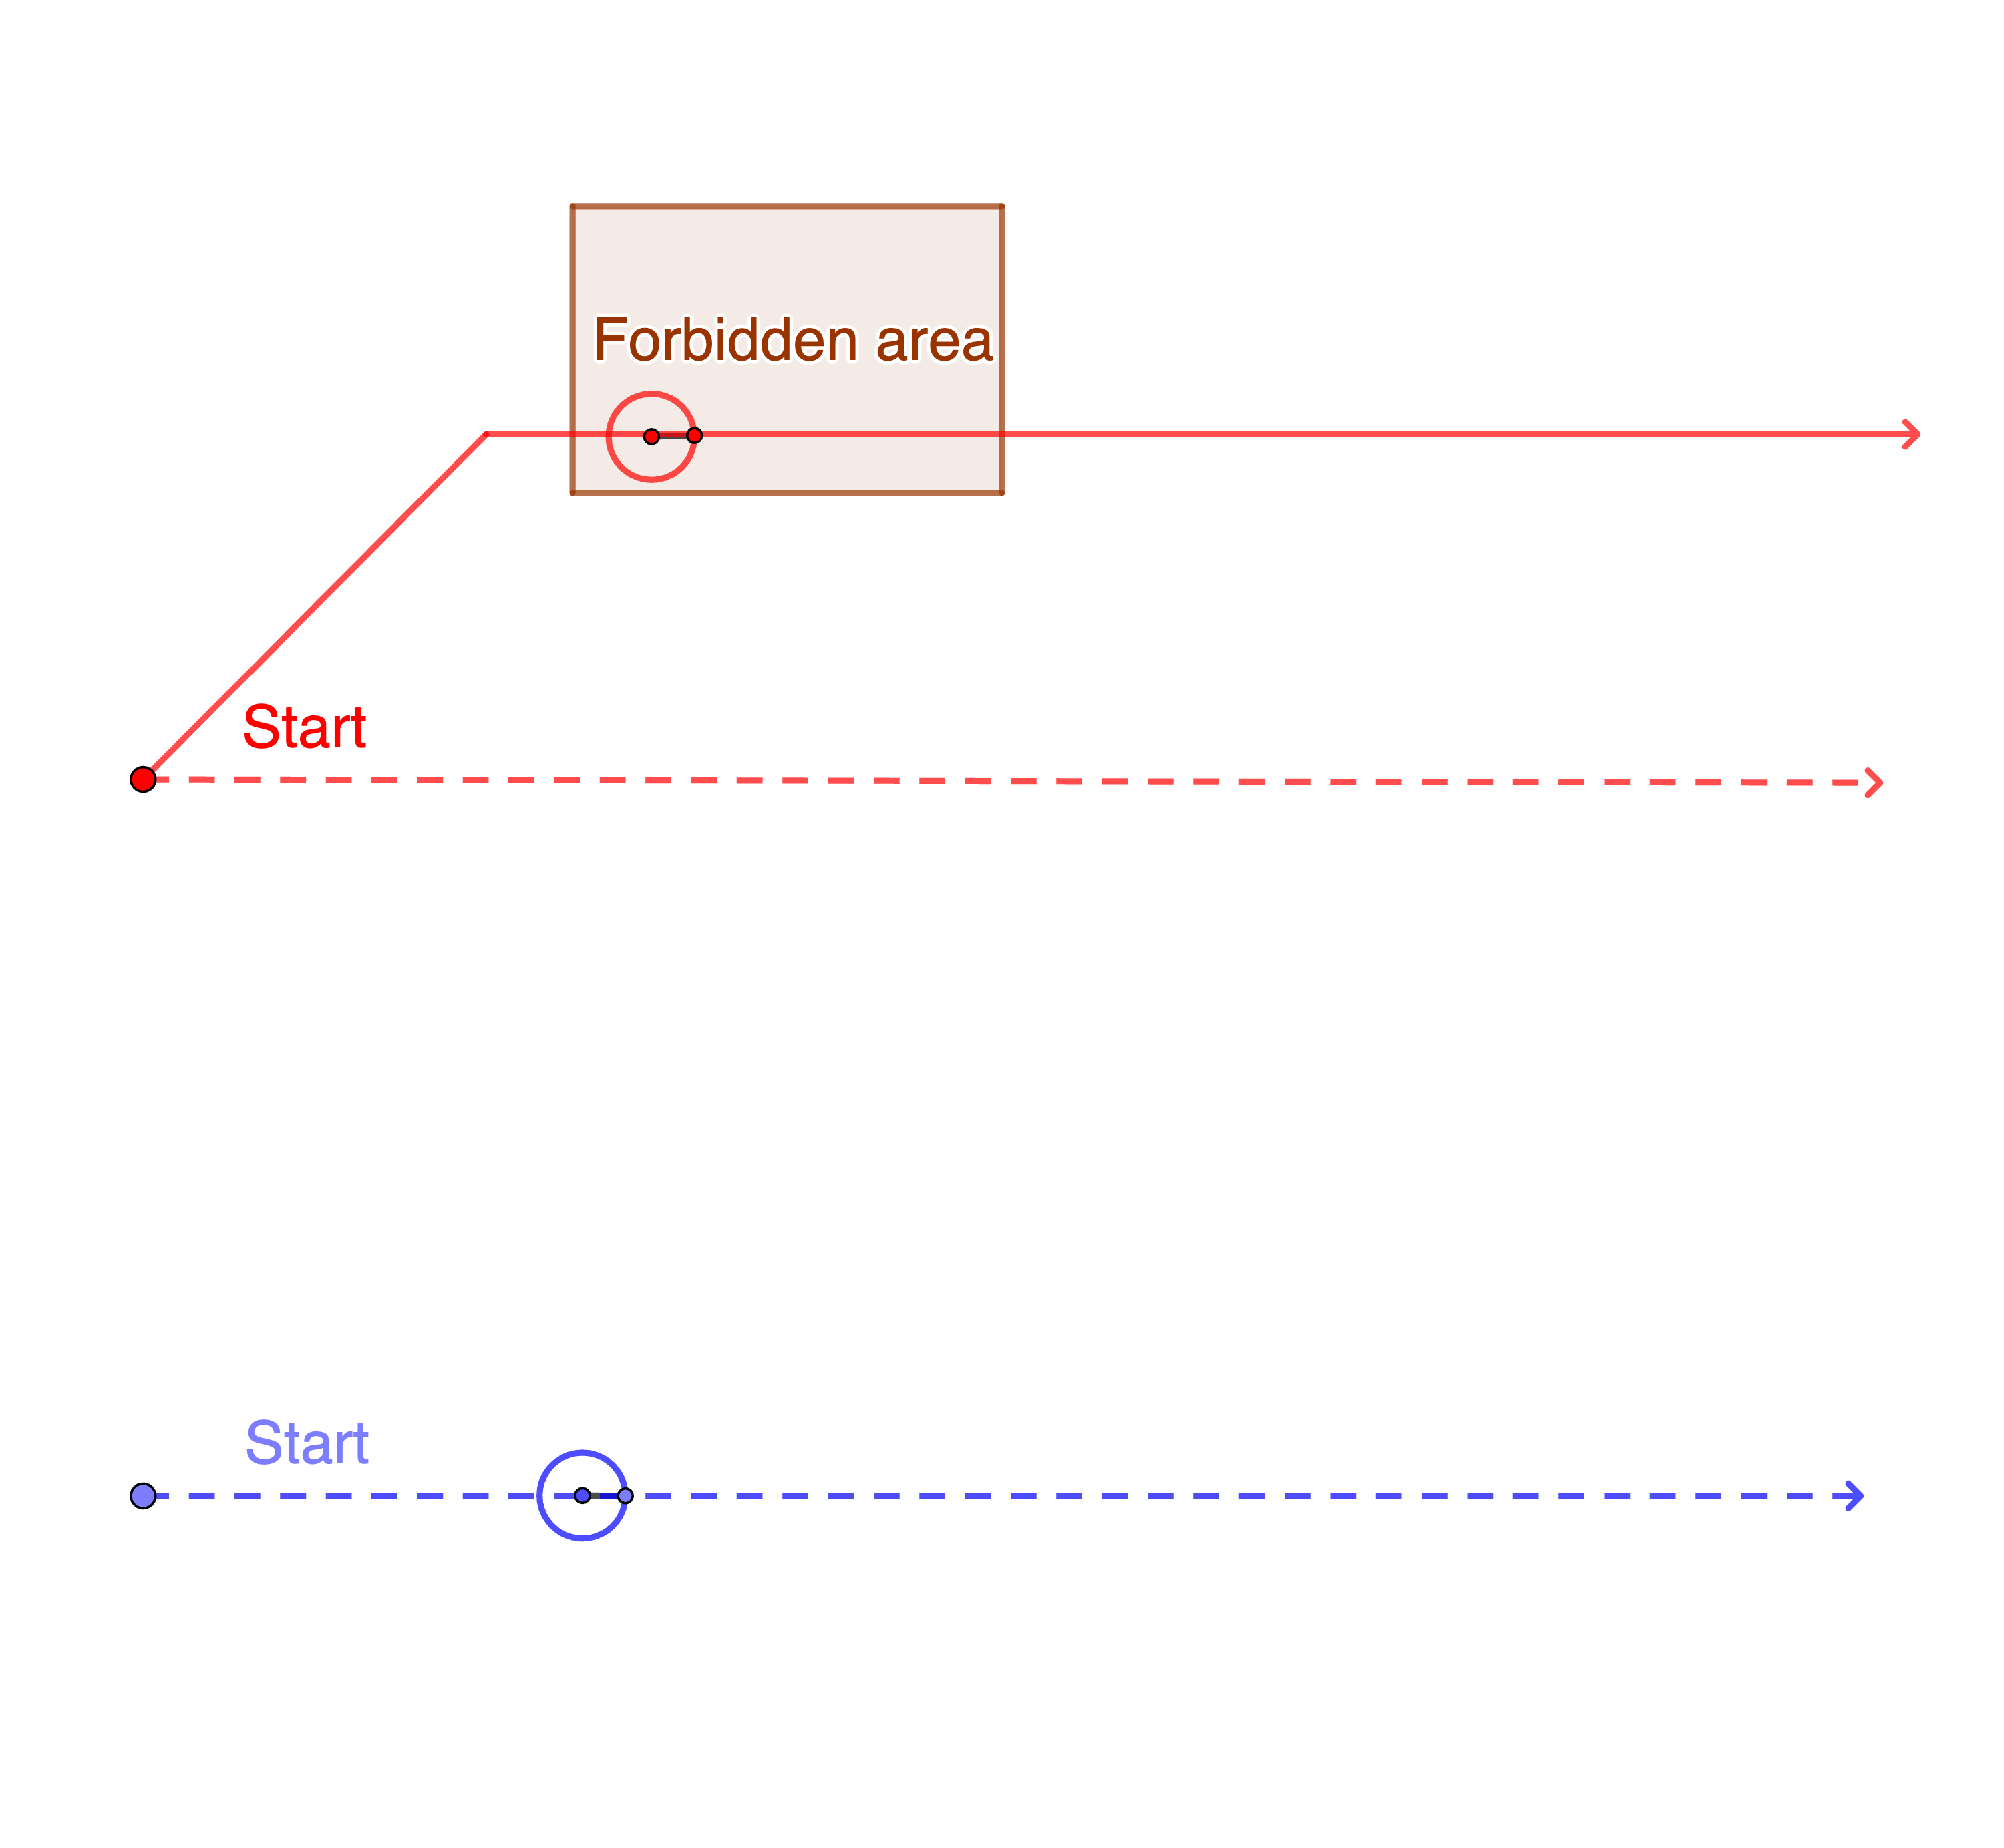
\includegraphics[width = 0.32\linewidth]{plan-deviation}}
    \subfloat[Co-observation \label{fig:example-co-observation}]{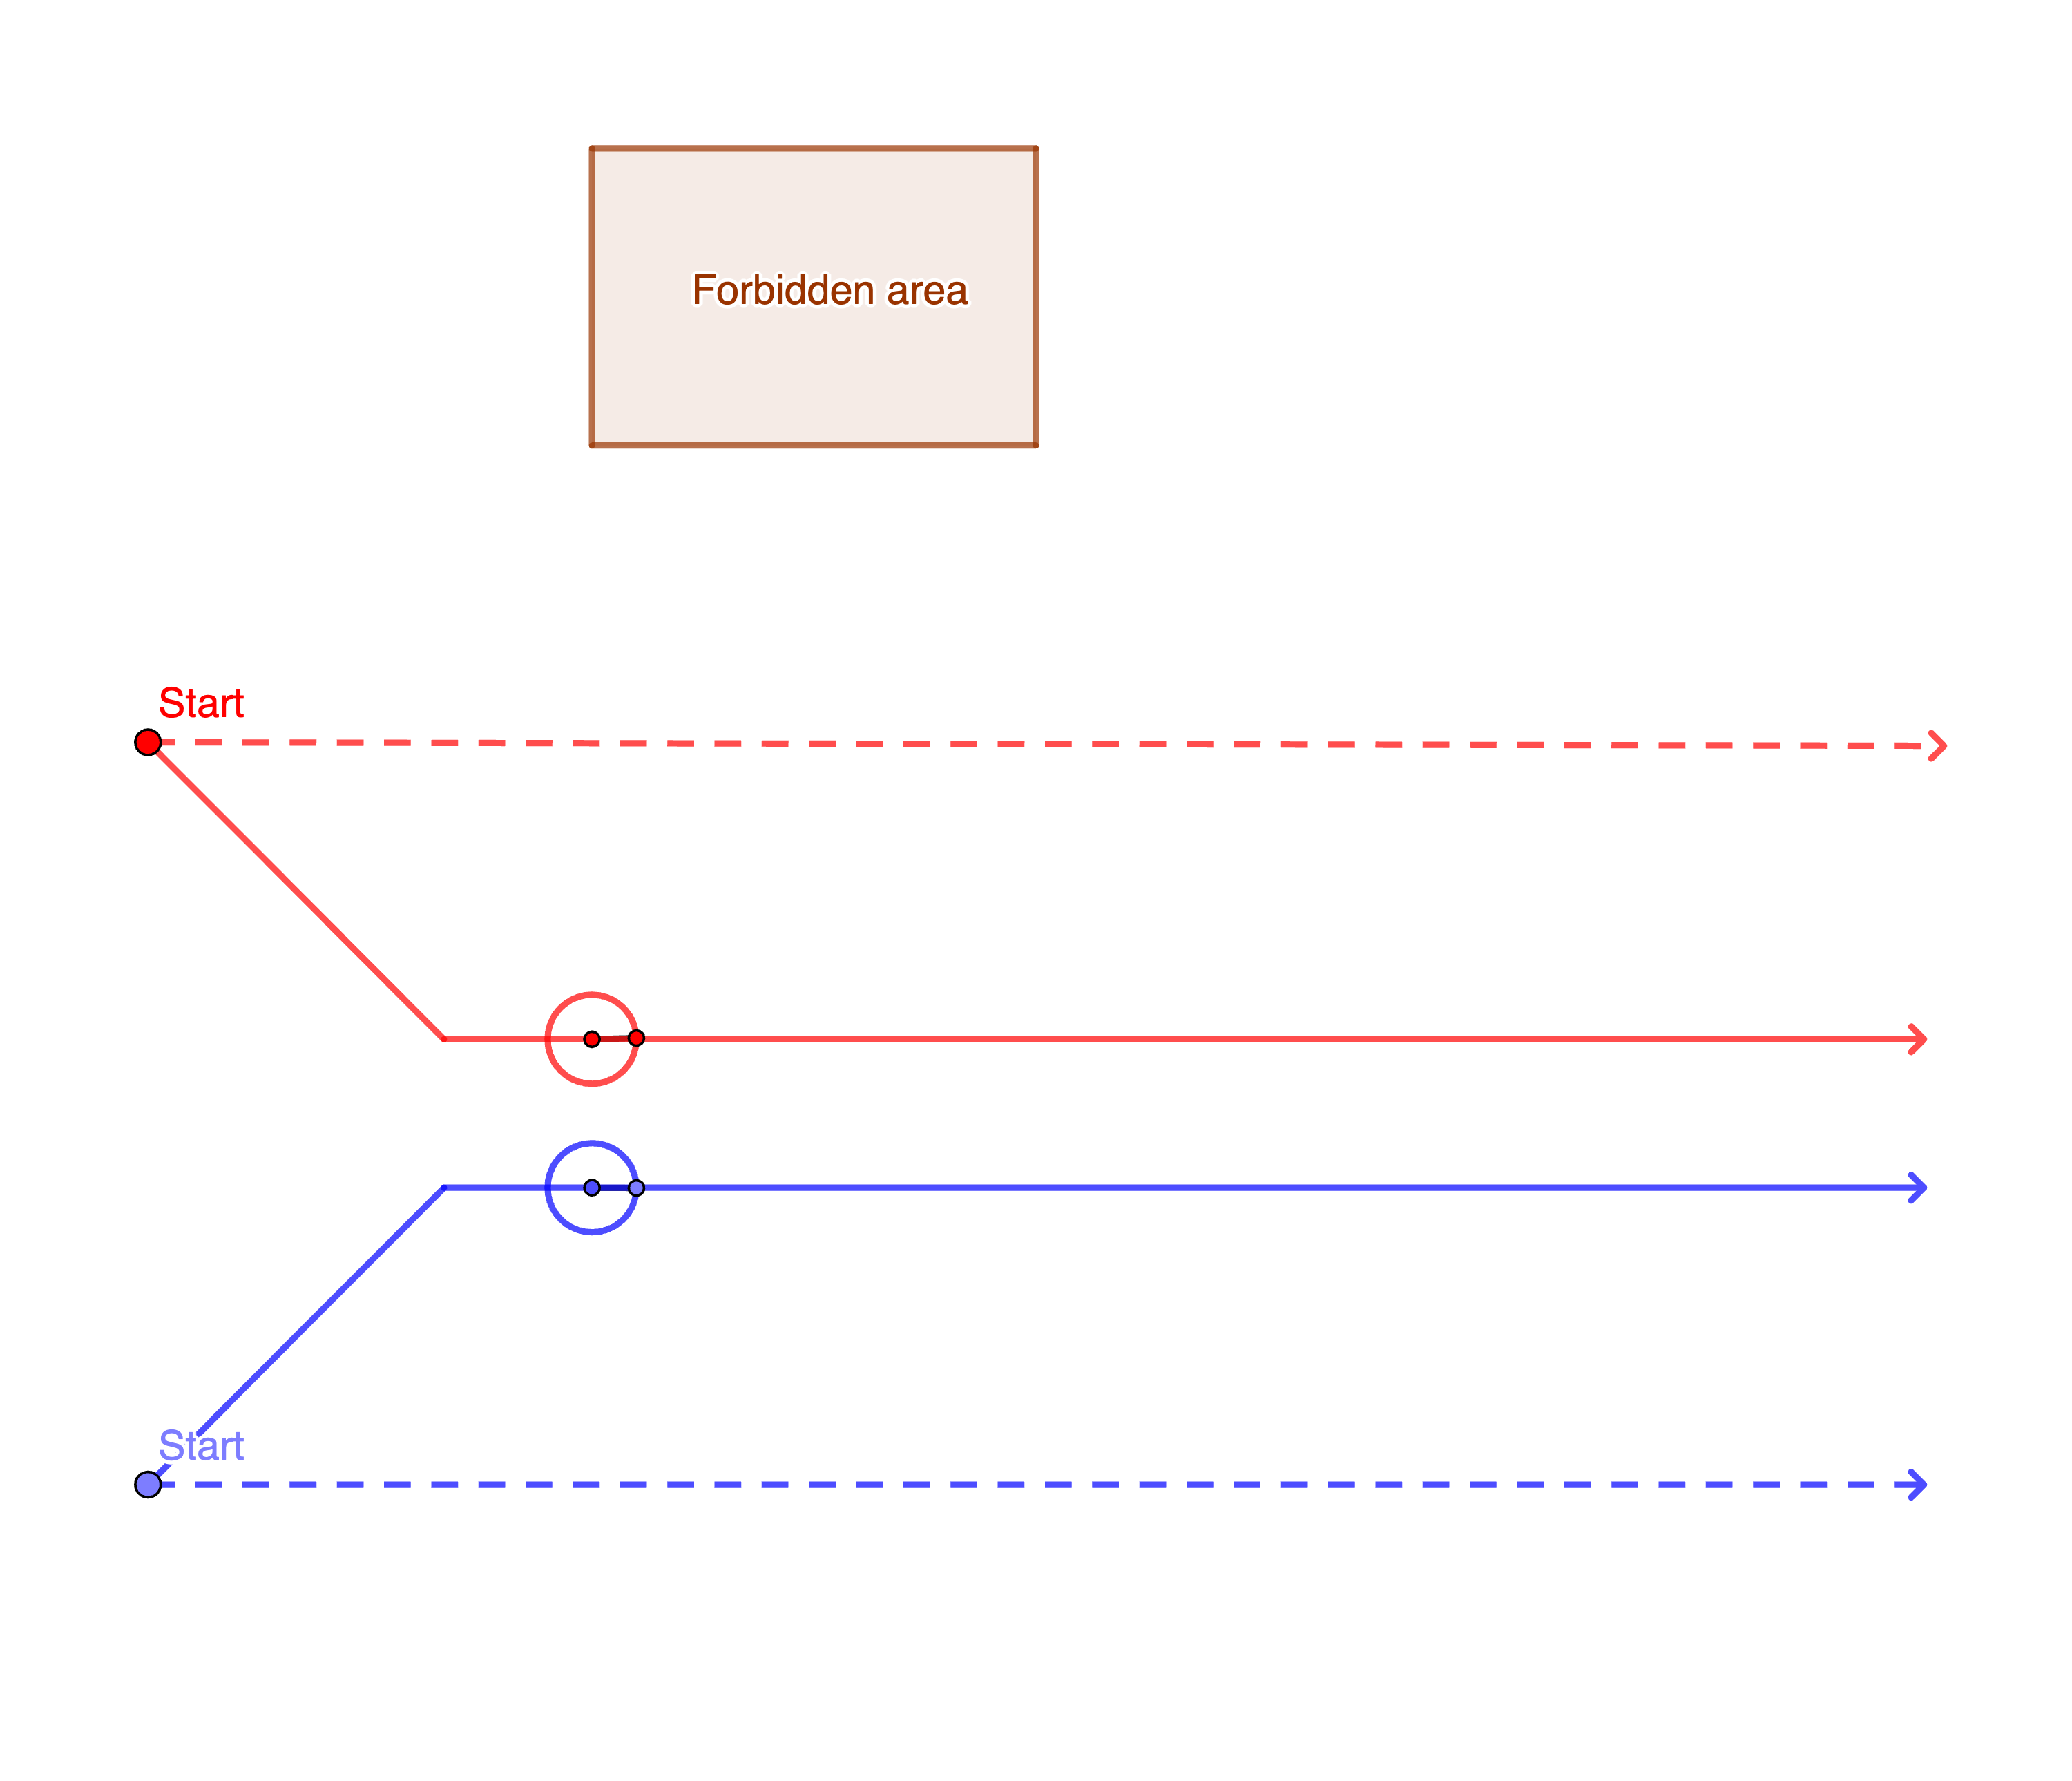
\includegraphics[width=0.32\linewidth]{co-observ}}
    \subfloat[Cross-trajectory co-observation \label{fig:example-cross-traj}]{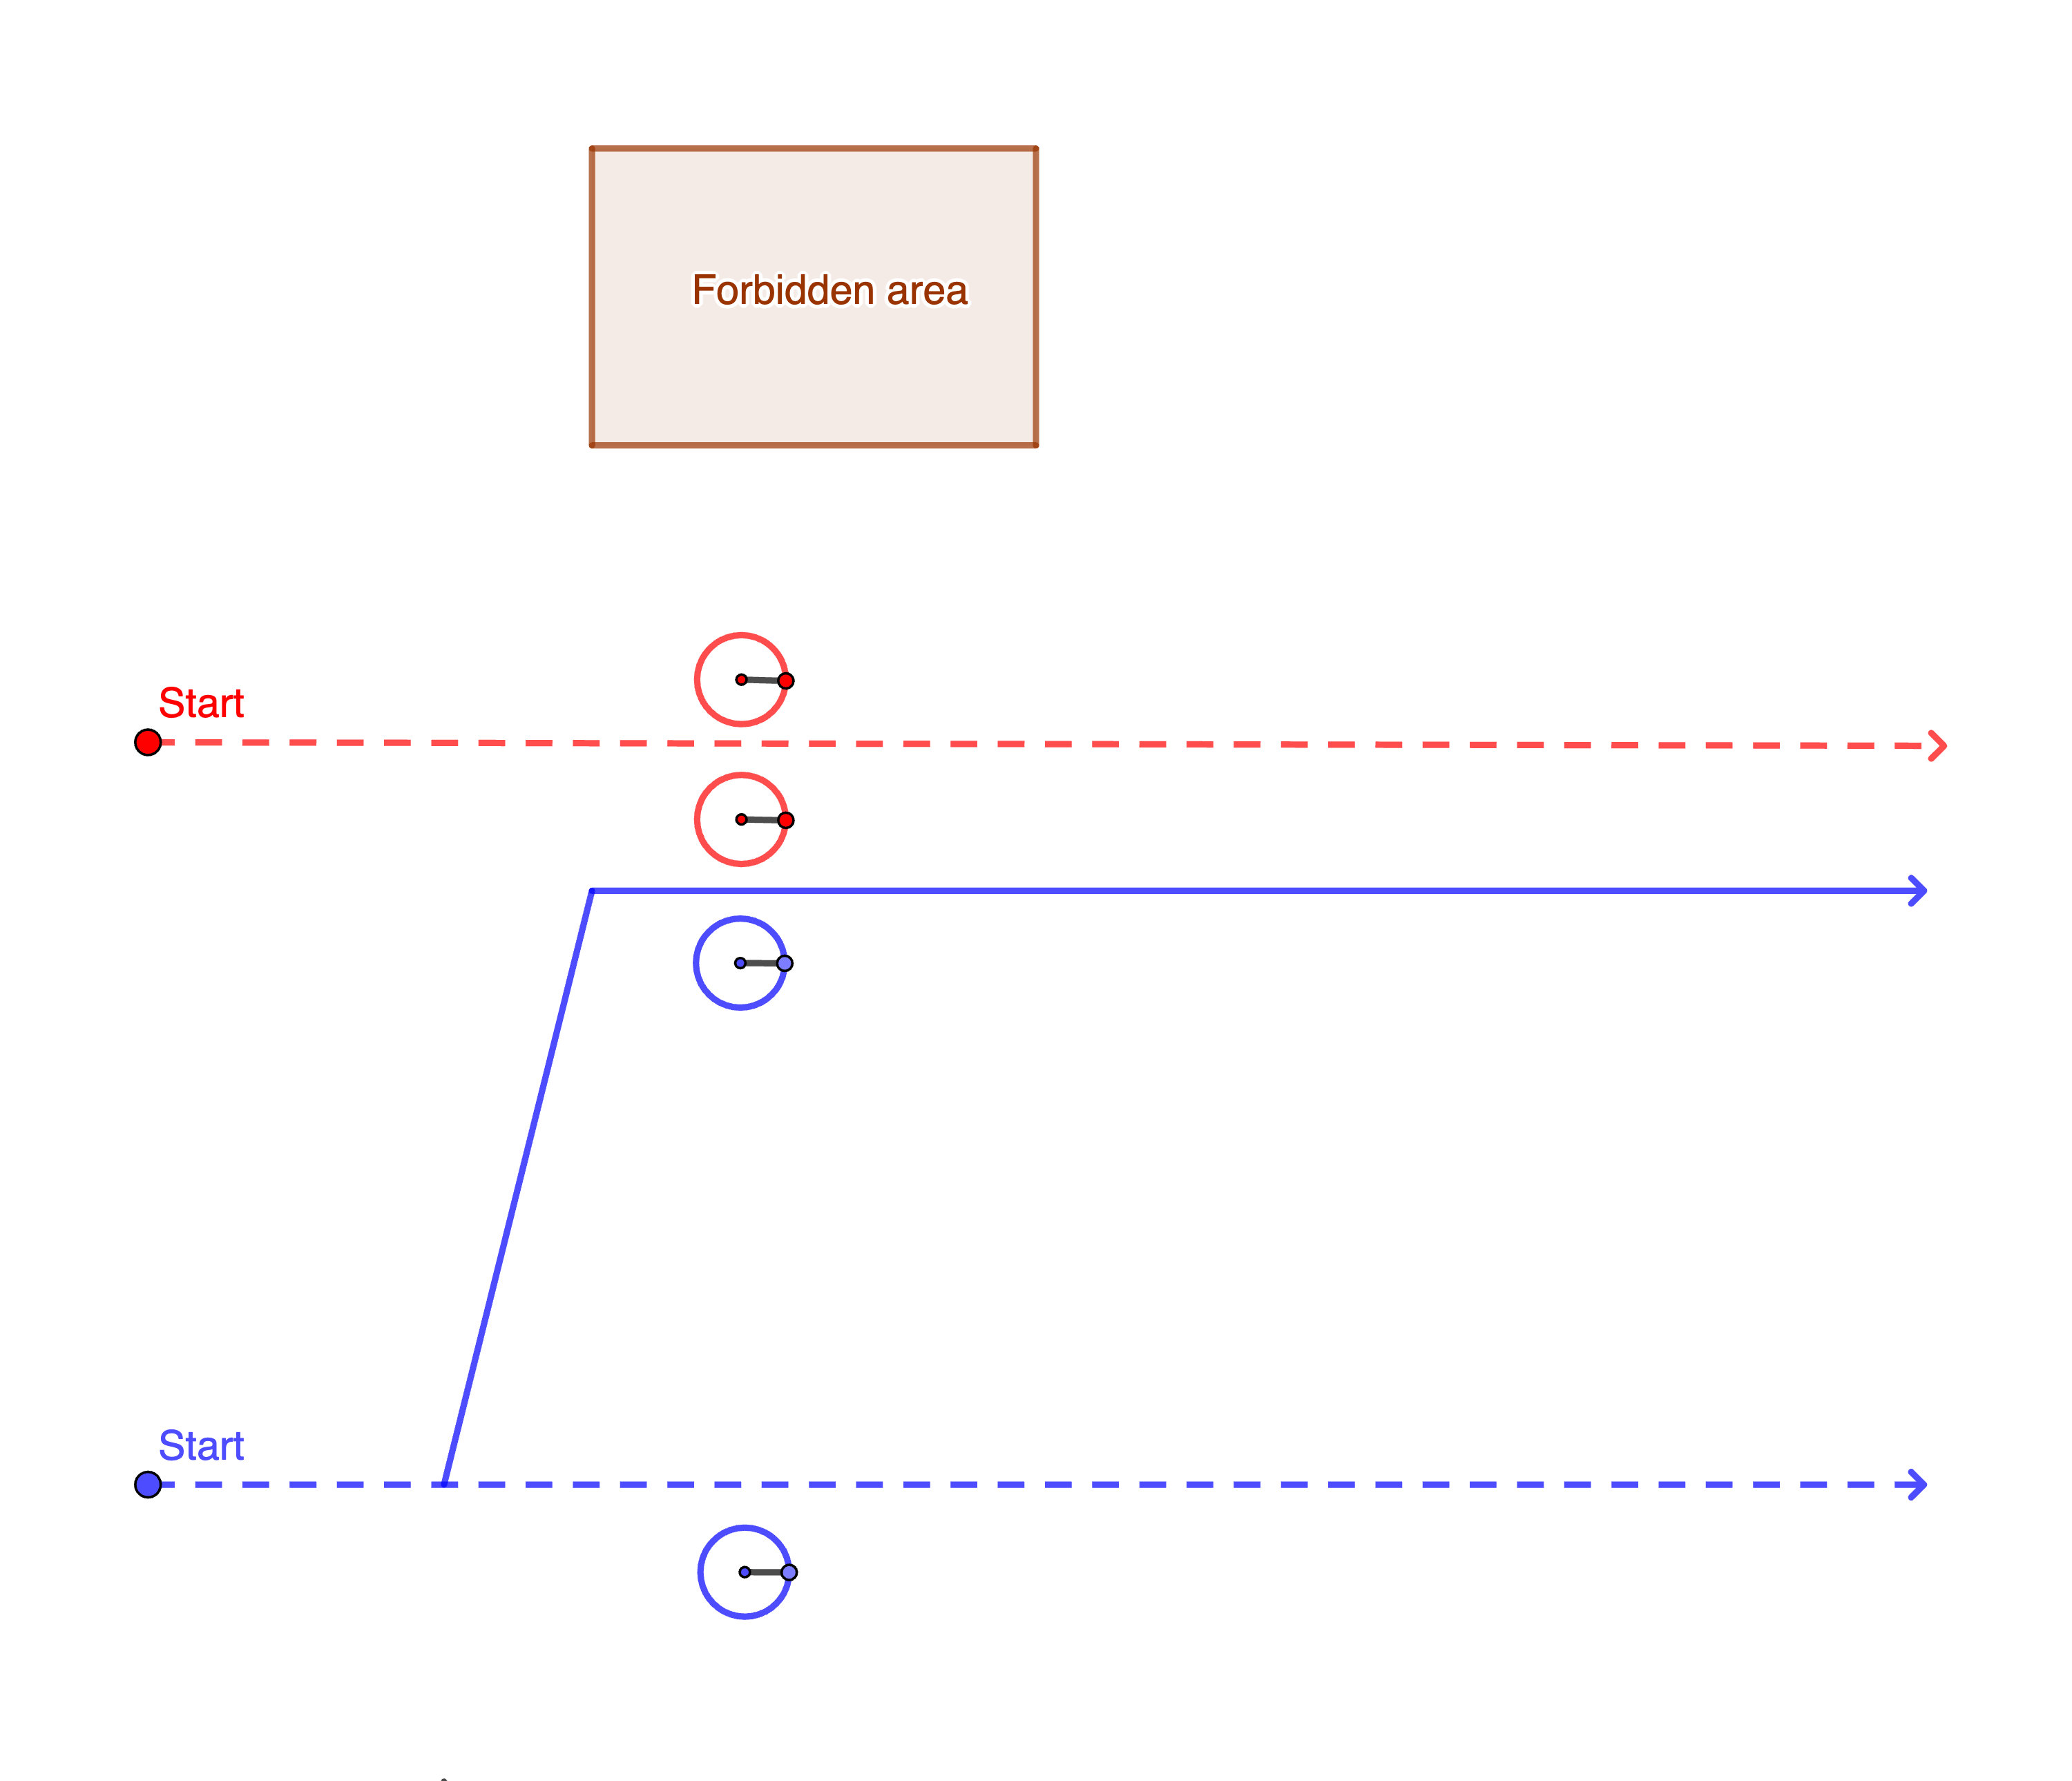
\includegraphics[width=0.32\linewidth]{cross-traj}}
    
    \caption{\ref{fig:example-co-observation} Limited by the co-observation requirement, both red and blue robot follow the co-observation secured routes (solid lines) and abandon the optimal ones (dashed line). \ref{fig:example-cross-traj} Through cross-trajectory co-observations, the blue team sends one robot to follow the red team (solid blue line) and performs co-observation while having the rest of the robots following the optimal trajectory.}\label{fig:cross-traj-comparison-set}
\end{figure}

\paragraph{Paper contributions} In this paper, we formulate a way to enforce an empty intersection between forbidden region and reachability regions, such that if an attacker takes control of the robots, they cannot perform an undetected attack by entering forbidden regions and meeting co-observation schedules at the same time. The constraints are formulated using an ellipsoidal bound of the reachability region. 

We propose to incorporate redundancy in the form of \emph{sub-team}s of multiple robots in place of individual robots along each route. This allows robots to deviate from their assigned sub-team, and join others to perform cross-trajectory co-observations, thereby securing multiple trajectories. We propose a formulation of the multi-flow problem on unsecured MRS trajectories to plan the cross-trajectory co-observations that can preserve the security against plan-deviation attacks.


\section{Multi-robot trajectory planning with co-observation}

In this section, we aim to enhance the security of MRSs against malicious takeovers and deviations by attackers. Specifically, we design an inter-robot observation plan (co-observation schedule) to ensures that, during the task period, robots are constantly in proximity to one another according to a schedule, in order to observe and detect potential hazardous behaviors. 
This achieved by keeping the potential region that the robots can possibly reach between each consecutive co-observations away from the forbidden regions. 
In this way, the plan ensure that any potential deviations to these forbidden regions will cause the corresponding robot to miss their next co-observation with other robots. \cite{wardega2019resilience} solved this problem in grid world for robots with fixed start and goal locations (Figure~\ref{fig:Grid-example-application}) but does not offer the ability to optimize arbitrary smooth cost functions of the trajectories. 

We formulate the planning problem as an optimal trajectory optimization problem to minimize arbitrary smooth objective functions. 
We denote as $q_{ij}\in\real{m}$ the position of agent $i$ at the discrete-time index $j$, with $m$ representing the dimension of the state space. For a team of $n$ agents, and a task time horizon of $T$, the overall trajectory of the multi-agent system can be represented as an aggregated vector $\vq\in \real{n m T}$. 
The goal of our path planning problem is to minimize or maximize an objective function $\varPhi(\vq)$ under a set of nonlinear constraints described by a set $\Omega$. The set $\Omega$ is given by the intersection of spatio-temporal sets given by the security constraints (co-observation schedule, reachability analysis) and the traditional path planning constraints. Formally:
\begin{equation}\label{eq:general-problem}
	\begin{split}
		\min/\max & \quad \varPhi(\vq)\\
		\textrm{subject to} &\quad \vq \in \Omega.
	\end{split}
\end{equation}

To give a concrete example of the cost $\varPhi$ and the set $\Omega$, we introduce a representative application that will be used for all the simulations throughout the paper.

\begin{example} 
We consider the estimation of a slowly-varying scalar or vector field, denoted as $\vx$, at discrete locations within an unknown environment. Autonomous agents navigate this environment, collecting sensory data to construct a corresponding map (see Figure~\ref{fig:ADMM-example-application}). Our map comprises points of interest arranged on a grid, each associated with a slowly-changing value. Our goal is to find paths that minimize uncertainty and effectively reconstruct the field. We utilize Kalman Filters (KFs)~(cf. \cite{anderson2012optimal}) to estimate uncertainty through the covariance $P_j$. Additionally, the robot provides field measurements at waypoints $q$ using a Gaussian radial basis function for radius and quality modeling.

%Assume that there exists a slowly-time-varying scalar or vector field $\vx$ whose value needs to be estimated at a given number of discrete locations. To explore unknown spatially-distributed fields, autonomous agents are usually required to traverse the entire unknown environment while collecting sensory data to estimate a corresponding map (Figure~\ref{fig:ADMM-example-application}). We model the map as a set of locations of interests arranged on a regular grid, where at each location, we assume that there is a corresponding slowly-time-varying quantity. For our purposes, we are interested in finding paths that best reconstruct the field, i.e., that achieve the minimum uncertainty. 

%We address the estimation problem using Kalman Filters (KFs)(cf. \cite{anderson2012optimal}), with a focus on the estimated covariance $P_j$, to calculate the map model uncertainty. We assume the robot provides field measurements at waypoints~$q$, with Gaussian radial basis function modeling radius and quality.
%\rtron{The previous paragraph can be written more compactly.}

Our cost function $\varPhi(\vq)$ measures the maximum uncertainty $P_{j}$ among map locations of interest along the entire trajectory $\vq$, and our objective is to minimize this maximum uncertainty. Constraints $\Omega$ includes traditional constraints like velocity constraints, convex obstacles, waypoints to reach with deadlines, and security constraints including co-observation constraints and reachability constraints.
\end{example}

\begin{figure}
     \centering
     \subfloat[Continuous world trajectory \label{fig:ADMM-example-application}]{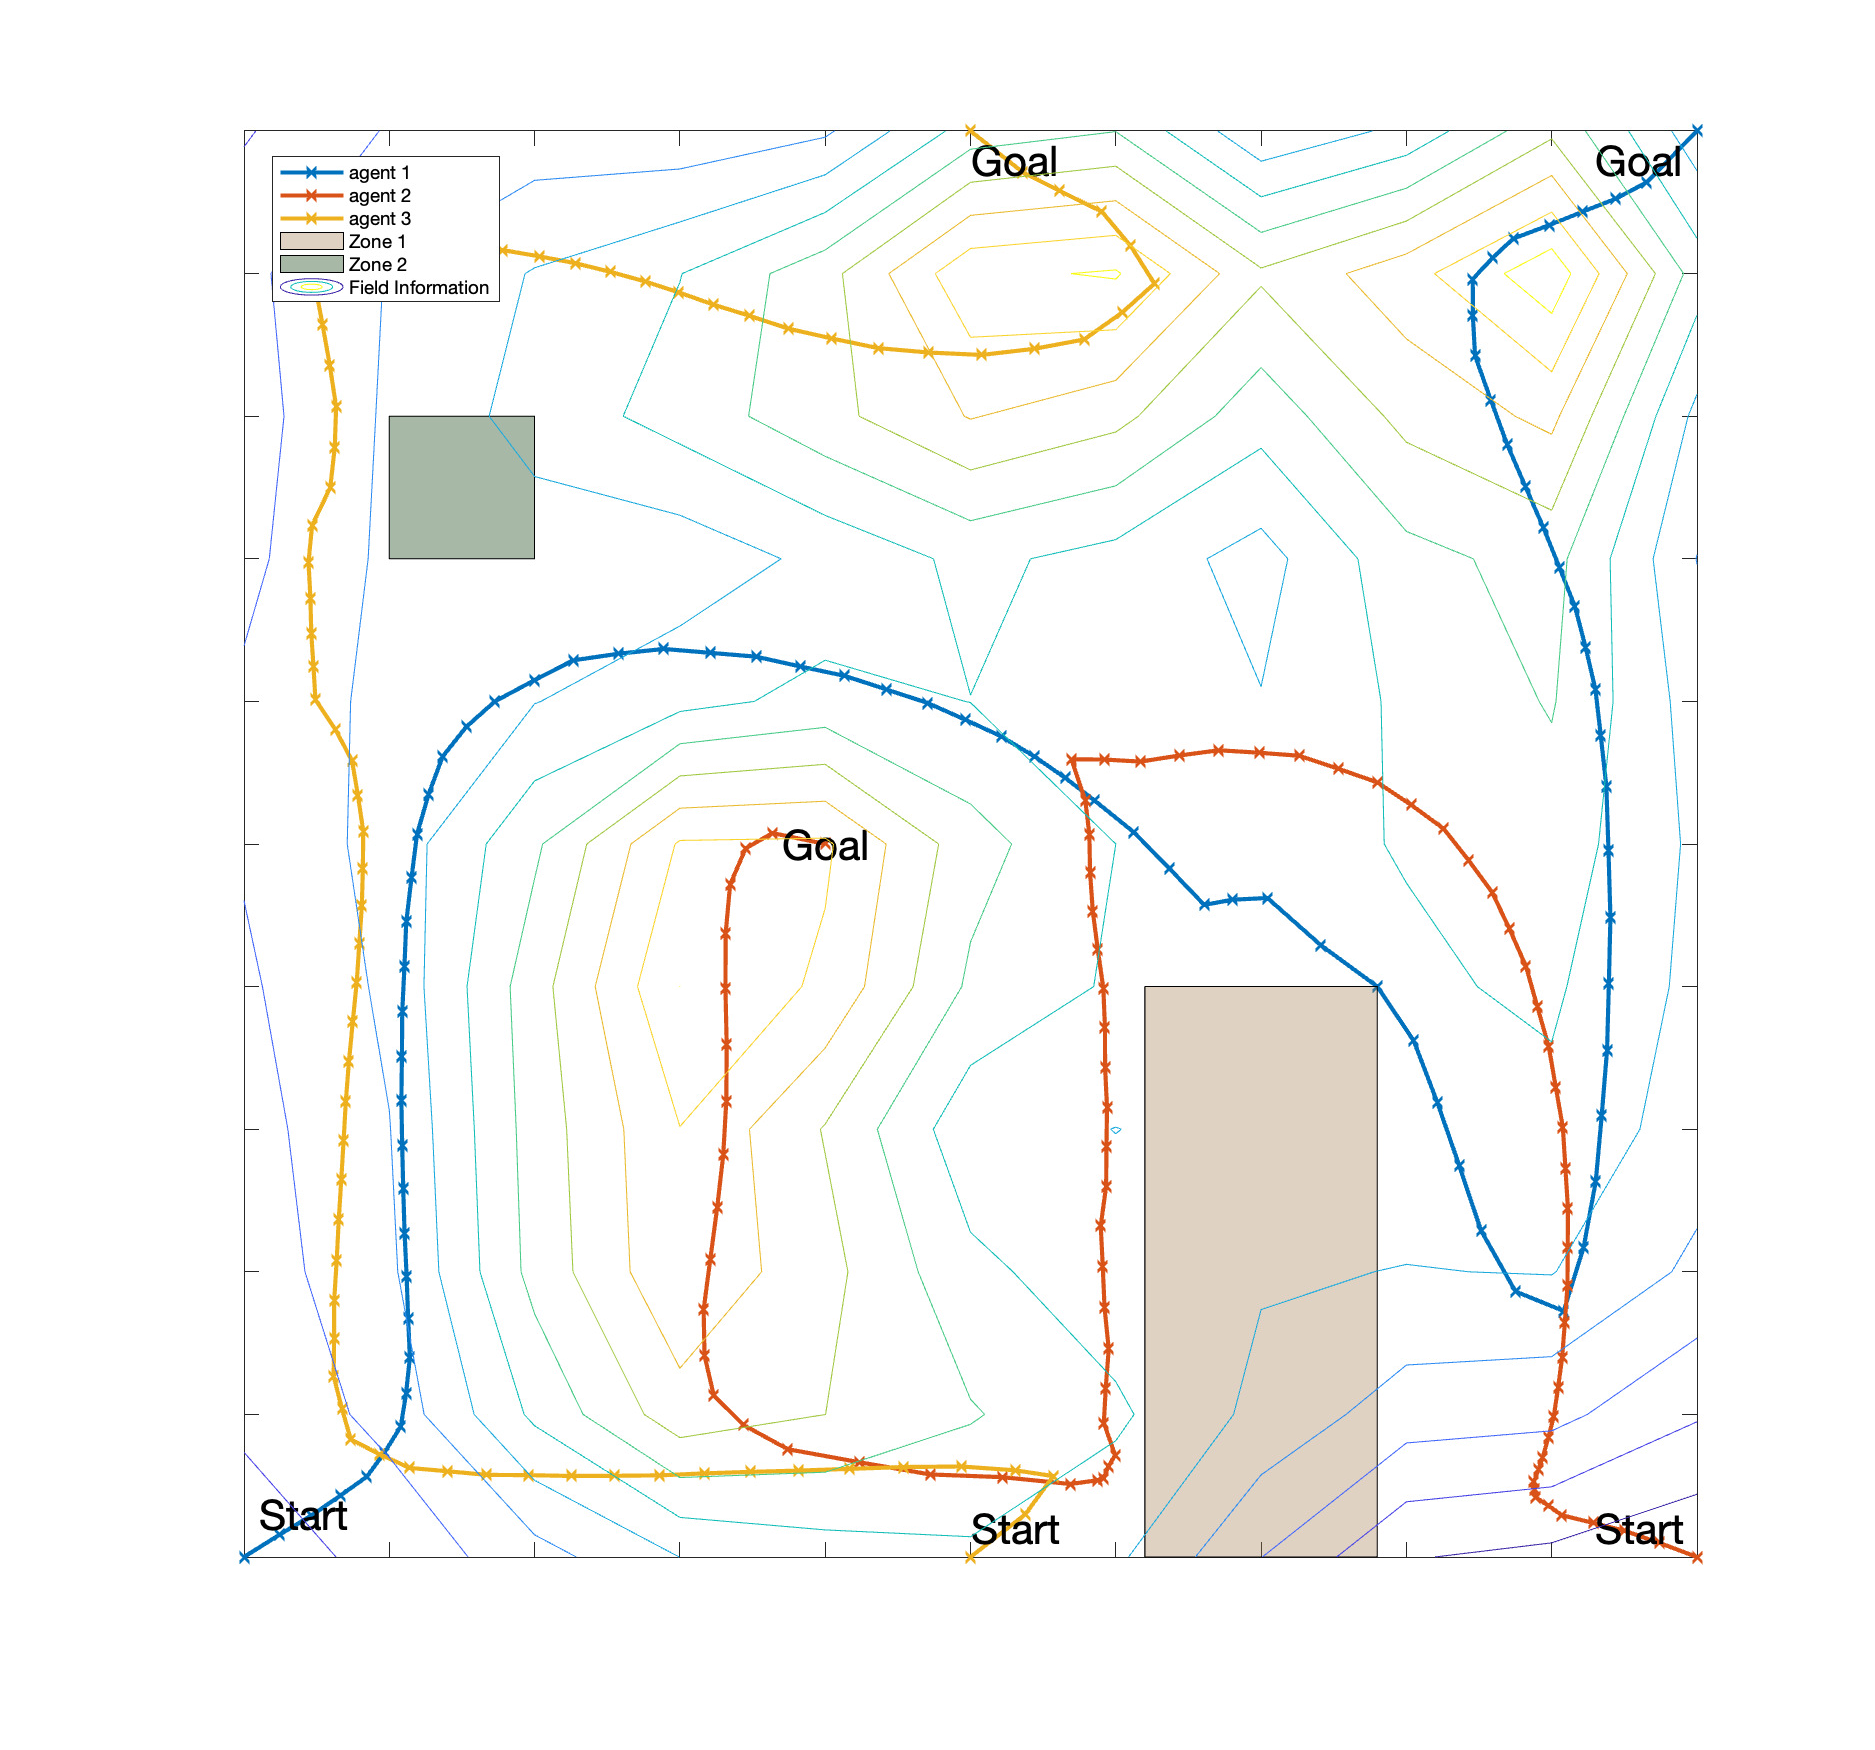
\includegraphics[width=0.45\linewidth, trim = 2cm 2cm 2cm 2cm]{Example_application}}
     \subfloat[Grid-world trajectory. \label{fig:Grid-example-application}]{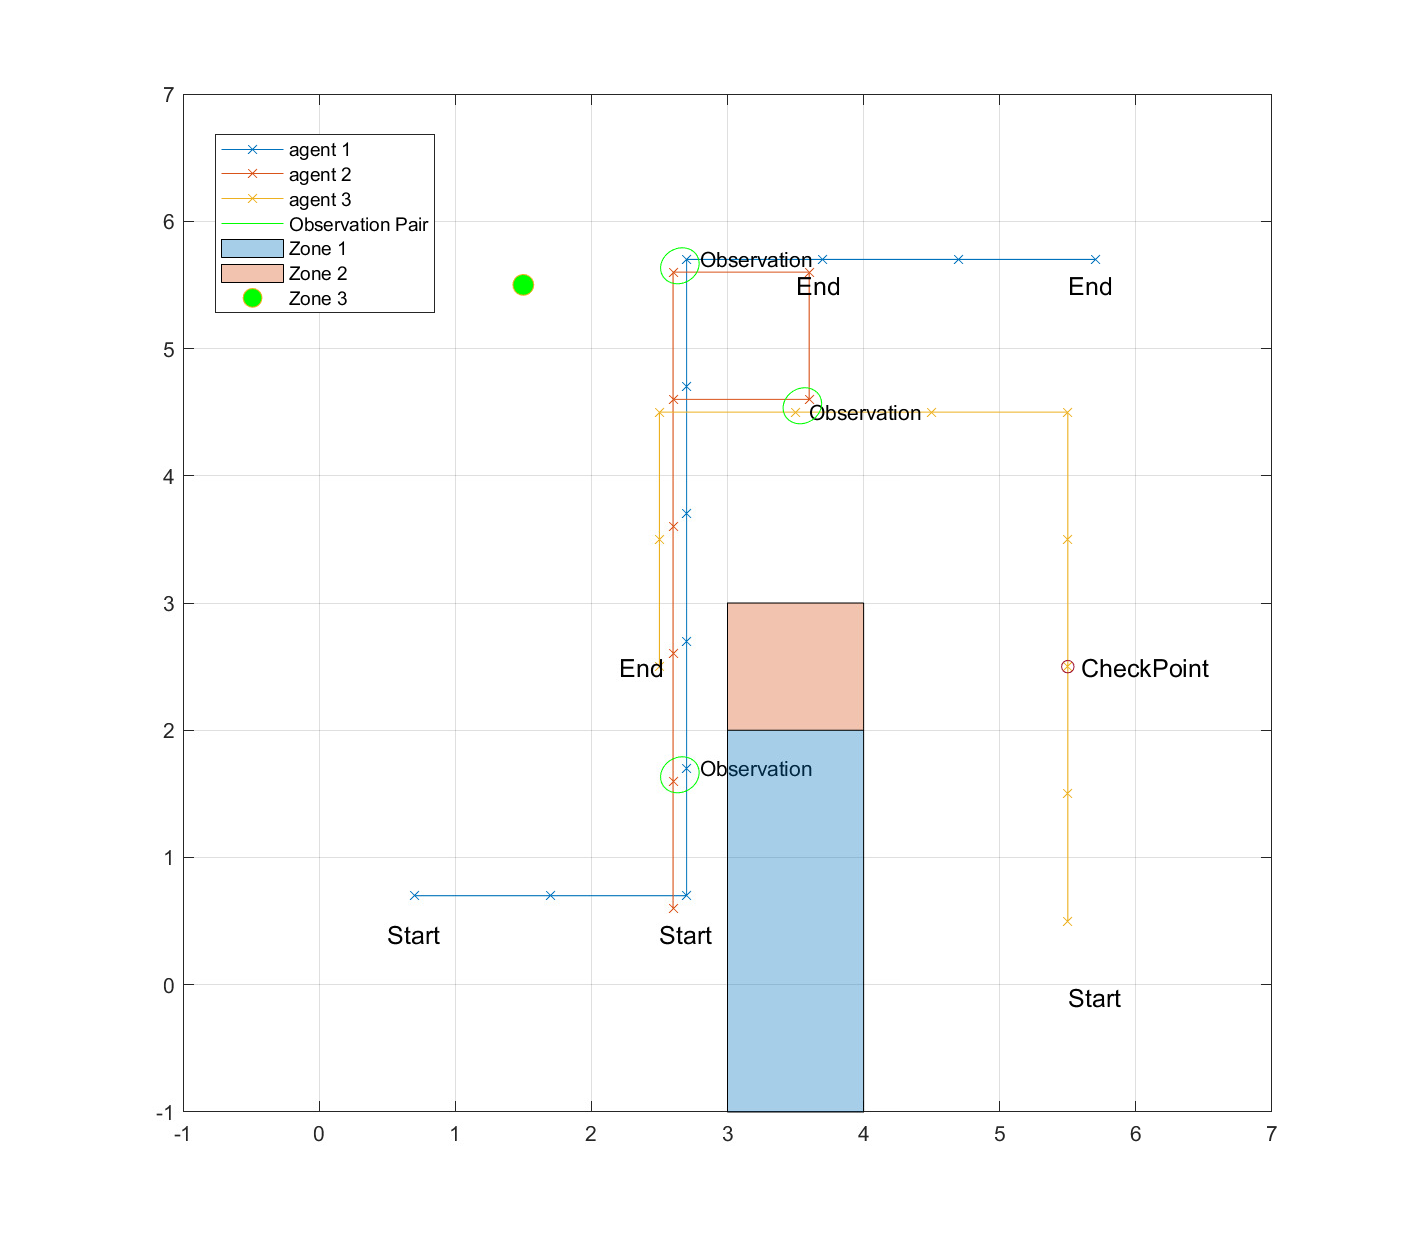
\includegraphics[width=0.45\linewidth, trim = 2cm 0.5cm 0cm 2cm]{Kacper_result}}
     \caption{Trajectory design of an example map exploration task for a three-robot system with start locations and destinations fixed. Task are planned in a $8 \times 8$ grid world. Zone 1 is obstacle, Zone 2 and Zone 3 are safe zones. Fig~\ref{fig:Grid-example-application} shows the planned trajectory with co-observation schedule in grid-world. Fig~\ref{fig:ADMM-example-application} shows the trajectory design in continuous world optimized with respect to a map exploration task}
     \label{fig:example-application}
 \end{figure}
 \rtron{Make sure we refer back to Example 1 when makes sense}
 
 This section is organized as follows. We begin by presenting the foundational mathematical concepts, notably the basic ADMM optimal trajectory solver. Subsequently, our solver allows us to seamlessly integrate security constraints, encompassing co-observation schedule and reachability constraints. Concluding this section, we present the obtained results alongside limitations (due to infeasibility) that are addressed in \Cref{sec:??}.

\subsection{Preliminaries}
In this section, we review various mathematical concepts that will provide the foundations and context for the solver and constraints.

\subsubsection{Differentials}
We define the differential of a map $f(x):\real{m}\to\real{n}$ at a point $x_0$ as the unique matrix $\partial_x f \in\real{n\times m}$ such that
\begin{equation}\label{equ:dt_to_dx}
  \left.\dert f\bigl(x(t)\bigr)\right|_{t=0}=\partial_x f\bigl(x(0)\bigr) \dot{x}(0)
\end{equation}
where $t\mapsto x(t)\in\real{n}$ is a smooth parametric curve such that $x(0)=x$ with any arbitrary tangent $\dot{x}(0)$. For brevity we will use $\dot f$ for $\dert f$ and $\partial_x f$ for $\frac{\partial f}{\partial x}$. The differentials $\partial_x f$ is derived through \eqref{equ:dt_to_dx} having $\dot f$ divided by $\dot x$.

With a slight abuse of notation, we use the same notation $\partial_xf$ for the differential of a matrix-valued function with scalar arguments $f:\real{R}\to\real{m\times n}$.  Note that in this case \eqref{equ:dt_to_dx} is still formally correct, although the RHS needs to interpret $\partial_x f$ as a linear operator applied to $\dot{x}$.

 \subsubsection{Householder rotations}\label{sec:householder}
 In the derivation of the reachability constraint in \Cref{sec:??}, we need to define a differentiable transformation to a canonical form. This transformation will include a rotation that we derive from a modified version of Householder transformations \cite{householder1958unitary}. With respect to the standard definition, our modification ensures that the final operator is a proper rotation (i.e., not a reflection). We call our version of the operator a \emph{Householder rotation}. In this section we derive Householder rotations and their differentials for the 3-D case; the 2-D case can be easily obtained by embedding it in the $z=0$ plane.

  \begin{definition} Let $\nu_\cF$ and $\nu_\cE$ be two unitary vectors ($\norm{\nu_\cF}=\norm{\nu_\cE}=1$). Define the normalized vector $u$ as
    \begin{equation}
      u'=\nu_\cF+\nu_\cE,\quad u =\frac{u'}{\norm{u'}}.
    \end{equation}
    The \emph{Householder rotation} $H(\nu_\cF,\nu_\cE)$ is defined as
    \begin{equation}\label{eq:H definition}
      H(\nu_\cF,\nu_\cE) = 2 u u\transpose-I.
    \end{equation}
  \end{definition}
  The main property of interest for our application is the fact that $H$ is a rotation mapping $\hat{\nu_\cF}$ to $\hat{\nu_\cE}$, as shown by the following.
  \begin{proposition}\label{prop:HProperty}
    The matrix $H$ has the following properties:
    \begin{enumerate}
    \item It is a rotation, i.e.
      \begin{enumerate}
      \item\label{it:orthonormality} $H\transpose H=I$;
      \item\label{it:determinant} $\det(H)=1$.
      \end{enumerate}
    \item\label{it:transformation} $\nu_\cE=H \nu_\cF$.
    \end{enumerate}
  \end{proposition}
  \begin{proof}
  	See Appendix \ref{proof:HProperty}.
  \end{proof}

  We compute the differential of $H$ implicitly using the relation \eqref{equ:dt_to_dx}. We will use the notation $\cross{v}:\real{3}\to\real{3\times 3}$ to denote the matrix representation of the cross product with the vector $v$, i.e.,
  \begin{equation}
    \bmat{v_1\\v_2\\v_3}\mapsto \bmat{0 & -v_3 &v_2\\v_3 & 0 & -v_1\\-v_2 & v_1 & 0},
  \end{equation}
  such that $[v]_\times w=v\times w$ for any $w\in\real{3}$. %One can verify by direct computation the following property:
  %\begin{equation}\label{eq:asymmetric to cross}
  %  wv\transpose-vw\transpose=\cross{\cross{v}w}.
  %\end{equation}
  \begin{proposition}\label{prop:Hderivitive}
    Let $\nu_\cF(t)$ represent a parametric curve. Then we have
    \begin{equation}
      \dot{H}=H\cross{-2M\dot{\nu}_{\cF}}
    \end{equation}
    where the matrix $M\in\real{3\times3}$ is given by
    \begin{equation}
      M=[u]_{\times}  \frac{ \left( I - u u\transpose \right) \left( I- \nu_\cF \nu_\cF\transpose \right)} {\norm{u'} \norm{\nu_\cF}}.
    \end{equation}
  \end{proposition}
  \begin{proof}
  	See Appendix \ref{proof:Hderivitive}.
  \end{proof}

\subsubsection{Alternating Directions Method of Multipliers (ADMM)}\label{chapter:ADMM review}
The basic idea behind our ADMM-based solver \cite{zyang} is to split the constraints from the objective function using a different set of variables $\vz$, and then solve an Augmented Lagrangian formulation of the optimization problem in \eqref{eq:general-problem}.
More specifically, we can rewrite the constraint $\vq\in\varOmega$ using an indicator function $\varTheta$, and include it in the objective function. In the traditional application of ADMM, the variables $\vz$ are duplicates of $\vx$ projected to the constraint set $\Omega$. However, in path planning problems, some constraints are non-convex, rendering the projection step more difficult (due to the presence of multiple local minima).
To allow for a easier projection step, we propose a minor generalization of the ADMM formulation where we allow $\vz$ to replicate an arbitrary function of the main variables $\vq$ (instead of being an exact copy), to transform constraint $\vq\in\Omega$ to $D(\vq) \in \sZ$ : 
\begin{equation}\label{eq:ADMMSetConstraint_modified}
	\begin{aligned}
		&\max\quad \varPhi(\vq)+\varTheta(\vz) \\
		& \begin{array}{r@{\quad}c}
			s.t.& D(\vq)-\vz=0
		\end{array} 
	\end{aligned}
\end{equation}
where $D(\vq)= [D_1(\vq)^T,\dots,D_l(\vq)^T]^T$ is a vertical concatenation of different functions for different constraints.

The update steps of the ADMM algorithm can be then denoted as \cite{Boyd2011}:
\begin{subequations}\label{eq:ADMMupdate}
	\begin{align}
		\label{eq:admm-mod-update-q}\vq^{k+1}&:=\argmin_\vq(\varPhi(\vq^k) +\frac{\rho}{2}\norm{D(\vq)-\vz^k+\vu^k}_2^2)\\
		\vz^{k+1}&:=\Pi_\mathcal{Z}(D(\vq^{k+1})+\vu^k) \\
		\vu^{k+1}&:=\vu^k+D(\vq^{k+1})-\vz^{k+1},
	\end{align}
\end{subequations}
where $\Pi_\mathcal{Z}$ is the new projection to the modified constraint set $\mathcal{Z}$, $\vu$ represents a scaled dual variable that, intuitively, accumulates the sum of primal residuals
\begin{equation}\label{eq:primal-residual}
	\vr^{k}=D(\vq^{k+1})-\vz^{k+1}.
\end{equation}
Checking the primal residuals alongside with the dual residuals 
\begin{equation}\label{eq:dual-residual}
	\vs^{k}=-\rho(\vz^{k}-\vz^{k-1}),
\end{equation}
after each iteration, the steps are reiterated until convergence when the primal and dual residuals are small, or divergence when primal and dual residual remains large after a fixed large number of iterations.
Since $D(\vq)$ is the vertical concatenation of $D_i(\vq)$, the projection of each set $\mathcal{Z}_i$ is independent for each constraint and can be computed separately. The advantage of this formulation is that we can choose $D(\vq)$ such that the new constraint set~$\cZ$ becomes simple to compute; however, the drawback is that we move the non-convexity to the primal cost function, i.e., in the update for $\vq$ in \eqref{eq:admm-mod-update-q}.
Additionally, the function~$D(\vq)$ can be used to select only the subset of the variables on which a constraint depends, speeding up computations.

We now provide the functions $D(\vq)$, the sets $\cZ$, and the corresponding projection operators $\Pi_\cZ$ for traditional path planning constraints (\Cref{sec:velocity-constraint}-\Cref{sec:waypoint-constraint}), co-observation security constraints (\Cref{sec:co-observation-constraint}), and reachability constraints (\Cref{sec:ellipsoid-point}-\Cref{eq:region_ellipsoid_constraint}). The latter are based on the definition of \emph{ellipse-region-constraint} (\Cref{sec:reachability}).

\subsection{Velocity constraints}\label{sec:velocity-constraint}
  The movement of each agent is constrained by a maximum distance in any direction over a single discrete time step. We then define the function $D(\vq)$ to return the velocity vectors for the $i$-th agent at time step $j$; its result then needs to be constrained to a sphere.

  \begin{constraint}[Velocity constraint]
\begin{align}
     D_{ij}(\vq) &= q_{ij}-q_{i(j-1)}, \quad j\in\{1,\ldots, T\}\\
\label{eq:velocity_constraint}
   \sZ_{ij} &=\bigl\{\vz \mid \norm{\vz} \leq v_{max}\bigr\}\\
   \Pi_{\sZ_{ij}}(\vz)&=\begin{cases}
   v_{\max}\frac{\vz}{\norm{\vz}} \textrm{ if } \norm{\vz}>v_{\max}\\
   \vz\textrm{ otherwise}
   \end{cases}
\end{align}
\end{constraint}

\subsection{Convex polygonal obstacles collision constraints} \label{sec:obstacle-constraint}

We use convex polygons to model regions defining solid obstacles and forbidden regions that cannot be entered by agents. The convex region $\cP$ is defined using a collection of $l$ hyperplanes $n_{k} q = m_{k}$, where $n_k$ is the normal vector pointing toward the outside of the obstacle and $m_k$ is the scalar offset defining the $k$-th hyperplane. The distance between a single waypoint $q_{ij}$ and the $k$th hyperplane $d_{k}(q_{ij},\cP)$ is defined as:
\begin{equation}
    d_{k}(q_{ij},\cP)= p_{ij}\transpose n_k - m_k.
\end{equation}
We then defined function $D(\vq)$ to return the maximum distance from $q_{ij}$ to all hyperplane boundaries of region $\cP$, and set constraint on $z$ that it is a non-negative scalar. This constraint is applied to all $q_{ij} \in \vq$. 

\begin{constraint}[Obstacle constraint]
\begin{align}
     	D(q_{ij}) &= \max_{k=1,\dots,l} (d_{k}(q_{ij},\cP))\\
\label{eq:obstacle_constraint}
  \sZ &= \{z \mid z \geq 0 \},\\
   \Pi_\sZ(z) & = \begin{cases}
   0 & \textrm{if} \quad z < 0\\
   z  & \textrm{otherwise}
   \end{cases} \label{eq:zoneConstraintProjection}
\end{align}
\end{constraint}

The motivating idea for \eqref{eq:obstacle_constraint} and \eqref{eq:zoneConstraintProjection} is to identify waypoints within a specific region and project them to the closest boundary. Non-convex obstacles can be handled by the union of (possibly overlapping) convex obstacles. By setting the normal vector pointing toward the inside of the region, this method can also serve to constrain the robots within the designated workspace region.

\subsection{Waypoints with flexible deadlines}\label{sec:waypoint-constraint}
Security-related constraints often necessitate that a robot reaches a specified location at a particular time. We assume robot $i$ is tasked with reaching a given point $p$ within a radius of $d_{max}$ at some time instant $j$ within a predefined time window $[t_1,t_2]$. We defined a constraint this constraint as follow.

\begin{constraint}[Waypoint constraint]
\begin{align}
     	D(\vq) &= \min_{j\in\{t_1,\dots,t_2-1\}}\bigl(\dist(p,\overrightarrow{q_{ij}q_{i(j+1)}})\bigr)\\
\label{eq:waypoint_constraint}
  \sZ &= \{z \mid z < z_{max} \},\\
   \Pi_\sZ(z) & = \min(z, d_{max}).
\end{align}
\end{constraint}

where $\dist(p,\overrightarrow{q_{ij}q_{i(j+1)}})$ returns the distance between the fixed point $p$ and the segment $\overrightarrow{q_{ij}q_{i(j+1)}}$. Note that this function returns the smallest distance between $(p,q_{ij})$ and $(p,q_{i(j+1)})$ if the projection of the point $p$ does not lie on the line segment~$\overrightarrow{q_{ij}q_{i(j+1)}}$; as a consequence, this constraint does not need to be satisfied exactly at one of the points on the discretized trajectory, but it can also be satisfied ``en route'' on the segment between them.
\rtron{Give example application here, and include application of ADMM without the security constraints, but highlighting a path that would break the security}
\zyang{plot new simpler example, add collision avoidance}

%\subsection{Secure Multi-robot path planning using co-observation and reachability constraints}
\subsection{Co-observation schedule constraint}\label{sec:co-observation-constraint}
The co-observation constraint ensures that two robots come into close proximity at scheduled times to observe each other's behavior. This constraint is represented as a relative distance requirement between the two robots at a specific time instant, ensuring they are within a defined radius to inspect each other or exchange data. Importantly, the co-observation locations must be chosen to guarantee that the ellipsoidal reachability regions, as discussed in \Cref{sec:reachability}, do not intersect with any forbidden regions.

%The co-observation constraints is used to guarantee that, at time required by the schedule, two robots should get close enough with each other to observe each other's behavior. This constraint is modeled as a relative distance constraint between two robots at some time instant $j$ (i.e., to require two agents see each other within a certain radius to inspect each other, or to exchange data). The location of the co-observation should make sure that the ellipsoidal reachability region between each co-observation, considered in later sections \ref{sec:reachability}, has an empty intersection with all forbidden regions.

 We write the function for the constraint as:
\begin{constraint}[Co-observation constraint]
\begin{align}
D(\vq) &= \overrightarrow{q_{aj}q_{bj}}, \label{eq:waypoint_constraint}\\
  \sZ &= \{\vz \mid \norm{\vz} \leq d_{max} \},\\
   \Pi_\sZ(z) & = \begin{cases}
d_{max}\frac{\vz}{\norm{\vz}} &\text{if } \norm{\vz} > d_{max},\\
\vz	& otherwise.
\end{cases}
\end{align}
\end{constraint}

where $a,b$ are the indices of the pair of agents required for a mutual inspection. The locations $q_{aj}$ and $q_{bj}$ where the co-observation performed are computed as part of the optimization.

\subsection{Definition of ellipsoidal reachability regions}\label{sec:reachability}
  In this section, we define  \emph{ellipsoidal reachability regions} based on pairs of locations on a trajectory, and a transformation of such region in axis-aligned form. These definitions will be used to define different types of reachability constraints (between an ellipsoid and different geometric entities such as a point, line, line segment, and polygon), their projections, and differentials in subsequent sections. 
  %differentiable map to transform such region in a canonical axis-aligned form where the operator $\Pi_\zeta$ and its differential can be obtained; these operators are then extended to the general case via the aforementioned transform. The overall goal is to define the functions $D(q)$, its differential, and the operator $\Pi_\zeta$ for \emph{ellipsoidal reachability regions} with respect to the forbidden regions that can then be 
  These will be used in the ADMM formulation in section \ref{chapter:ADMM review}.

%The reachability region is defined as the set of locations $q(t)$ that a robot can reach between two given fixed positions:

\begin{definition}\label{sec:ellipsoidal definition}
	The \emph{reachability region} for two waypoints $q(t_1)=q_1$, $q(t_2)=q_2$ is defined as the sets of points $q'$ in the workspace such that there exist a trajectory $q(t)$ where $q(t')=q'$, $t_1\leq t' \leq t_2$ and $q(t)$ satisfies the velocity constraint $d(q(t),q(t+1))\leq v_{max}$.
\end{definition}
This region can be analytically bounded via an ellipsoid:
\begin{definition}\label{def:Reachability}
	The \emph{reachability ellipsoid $\cE$} is defined as the region  $\mathcal{E}(q_1,q_2,t_{1},t_{2})=\{\tilde{q}\in\mathbb{R}^n: d(q_1,\tilde{q})+d(\tilde{q}+q_2)<2a\}$, where $a=\frac{v_{maq}}{2}(t_2-t_1)$.
\end{definition}

 \begin{figure}
    \centering
    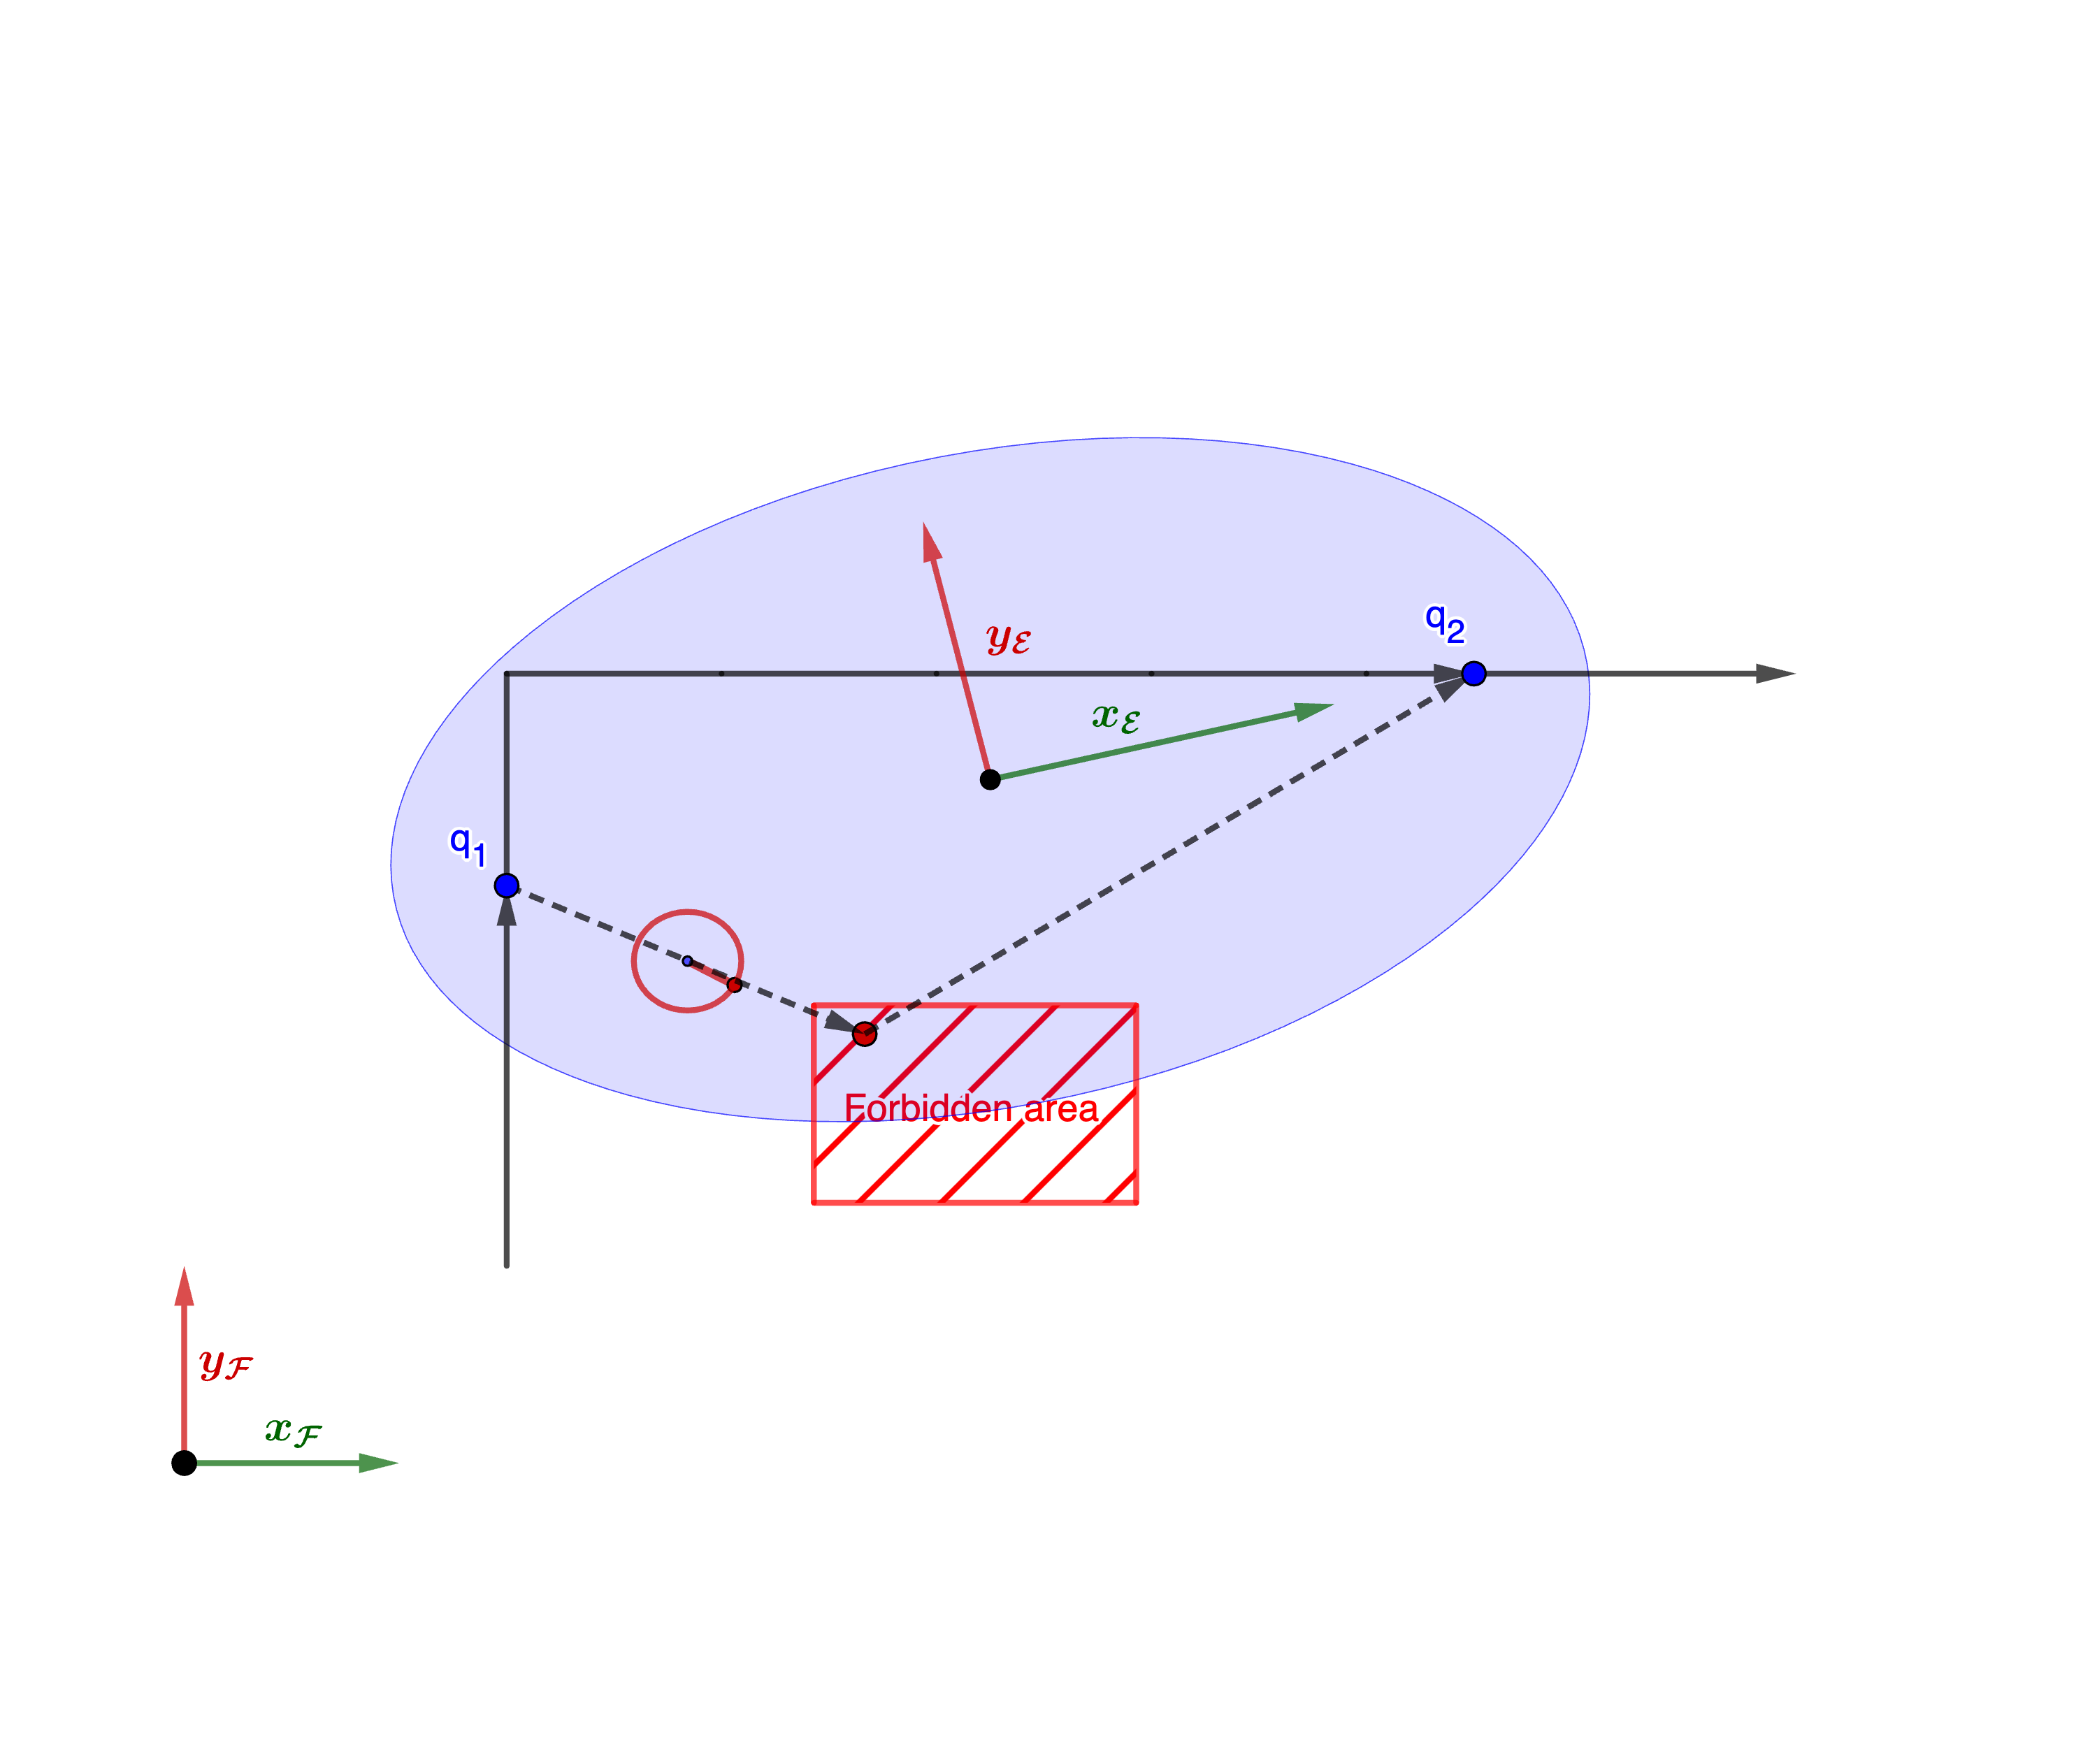
\includegraphics[width=0.8\linewidth, trim = 2cm 2.5cm 2cm 5cm]{Reachability}
    \caption{The ellipse showcases the reachability region. The black line is the planned trajectory of a robot, $q_1$ and $q_2$ are two locations this robot are expected at given time $t_1$ and $t_2$, dashed line is a possible trajectory if the robot is compromised after reaching $q_1$. Axis of global frame $\cF$ and canonical frame $\cF_{\cE}$ are shown as $x_{\cF}, y_{\cF}$ and $x_{\cE}, y_{\cE}$ respectively. }
    \label{fig:EllipseConstraintExample}
  \end{figure}
 

The region $\cE(q_1,q_2)$ is an ellipsoid with foci at $q_1,q_2$, center $o_{\cE} = \frac{1}{2}(q_1+q_2)$, and the major radius equal to $a$. Let $c_\cE=\frac{1}{2}\norm{q_1-q_2}=\norm{o_\cE-q_1}$ be the distance from the center to a foci.

The reachability ellipsoid is an over-approximation of the exact reachability region; the difference between the two is due to the discretization of the trajectory, and the fact that $\cE$ does not consider the presence of obstacles.

\subsubsection{Transformation to canonical coordinates}\label{sec:rotation2Standard}
To simplify the problem, we employ a canonical rigid body transformation that repositions the ellipse $\cE$ from the global frame $\cF$ to a canonical frame $\cF_\cE$. 
The canonical frame $\cF_\cE$ is defined as the origin aligns with the ellipsoid's center, and the first axis aligns with the foci. We perform this transformation in a differentiable manner, with respect to the two foci serving as waypoints for a robot.
We parametrize the transformation from $\cF$ to $\cF_\cE$ using a rotation $R^\cF_\cE$ and a translation $o^\cF_\cE$, which, to simplify the notation, we refer to as $R$ and $o$, respectively. 
The transformation of a point from the frame $\cF_\cE$ to the frame $\cF$ and its inverse are given by the rigid body transformations:
  \begin{equation}\label{eq:transformations}
    \Fframe{q}=R\Eframe{q}+o,\quad
    \Eframe{q}=R\transpose(\Fframe{q}-o).
  \end{equation}
 
  We define $\nu_\cF$ and $\nu_\cE$ to represent the $x$-axis unitary vector of $\cF_\cE$ in the frames $\cF$ and $\cF_\cE$, respectively. Formally:
  \begin{align}
    \nu'_\cF&=q_2-q_1, & \nu_\cF &= \frac{\nu'_\cF}{\norm{\nu_\cF}}, & \nu_\cE&=[1,0,0]^T;
  \end{align}
  see Fig.\ref{fig:EllipseConstraintExample} for an illustration. Note that $\nu_\cE$ is constant while, for the sake of clarity, $\nu_{\cF}$ depends on $q_1,q_2$. From the definition of $\cF_\cE$, the rotation $R$ can be found using a \emph{Householder rotation}, while from \eqref{eq:transformations} the translation $o$ must be equal to the center of $\cE(q_1,q_2)$ expressed in $\cF$, i.e.:
  \begin{align} 
    R&=H(\nu_\cF(q_1,q_2),\nu_\cE(q_1,q_2)), &o&=\frac{1}{2}(q_1+q_2).
  \end{align}
  To simplify notation, in the following, we will consider $H$ to be a function of $q_1,q_2$ directly, i.e. $H(q_1,q_2)$. 
  The ellipse $\cE$ expressed in $\cF_\cE$ is given by $\Eframe{\cE}=\{\Eframe{q}\in\real{m}:d(q^\cE_1,\Eframe{q})+d(\Eframe{q},q^\cE_2)<2a\}$, where the coordinates of the two foci $q^\cE_1,q^\cE_2$ in $\cF_\cE$ are
  \begin{align}
    q^\cE_1=\bmat{c & 0 & 0}\transpose, && q^\cE_2=\bmat{-c & 0 & 0}\transpose,
  \end{align}
  with $c=\frac{\norm{q_2-q_1}}{2}$.
\begin{definition}
  The \emph{reachability ellipsoid $\cE$ in the canonical frame} is defined as as the zero level set of the quadratic function
  \begin{equation}\label{equ:standard-ellipse}
    \Eframe{E}(\Eframe{q}) = \Eframe{q}\transpose Q \Eframe{q} - 1
  \end{equation}
  where
  \begin{equation}
    Q = \diag(a^{-2},b^{-2},b^{-2}),
  \end{equation}
  and $b = \sqrt{a^2-c^2}$.
  The ellipse parameters $a$, $b$ represent the lengths of the major axes.
\end{definition}
\begin{lemma}
The original ellipse $\cE$ in $\cF$ can be expressed as the zero level set of the quadratic function
   \begin{equation}\label{eq:ellpsoid from canonical}
     \Fframe{E}(\Fframe{q}) = (\Fframe{q}-o_\cE)\transpose H\transpose Q H (\Fframe{q}-o_\cE) - 1
     \end{equation}
\end{lemma}
\begin{proof}
    The claim follows by substituting  \eqref{eq:transformations} into \eqref{equ:standard-ellipse}, and from the definition of $R$ and $o$.
\end{proof}
For all reachability ellipsoid constraints, we first solve the problem in the canonical frame $\cF_{\cE}$, and transform the solutions to the global frame $\cF$ using the transformation \eqref{eq:transformations}.

We are now ready to formulate constraints based on reachability ellipsoids against different types of forbidden regions: a point, a plane, a segment, and a convex polygon. For each one, our goal is to define the function $D(q)$, its differential $\partial_qD(q)$, the set $\zeta$ and the projection $\Pi_\zeta$ that can be incorporated in the ADMM optimization (\ref{eq:ADMMSetConstraint_modified}).

\subsection{Point-ellipsoid reachability constraint}\label{sec:ellipsoid-point}
\zyang{change this to a circle by adding radius to projection?}
As shown in Fig.\ref{fig:Ellipse-to-point}, we consider a forbidden region in the shape of a single point $q_{avoid}$. The goal is to design the trajectory $q(t)$ such that $q_{avoid}\notin\mathcal{E}(q_1,q_2)$. This constraint can be written as, 

\begin{constraint}[Point-ellipsoid reachability constraint]
\begin{align}
D(\vq) &=  \begin{cases}
      \pi_{p\cE}(q) - q_{avoid} & q_{avoid} \in \cE, \\
      {0} & \textrm{otherwise}.
    \end{cases} \label{eq:point_ellipsoid_constraint}\\
  \sZ &= \{q\in\mathbb{R}^{nm}:\norm{D_p(q)} = 0 \},\\
   \Pi_\sZ(z) & = 0, 
\end{align}
\end{constraint}

where $\pi_{p\cE}(q_{avoid};q_1,q_2,a) = q_p$ is a projection function that returns a projected point $q_p$ of $q_{avoid}$ outside the ellipse, i.e., as the solution to
\begin{equation}\label{eq:ellipse-point-projection}
\pi_{p\cE}=\argmin_{q_p\in\cE^c} \quad \norm{q_{avoid}-q_p}^2 
\end{equation}
where $\cE^{c}$ is the set complement of the region $\cE$.
  
\begin{figure}[htbp]
\begin{center}
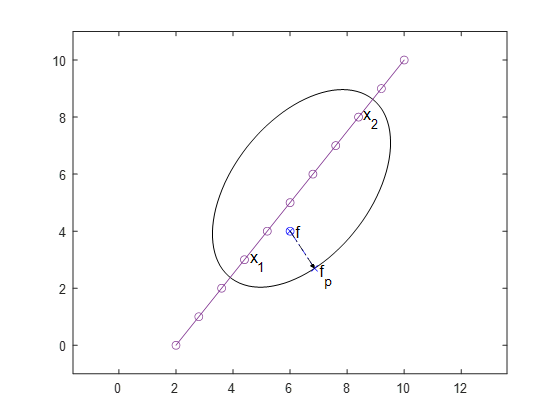
\includegraphics[width=0.6\linewidth, trim = 1.5cm 2.5cm 1.5cm 3cm, clip]{Ellipse2point}
\caption{Point-ellipsoid constraint, a point $q_{avoid}$ inside ellipsoid is projected to the areas outside the ellipsoid $f_{p}$.}
\label{fig:Ellipse-to-point}
\end{center}
\end{figure}

  For cases where $q_{avoid} \notin \cE(q(t_2),q(t_1),r)$, $\pi_{p\cE}(q_{avoid}) = q_{avoid}$. And for cases where $q_{avoid} \in \cE(q_1,q_2,r)$, $D(q)$ needs to be projected to the boundary of the ellipse. In canonical frame $\cF_{\cE}$, the projected point $q^{\cE}_{p}$ can be written as:
  \begin{equation}
  	q^\cE_{p} = {(I+sQ)}\inverse q^\cE_{avoid} = S q^\cE_{avoid}
  \end{equation}
  %where $S=(I+sQ)\inverse$.Using the fact that since $q^\cE_p$ is a point on the ellipse, 
  where $s$ can be solved as the root of the \eqref{equ:standard-ellipse}:
  \begin{equation}
    {q^\cE_p}\transpose Q q^\cE_p-1={q^\cE_{avoid}}\transpose Q'(s) q^\cE_{avoid} -1=0
  \end{equation}
  where
  \begin{equation}
    Q'(s) =S\transpose Q S = \diag\left(\frac{a^{2}}{(s+a^{2})^2}, \frac{b^{2}}{(s+b^{2})^2},\frac{b^{2}}{(s+b^{2})^2}\right)
  \end{equation}
 Detailed methods for computing $s$ can be found in \cite{yang2021multi} \cite{yang2020multi} \cite{eberly}. 


  %The point to project, $q_{avoid}$, can be likewise expressed in $\cF_\cE$ as $\Eframe{q}_{avoid} =  H (\Fframe q_{avoid}-o)$. We now turn our attention to the problem of projecting $\Eframe{q}_{avoid}$ on the zero level set of $E^\cE$ (i.e., the reachability ellipsoid in the canonical frame). The derivations below are loosely inspired by \cite{eberly}.

  %Let $q^\cE_p$ be the point on the surface of the ellipsoid, i.e., $\Eframe E(q^\cE_p) = 0$, corresponding to the projection of the point $q^\cE_{avoid}$. Using Lagrange multipliers applied to the constrained optimization problem \eqref{eq:ellipse-point-projection} (after transforming it in the canonical frame), one can show that the vector from a point to its projection, $q^\cE_{avoid}- q^\cE_p$, must be collinear with the gradient of $\Eframe \cE$, i.e.
 % \begin{equation}
 %   q^\cE_p- q^\cE_{avoid} = s \partial_q \Eframe E(q^\cE_p)\transpose = s Q q^\cE_p
  %\end{equation}
  %for some scale $s\in\real{}$;
 % thus $q^\cE_p$ can be written as:

  Then the point-to-ellipse projection function in $\cF$ can be represented as:
  \begin{multline}\label{equ:Point2EllipseProjection}
    \pi_{p\cE}(q)= R^{-1}(q(t_1),q(t_2))q^\cE_p+o \\
    = R^{-1}(q(t_1),q(t_2))Sq^\cE_{avoid}+o\\
    = R^{-1}S R ( q_{avoid}- o)+o
  \end{multline}
  
  In our derivations, we consider only the 3-D case ($m=3$); for the 2-D case, let $P=\bmat{I & 0}\in\real{2\times 3}$: then $\pi_{p\cE}^{\textrm{2D}}=P\pi_{p\cE}^{\textrm{3D}}(P\transpose q_{avoid}; P\transpose q_1, P\transpose q_2,a)$.

  \begin{proposition}\label{prop:Ellipse2PointDiff}
    The differential of the projection operator $\pi_{p\cE}(q_{avoid}; q_1,q_2,a)$ with respect to the foci $q_1,q_2$ is given by the following (where we use $q$ as a shorthand notation for $q^\cE_{avoid}$)
    \begin{multline}
      \partial_{\left[\begin{smallmatrix}q_1\\q_2\end{smallmatrix}\right]} \pi_{p\cE}=-2 H [ SH(q-o)]_{\times}U   \\
      + \left( (q\transpose \partial_sQ' q)^{-1} H^{-1} Q' q q\transpose  (4Q' H[q - o]_\times U \right. \\
      \left.+ 2Q' H\partial_q o - \partial_b Q' q q \partial_q b) -  s H^{-1} S^2 \partial_b Q q \partial_q b\right) \\
      -2H^{-1} S H[q-o]_{\times} U  + (H^{-1}SH -I)\partial_q o
    \end{multline}
  \end{proposition}
  \begin{proof}
  See \Cref{proof:Ellipse2PointDiff}.
  \end{proof}
  The differential of $D_p$ is the same as the one for $\pi_{p\cE}$.

\subsection{Plane-ellipsoid reachability constraint}\label{sec:ellipsoide-plane}

\begin{figure}[htbp]
\begin{center}
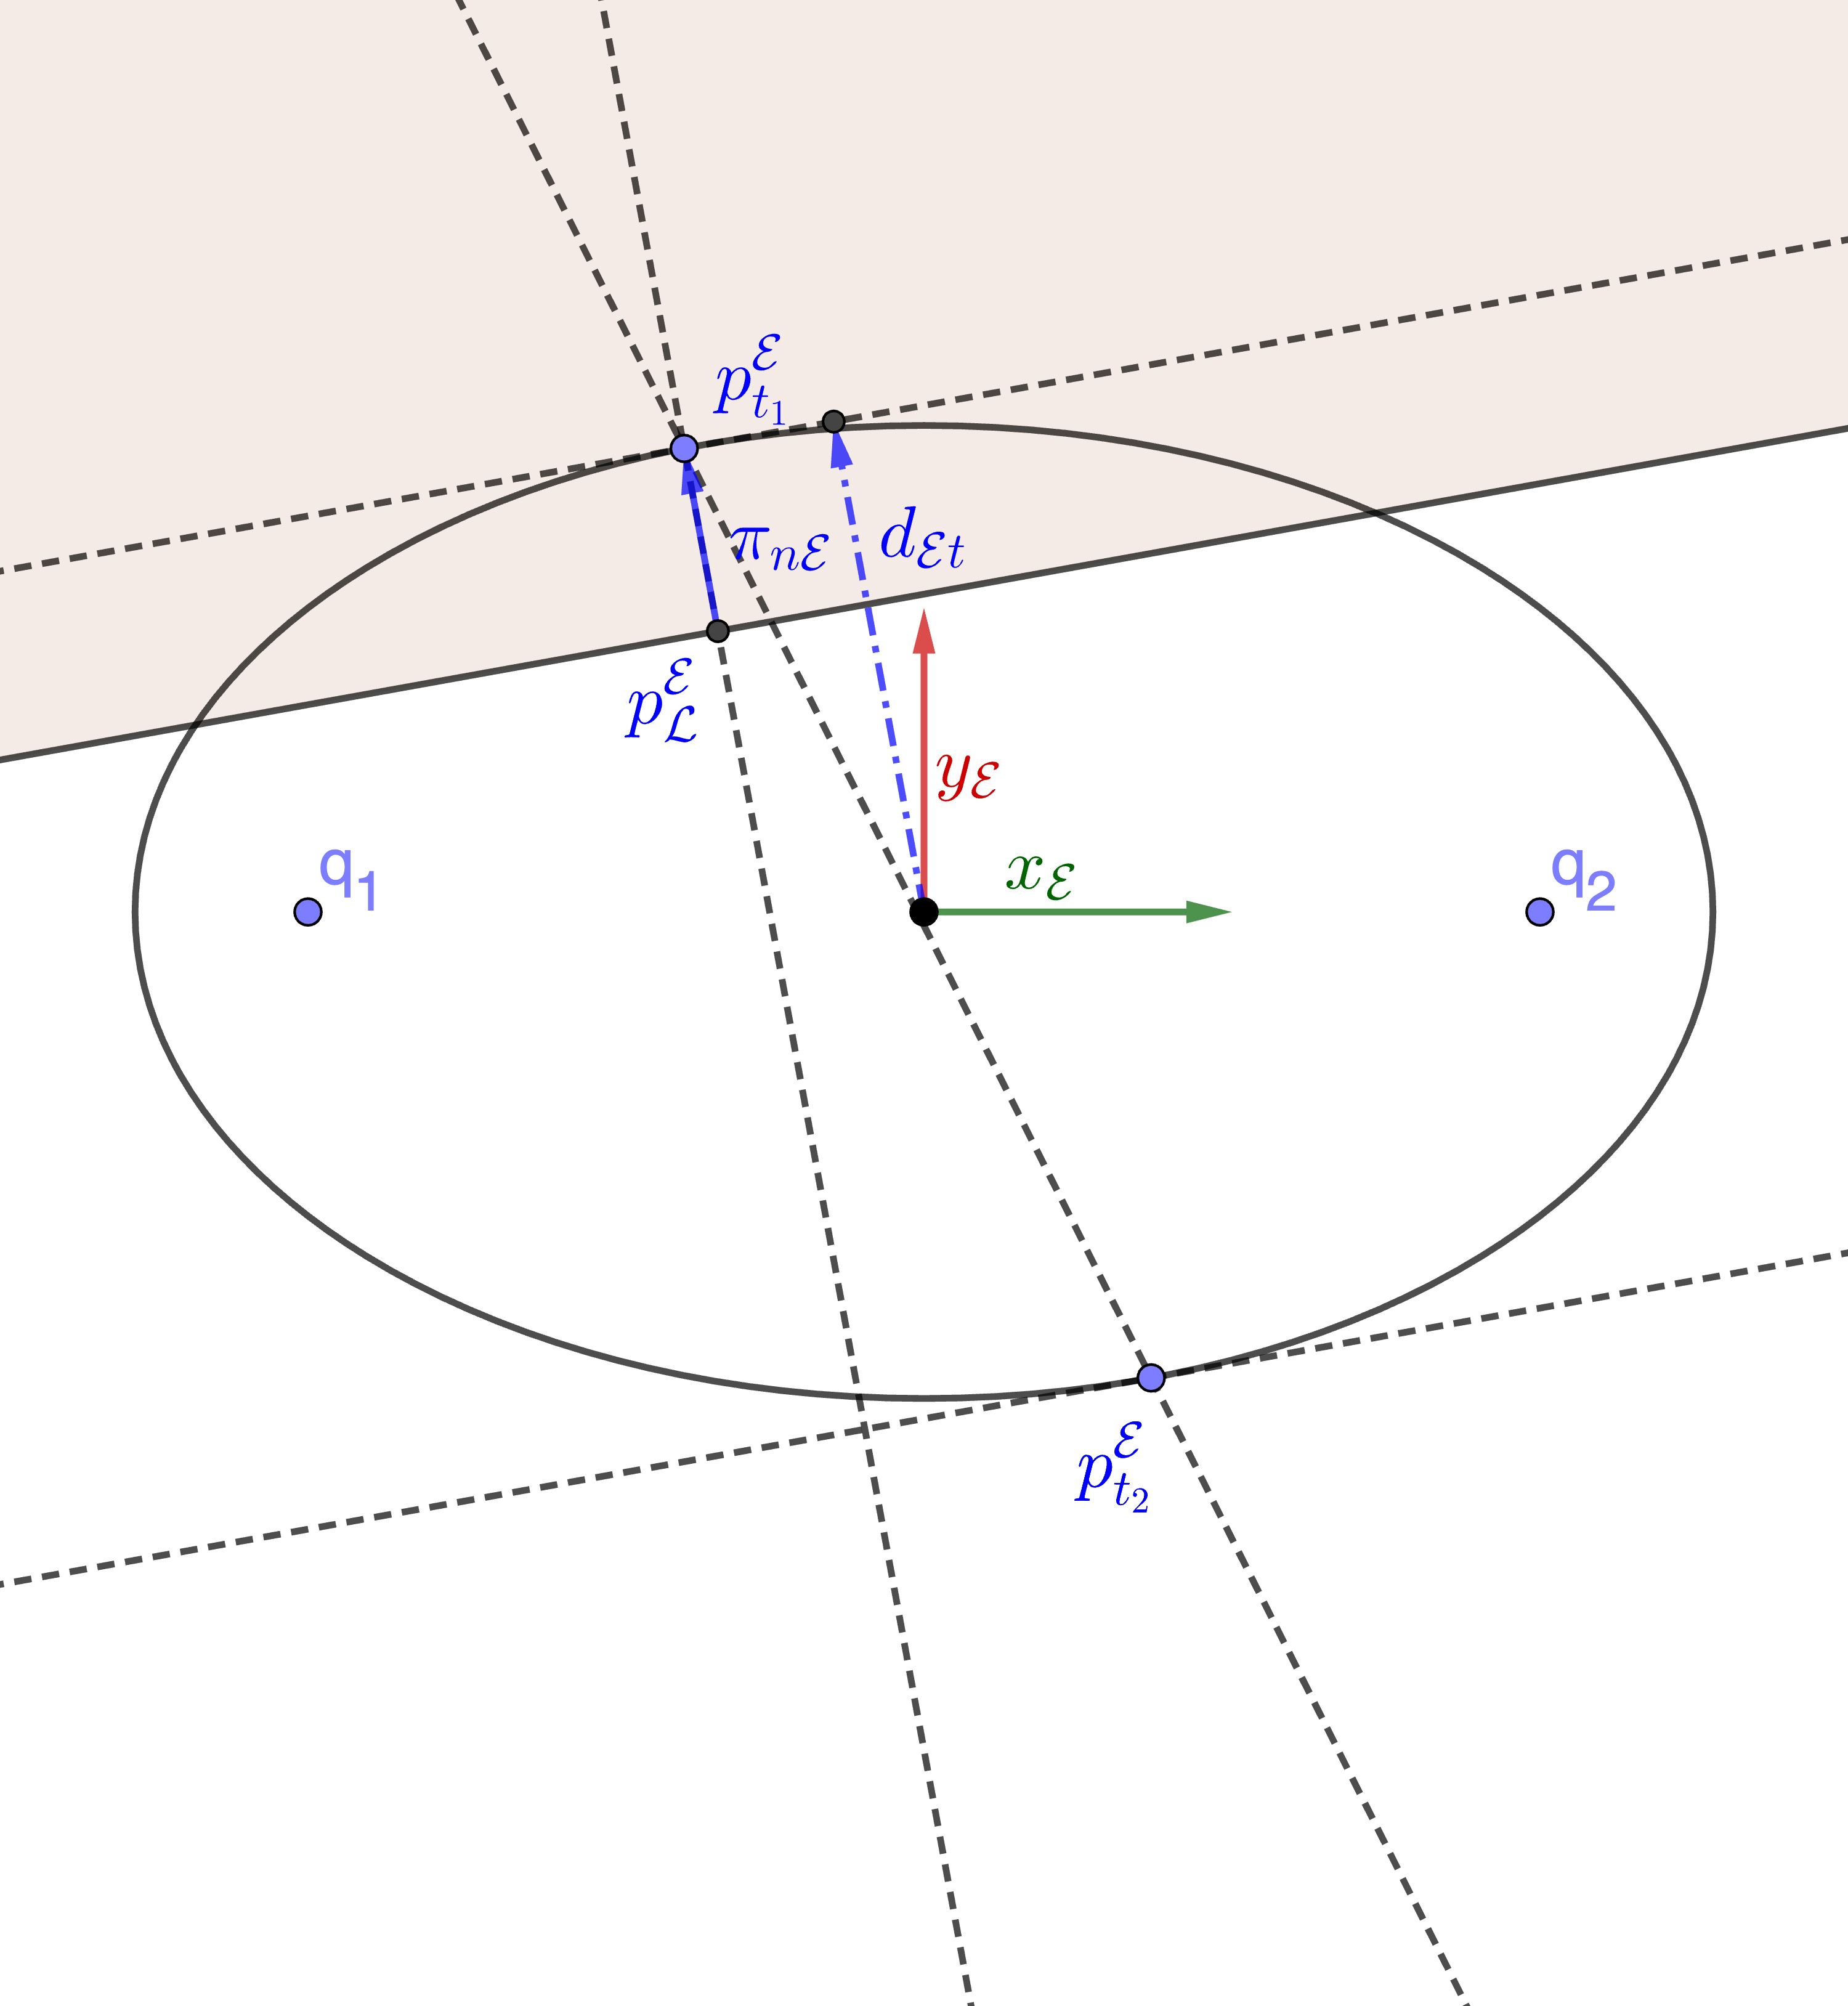
\includegraphics[width=0.6\linewidth, trim = 0cm 1.5cm 0cm 1cm, clip]{Ellipse2line_V2}
\rtron{Add $d_{\cE t}$}
\caption{Plane-ellipse constraint. Projected a ellipsoid to one side of a plane. The projection is simplified to the point-ellipse constraint as projecting a point inside ellipse $p_{L}$ to $p_{t}$ on outside the ellipse.}
\label{fig:Ellipse-to-plane}
\end{center}
\end{figure}

For forbidden region in the shape of a hyperplane $\mathcal{L}(\tilde{q}) = \{\tilde{q}\in\mathbb{R}^n: \vn\transpose \tilde{q} = d\}$ (as shown in Figure \ref{fig:Ellipse-to-plane}). The reachability constraint now can then be defined as $\mathcal{L} \cap \mathcal{E}(q_1,q_2,a) = \emptyset$. When transformed into canonical frame, the hyperplane can be written as $\Eframe \cL(\tilde{q}) = \{  \tilde{q}\in\mathbb{R}^m:  \vn_\cE\transpose \tilde{q} = d_{\cE}\}$, where,
  \begin{equation}
    n_\cE = H(q_1,q_2)n, \quad d_\cE =-\vn\transpose o + d.
\end{equation}
Intuitively, $d_\cE$ can be thought as a distance between the the plane $\cL$ and the origin (i.e., the center of $\cE$).
For every $\Eframe \cL(\tilde{q})$, there always exist two planes that are parallel to $\cL$ and tangent to the ellipse, $\cL_1^{\cE} = \{\tilde{q}\in\mathbb{R}^m: \vn_\cE \transpose \tilde{q} =  d_{\cE t} \}$ and $\cL_2^{\cE} = \{\tilde{q}\in\mathbb{R}^m: \vn_\cE \transpose \tilde{q} = - d_{\cE t} \}$  (\Cref{fig:Ellipse-to-plane}).
\rtron{Move the definition of tangents, tangent points, and tangent interpolation point here}

With these definitions, the constraint can be written as:

\begin{constraint}[Plane-ellipsoid reachability constraint]
\begin{align}
D(\vq) &= H^{-1}(q(t_1),q(t_2))\pi^\cE_{\vn_\cE}(q)+o, \label{eq:plane_ellipsoid_constraint}\\
  \sZ &= \{q\in\mathbb{R}^{nm}:\norm{D_{\vn}(q)} = 0 \},\\
   \Pi_\sZ(z) & = \overrightarrow{0}, 
\end{align}
\end{constraint}
\rtron{Check that $q$ is $\vq$ where necessary. Also sometimes you use $q(t_1),q(t_2)$ and sometimes $q_1,q_2$, check for consistency.}
where $\pi^\cE_{\vn_\cE}(q)$ is the projection operator defined as:
  \begin{equation}\label{equ:plane2ellipse}
    \pi^\cE_{\vn_\cE}(q) =\begin{cases}
      p^\cE_{1}-p^\cE_{\cL} & \textrm{ if } d_\cE \in [0, d_{\cE t}], \\
      p^\cE_{2}-p^\cE_{\cL} &  \textrm{ if } d_\cE \in [- d_{\cE t},0), \\
      {0} & \textrm{otherwise}.
    \end{cases}
  \end{equation}
$p^\cE_1$ and $p^\cE_2$ are tangent points on two planes that are parallel to $\cL$ and tangent to the ellipse, $\cL_1^{\cE} = \{\tilde{q}\in\mathbb{R}^m: \vn_\cE \transpose \tilde{q} =  d_{\cE t} \}$ and $\cL_2^{\cE} = \{\tilde{q}\in\mathbb{R}^m: \vn_\cE \transpose \tilde{q} = - d_{\cE t} \}$  (\Cref{fig:Ellipse-to-plane}). Analytically, these points can be found as 
 \begin{equation}
    p^\cE_{1} = \frac{ d_{\cE t} Q^{-1}   n_\cE}{ n_\cE \transpose Q^{-1}  n_\cE} = \frac{Q^{-1} n_\cE}{ d_{\cE t}},\quad  p^\cE_{2} = -  p^\cE_{1},
  \end{equation}
where $d_{\cE t} = \sqrt{ n_\cE\transpose Q^{-1} n_\cE}$; intuitively, $d_{\cE t}$ can be thought as a distance between the tangent planes $\cL_1^\cE$, $\cL_2^\cE$ and the origin (i.e., the center of the ellipse $\cE$).
The \emph{tangent interpolation point} $p^\cE_{\cL} \in \mathcal{L}$ is defined on the plane by 
    \begin{equation}\label{equ:ProjectPoint}
      p^\cE_{\cL} = \frac{ d_\cE Q^{-1} n_\cE}{ n_\cE\transpose Q^{-1} n_\cE}.
    \end{equation}
  Intuitively, the point $p^\cE_\cL$ is the point on $\cL$ which is closest to either $p^\cE_1$ or $p^\cE_2$.
  Note that when  $d_\cE=d_{\cE t}$ or $d_\cE=-d_{\cE t}$, $p^\cE_{\cL}=p^\cE_{1}$ or $p^\cE_{\cL}=p^\cE_{2}$, respectively. When $ d_\cE \in [- d_{\cE t},  d_{\cE t}]$, the plane $\cL$ and the ellipsoid $\cE$ have at least one intersection, thus violating our desired reachability constraint. 

  \begin{proposition}\label{prop:dpi_ne_dt}
    The differential of the projection function $\pi^\cE_{\vn \cE}(q)$ with respect to the foci $q_1$ and $q_2$ is given by:
    \begin{equation}
      \partial_q \pi^\cE_{\vn \cE}(q) = \begin{cases}
        \partial_q p^\cE_{t1}-\partial_q p^\cE_{\cL} &  d_\cE \in [0, d_{\cE t}], \\
        \partial_q p^\cE_{t2}-\partial_q p^\cE_{\cL} &  d \in [- d_{\cE t},0), \\
        {0} & otherwise.
      \end{cases}
    \end{equation}
    where
    \begin{multline}
      \partial_q p_\cL =   (-\frac{d_{\cE t} n\transpose \partial_q o -2d_\cE \partial_q d_{\cE t}}{d_{\cE t}^3} )Q^{-1}n_\cE \\
      + \frac{d_\cE\partial_b Q^{-1} n_\cE \partial_q b -  2d_\cE Q^{-1}H[n]_\times U}{d_{\cE t}^2},
    \end{multline}
    \begin{equation}
      \partial_q p_{1} =  -\frac{Q^{-1}n_\cE \partial_q d_{\cE t} }{d_{\cE t}^2} 
      + \frac{\partial_b Q^{-1}n_\cE \partial_q b -  2Q^{-1}H[n]_\times U }{d_{\cE t}}.
    \end{equation}
  \end{proposition}
  \begin{proof}
  See \Cref{proof:dpi_ne_dt}.
  \end{proof}
  Based on the previous proposition, the differential of (\ref{eq:plane_ellipsoid_constraint}) can be written as:
  \begin{equation}
    \partial_q {D_{\vn\cE}} = -2 H \cross{\Eframe \Pi_{\vn \cE}}  M + H^{-1}\partial_q \Eframe \Pi_{\vn \cE}
  \end{equation}

\subsection{Line-segment-ellipse reachability constraint}\label{chapter:ellipse to segment}

\begin{figure}[htbp]
\begin{center}
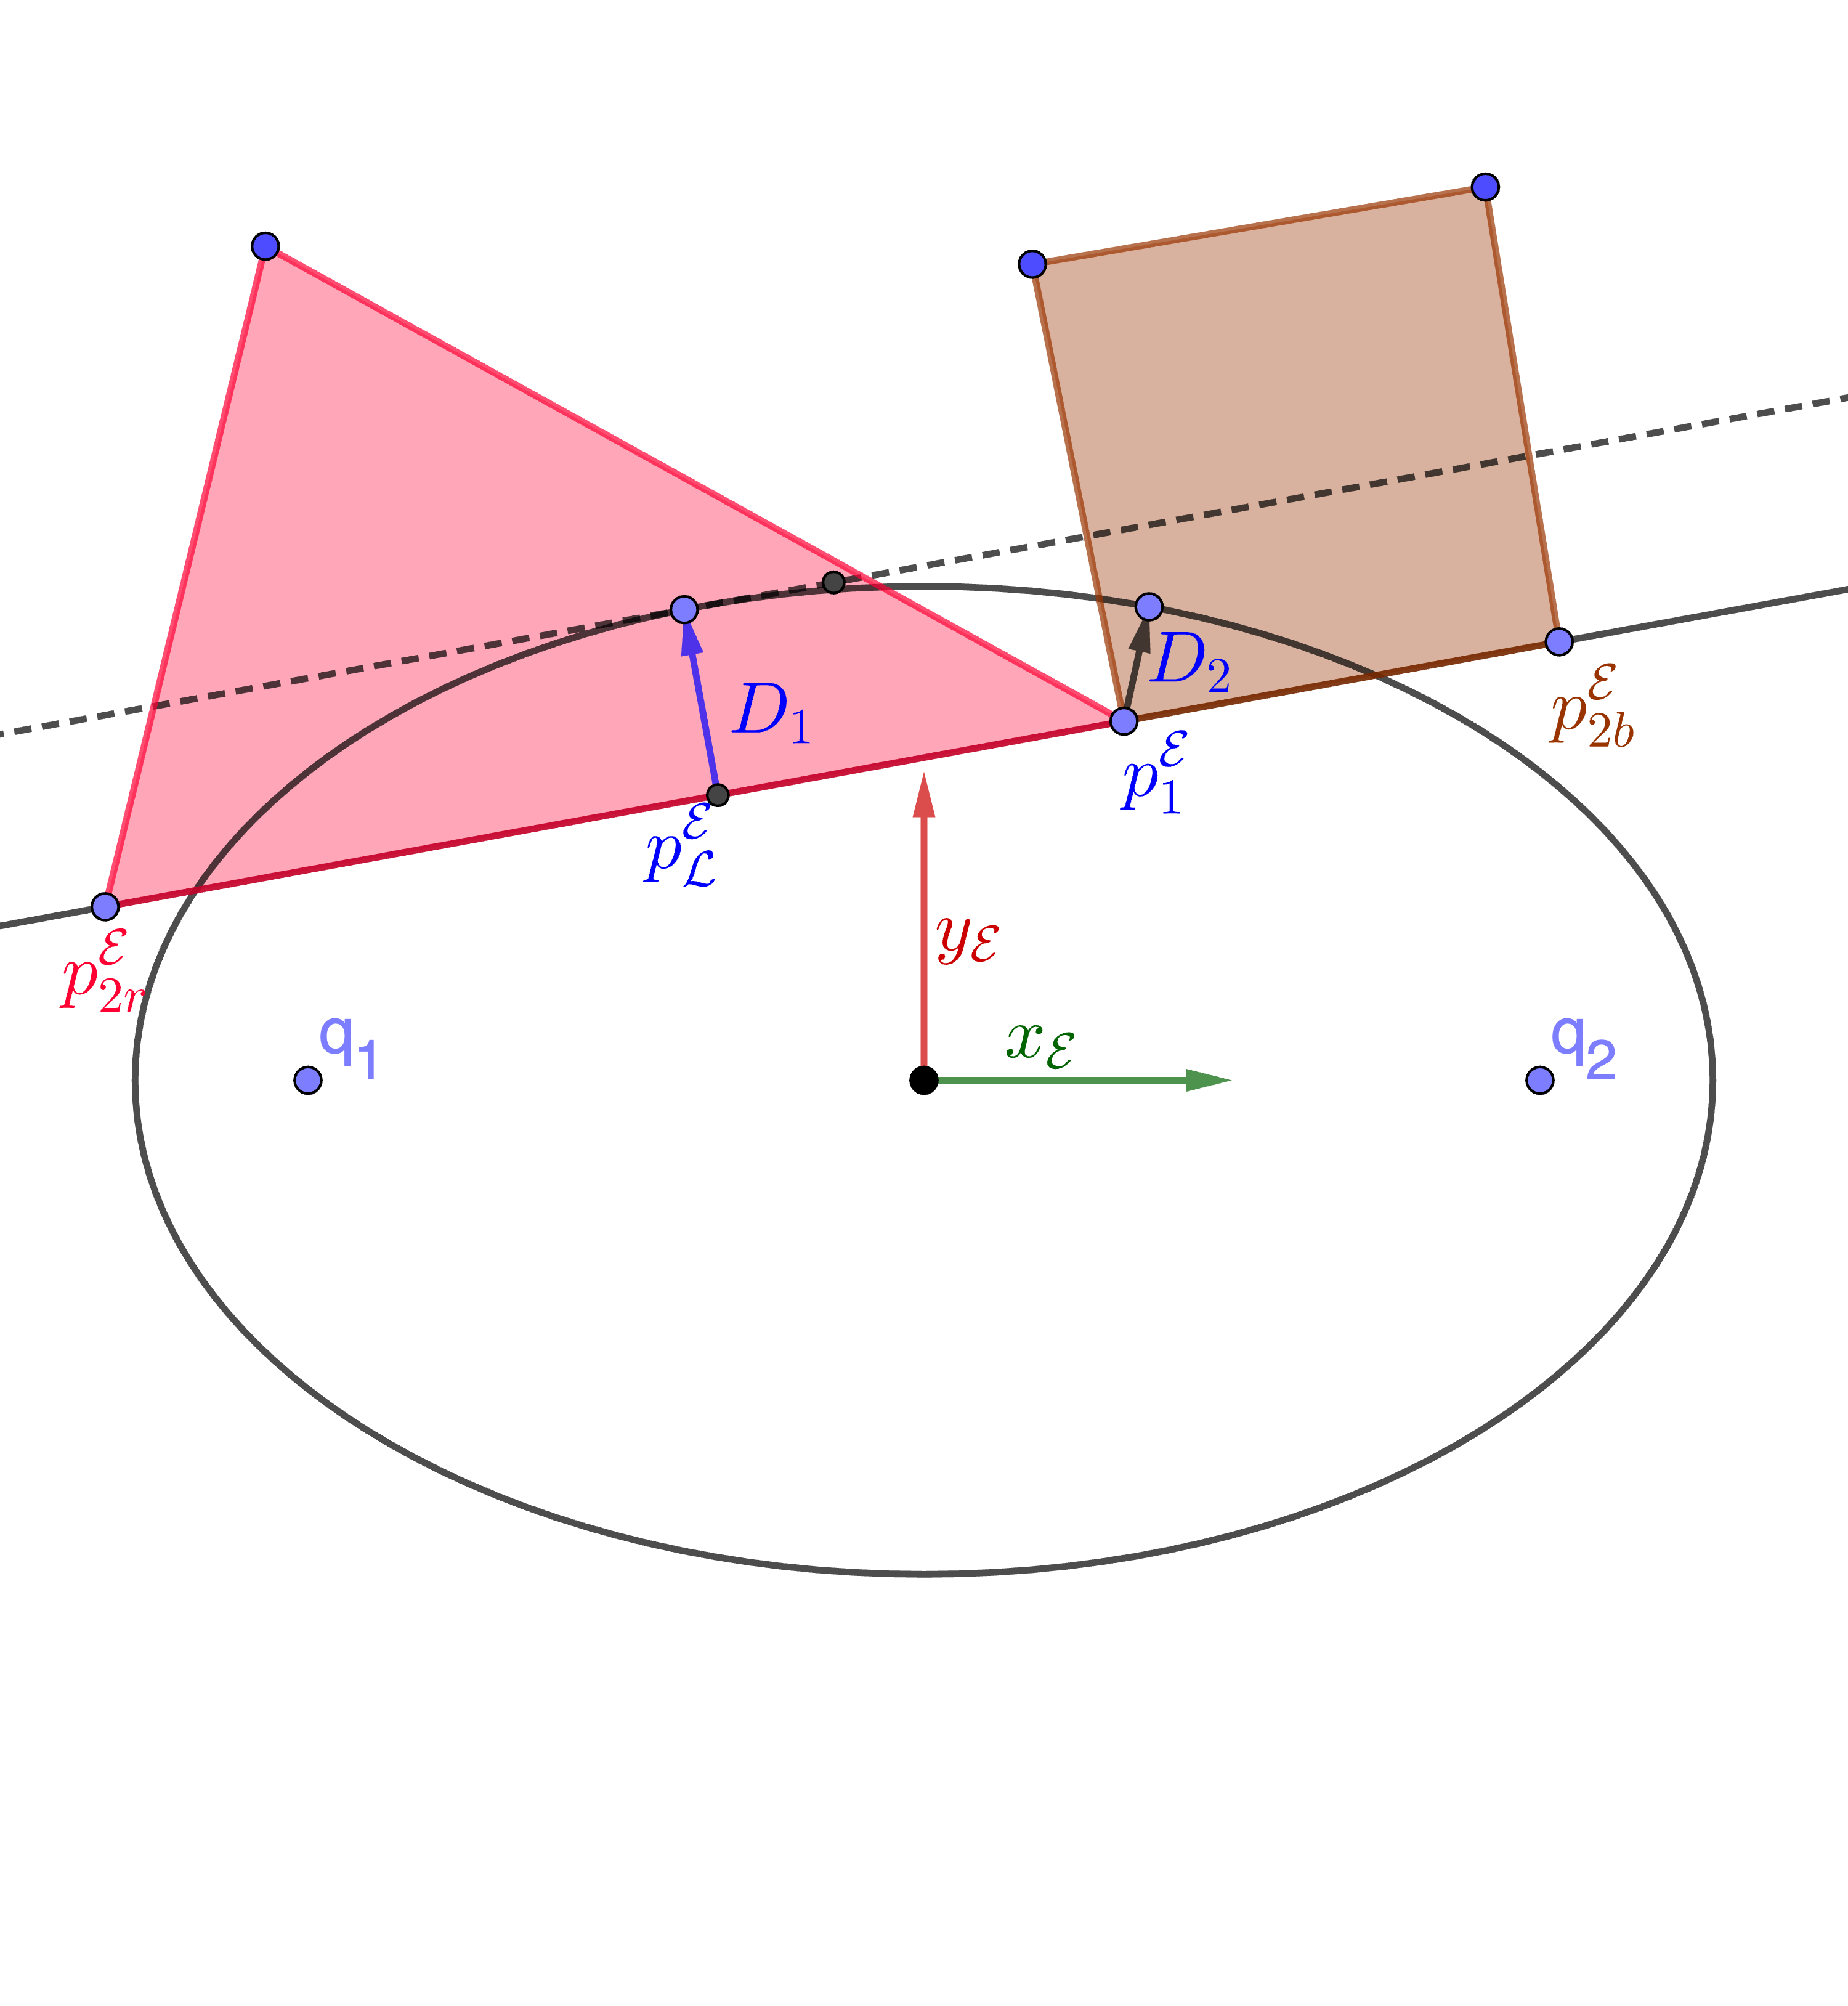
\includegraphics[width=0.6\linewidth]{Ellipse2safezone_V2}
\caption{Polygon-ellipse constraint. This constraint is simplified to either a plane-ellipse constraint or a point-ellipse constraint.}
\label{fig:Ellipse-to-safezone}
\end{center}
\end{figure}

For a intermediate step to get the relationship between a polygon shaped forbidden region, the relative position between the ellipse and segment of the hyperplane that defines the region is studied. 
Assume the segment has endpoints $p_1$ and $p_2$; then the segment can be defined as:
\begin{equation}
\bmat{(p_1-p_2)\transpose\\(p_2-p_1)\transpose} p \leq \bmat{p_2\transpose\\-p_1\transpose}(p_1-p_2)
\end{equation}
\rtron{Needs an additiona constraint that $p$ needs to be on the line $p_1p_2$.}
\begin{constraint}[Line-segment-ellipsoid reachability constraint]
\begin{align}
D(\vq) &=  \begin{cases}
D_1(p_1) & (p_1-p_2)\transpose (p_{\cL}-p_2)<0\\
D_1(p_2) & (p_2-p_1)\transpose (p_{\cL}-p_1)<0\\
D_2(p_{\cL}) & \textrm{otherwise}
\end{cases} \label{eq:segment_ellipsoid_constraint}\\
  \sZ &= \{q\in\mathbb{R}^{nm}:\norm{D_p(q)} = 0 \},\\
   \Pi_\sZ(z) & = 0, 
\end{align}
\end{constraint}

\rtron{Define $D_1$, $D_2$. Give intuition about what they represent.}
\subsection{Convex-polygon-ellipse reachability constraint}\label{sec:ellipse-region-constraint} 
To keep an ellipse away from a convex polygon, first, we need to keep all segments of the hyperplanes outside the ellipse. Similar to \eqref{equ:ProjectPoint}, we define
\begin{constraint}[Convex-polygon-ellipsoid reachability constraint]\label{constraint:polygon-ellipsoid}
\begin{align}
D(\vq) &= \bmat{D_{seg1}\\D_{seg2}\\ \vdots} \label{eq:region_ellipsoid_constraint}\\
  \sZ &= \{q\in\mathbb{R}^{nm}:\norm{D_p(q)} = 0 \},\\
   \Pi_\sZ(z) & = 0, 
\end{align}
\end{constraint}
\rtron{$D_{seg1}, D_{seg2}$ need to be defined.}
ADMM constraint~\ref{constraint:polygon-ellipsoid} needs to be supplemented with a convex obstacle constraint for the polygon (as introduced in section \ref{sec:obstacle}) to prevent cases where the ellipse is a subset of the region.

\subsection{Secured planning results and limitation}
In this section, we apply our ADMM path planning algorithm to an instance of a map exploration problem (Figure~\ref{fig:ADMM-example-application}), and test the algorithm in both simulations and an experimental testbed. The environment to be explored, with three agents, is a $10m\times10m$ region and two forbidden regions \emph{Zone 2, 3} which is shown in Fig.\ref{fig:Grid-example-application}.We assume that the robots can meaningfully collect information on the underlying vector field for data locations no further than $3m$. The maximum velocity constraint $v_{max}$ is set to~$0.5m/dt$ a time limit of 20. 

We utilize the APMAPF solver introduced in \cite{wardega2019resilience} to generate a MAPF plan with co-observation schedule on a grid-world application (Fig.\ref{fig:Grid-example-application}) and transform the result to a continuous configuration space, under the map exploration tasks.  All robots have the task of collecting sensor information on the underlying vector field, with agent 3 having an additional task to visit the \emph{checkpoint} at time $8$. Assuming that the sensors on the robots return data with higher accuracy for locations closer to the agent, the robots should ideally perform a boustrophedon pattern (like the unconstraint result in Figure~\ref{fig:trajectories-base}). We first set up an co-observation schedules considering two forbidden regions using the APMAPF algorithm, and add reachability constraints ensure a empty intersection between all robots' reachability regions between co-observations and forbidden regions.

As shown in Fig.\ref{fig:Grid-example-application}, no task has been assigned to the agent besides the start and goal location. Agent 1 and 2 need to meet at time 8 and 14, whereas agent 2 and 3 need to meet at time 18. This result is also used as the initial trajectory input for the ADMM solver. 

Based on the schedule, reachability for agent 1 in-between the scheduled co-observations are constrained. Notice that additional checkpoint (i.e. stationary security camera) need to be incorporated in order to generated an attack-proof solution. Additional solutions to avoid these checkpoints will be discussed in \Cref{chapter:cross-trajectory}.  

The result of the simulation is shown in Fig.~\ref{fig:ReachabilitySimulation}. The reachability regions are shown as black ellipsoids, and we can show that all of them have empty intersections with Zone 2 and 3. Notice that no explicit constraints have been enabled between reachability regions and obstacles, because we assume that robots have the basic obstacle avoidance capability and can not go through any hard obstacles. Therefore, the intersections between obstacles and ellipsoids, i.e. the case here between agent 3 and zone 1, are tolerable. All constraints have been satisfied and, to the best of their capability, agents have spread out across the map to perform the best possible exploration task. 

\begin{figure}[htbp]
\begin{center}
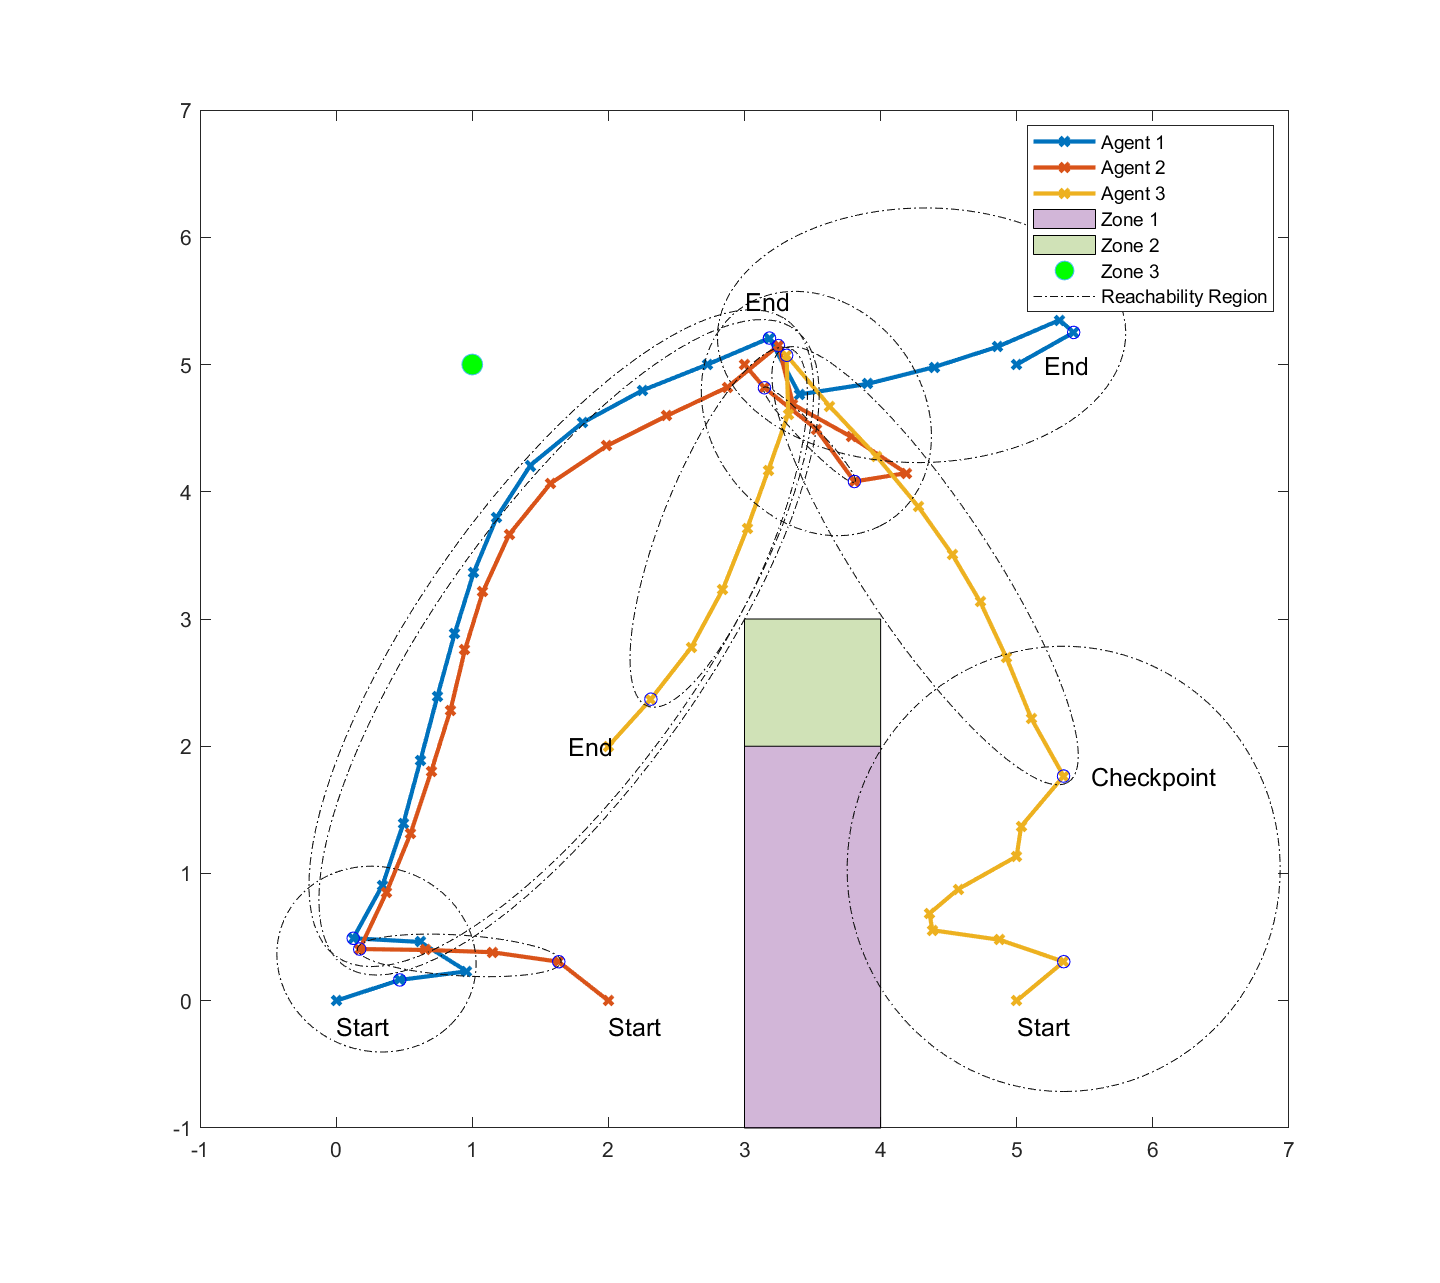
\includegraphics[width=0.6\linewidth]{FinalResult}
\caption{Simulation result for map exploration task. Reachability regions are shown as black ellipses in the result. Zone 1 is obstacle, Zone 2 and Zone 3 are safe zones}
\label{fig:ReachabilitySimulation}
\end{center}
\end{figure}

\subsubsection{Limitations}\label{sec:reachability-discussion}
Our solution shows that planning with reachability and co-observation is a promising approach to enhance the security of multi-agent systems. However, two main challenges have been identified in \cite{wardega2023hola}. Firstly, finding a co-observation and reachability secured plan may not always be feasible when robots are separated from others by obstacles or forbidden regions, or are located far away from each other. In such case, it is impossible for other robots to get close enough to establish co-observation schedules or find a reachability-secured path. Agent 3 in the Figure \ref{fig:ReachabilitySimulation} is a good example, as it required additional security checkpoint to create secured reachability areas. Secondly, security requirements may come at the cost of overall system performance, as illustrated by the comparison of Figure \ref{fig:trajectories-more-constraint} and \ref{fig:ReachabilitySimulation} where, after the introduction of security constraints, the top left corner is never explored by any robots. This is particularly concerning given that system performance is a key factor in the decision to use multi-agent systems. These challenges are addressed in Chapter \ref{chapter:cross-trajectory}, in order to ensure the effectiveness of planning with reachability and co-observation in securing multi-agent systems.

\section{Cross-trajectory co-observation planning}

To address the feasibility challenge and performance trade-off of the ADMM problem discussed in \Cref{sec:reachability-discussion}, we propose to form \emph{sub-teams} on each route, and setup additional co-observations both within the sub-team and across different sub-teams \rtron{refer to introductory figure}. 
These \emph{cross-trajectory co-observations} allow sub-teams to preserve the optimal unsecured trajectories (as shown in Figure \ref{fig:cross-traj-comparison-set}), as it does not require the entire \emph{sub-team} to maintain a close distance with other teams when co-observation occurs. 
Note that \emph{cross-trajectory co-observation}, are always preferred when feasible, since they provide better security in potential situations where the entire sub-team is compromised. \rtron{(More discussion in Sec. ??)}.

\rtronhl{Move to discussion}{In this section, we consider only the high-level path planning, while the assignment of the duties in the team will be performed dynamically, making it more difficult for attackers to successfully plan and execute attacks.}


\subsection{Problem overview}

\rtron{Introduce $n_p$ in the previous Section.}

In \Cref{sec:??} we assumed that the number of robot is equal to the number of routes $n_p$.
In this section, we  assume that we have a total of $n>n_p$ robots  available. \rtronhl{Clarify: since the robots change teams, this partition is time-varying, or can we get by without defining this partition explicitly?} We define a partition $\cI=\union_p \cI_p$ of the robots such that robots in \emph{sub-team} $\cI_p$ have the same nominal trajectory. We use the planner introduced in  \Cref{chapter:Multi-agent-ADMM} to generate multi-robot trajectories with $n_p$ routes $\{q_p\}_{p=1}^{N_p}$ without reachability and co-observation constraints, where the state $q_p(t), p \in\{0,\ldots,N_{p}\}$ represents the reference position of the $i$-th sub-team at time $t\in\{0, \dots, t_{e}\}$. \rtron{Again, make sure notation is consistent}
Within each sub-team, at least one robot is required to follow the reference trajectory to fulfill the required tasks. Meanwhile, the additional robots can switch from one reference trajectory to another in order to perform co-observation with different sub-teams. 
We refer to the new type of co-observations as \emph{cross-trajectory co-observations}. The goal is to find the cross trajectory co-observation plan to secure an unsecured MRS trajectory with a minimal number of additional robots.

\rtronhl{This can be summarized more, since it is discussed later in this same page}{To solve this problem, we model the planned trajectory $\{q_p\}_{p=1}^{N_p}$ as a directed \emph{checkpoint graph} $G_{q}=(V_{q}, E_{q})$. 
Vertices $V_{q}$ are a key locations in $\{q_p\}$ that are used to perform co-observations. Part of these vertices are \emph{checkpoints} which are selected to guarantee that, if robots deviate and reach forbidden regions, they will miss the scheduled co-observations. 
Other vertices are selected to connect checkpoints on different trajectories.
The set $E_{q} = E_{t} \union E_{c}$ consists of directed edges of two types, trajectory edges $E_{t}$ and cross-trajectory edges $E_{c}$, representing paths which robots can take. The trajectory edges $E_{t}$ represent the reference trajectories, where each edge connects two waypoints on the trajectory of the same sub-team. The cross-trajectory edges $E_{c}$ connect vertices on different reference trajectories, with at least one of the vertices being a checkpoint. These edges represent the potential paths that robots can take to travel and perform co-observations between trajectories of different sub-teams.} Similar to the work done by \cite{yu2013multi}, we show that additional robots in the sub-team can be formulated as flows in the checkpoint graph, transforming the co-observation planning problem into a network multi-flow problem that can be solved using general linear programming techniques as specialized solver. 

This section presents the two components of our approach: constructing the checkpoint graph based on unsecured multi-robot trajectories, and the formulation and solution of the network flow problem.

\subsection{Rapidly-exploring Random Trees}
In this section, we use the \rrtstar{} \cite{karaman2010incremental} algorithm to find paths from a single starting location to multiple destination points (i.e., the reference trajectories of other robots, in our method). \rtronhl{Move to the end of this RRT* section} Our objective is not to optimize specific constraints but to ascertain the existence of feasible paths. While the ADMM based solver \Cref{chapter:ADMM review} presented earlier offers a broader range of constraint handling, the RRT* algorithm is better suited to the problem in this section. RRT*'s efficient exploration of the solution space, coupled with its ability to incorporate obstacle constraints, makes it a fitting choice for building the checkpoint graph.

As a optimal path planning algorithm, \rrtstar{} returns the shortest paths between an initial location and points in the free configuration space, organized as a tree. We assume that the generated paths can be travelled in both directions (this is used later in our analysis). 
Key functions from \rrtstar{} that are also used during constructions of the checkpoint graph are
\begin{description}
\item[$\texttt{Cost}(v)$] This function assigns a non-negative cost (total travel distance in our application) to the unique path from the initial position to $v$ . 
\item[$\texttt{Parent}(v)$] This is a function that maps the vertex $v$ to $v'\in V$ such that $(v',v)\in E$.
\end{description}

\subsection{Checkpoint graph construction}

In this section, we describe in detail how we define and search for security checkpoints and how to use \rrtstar{} to construct the checkpoint graph $G_{q}$.

\subsubsection{Checkpoints}\label{sec:security-checkpoint}
Let $q\in\real{nmT}$ be the MRS trajectory found in Chapter \ref{chapter:Multi-agent-ADMM} for $m$ sub-teams with time horizon $T=t_{e}$, with $q_{p}(t)$ be the reference trajectory waypoint for sub-team $p$ at time $t$. A checkpoint $v_i=(q_{i},t_{i})$ is a pair composed of a location $q_{i}=q_{p}(t_{i})$ and a time $t_{i}$ representing a co-observation between a sub-team $\cI_p$'s member and robots either from the same sub-team or different ones. For convenience, let $\cI_{v_{i}}$ represent the sub-team $v_{i}$ belongs to. 

Similar to the requirements of co-observations introduced in  \Cref{chapter:Reachability_Constraints}, \rtronhl{Consider wrapping this in definition environment} {we define checkpoints $V_{p}=\{ v_{p_{1}}, \dots ,v_{p_{e}}\} \subset V_{q}$ for a reference trajectory $\{q_{p}(t)\}$ of sub-team $p$ in a way that guarantees that the reachability region between consecutive checkpoints $\mathcal{E}(q_{p_{i}}, q_{p_{i+1}}, t_{p_{i}},t_{p_{i+1}})$ does not intersect with any of the forbidden areas.}  The requirement can be formally stated as $\mathcal{E}(q_{p_{i}}, q_{p_{i+1}}, t_{p_{i}},t_{p_{i+1}}) \intersect F = \emptyset$ for every $i$, where $F$ is the union of all forbidden areas as $F$. 

We provide a heuristic approach to locate the checkpoints on given trajectories (an optimal solution would likely be NP-hard, while the approach below works well enough for our purpose). 
\rtron{State this as an Algorithm?} We begin by adding the start and end locations $q_{p}(t_{0})$, $q_{p}(t_{e})$ to $V_{q}$, where $t_{0}=0$, and $t_{e}$ is the time horizon. Then, we search for the waypoint $q_{p}(t_{1})$ with the largest $t_{1} \in \{t_{0}, \dots ,t_{2}\}$ such that the reachability ellipsoid between $q_{p}(t_{0})$ and $q_{p}(t_{1})$ has no overlap with any of the forbidden areas, i.e. $\mathcal{E}(q_{p}(t_{0}),q_{p}(t_{1}), t_{0},t_{1})\intersect F = \emptyset$. Simultaneously, we search backward to find $q_{p}(t_{3})$ with the smallest $t_{3}\in \{t_{1}, \dots ,t_{2}\} $ that meets the reachability requirement $\mathcal{E}(q_{p}(t_{2}),q_{p}(t_{3}),t_{2},t_{3}) \intersect F = \emptyset$. $q_{p}(t_{1})$ and $q_{p}(t_{3})$ are then added to $V_{q}$. Afterwards, we set $t_{0}=t_{1}$, $t_{2}=t_{3}$ and repeat the same process. The search is stopped when $t_{0}>t_{2}$, or when $\mathcal{E}(q_{p}(t_{0}),q_{p}(t_{2}),t_{0},t_{2}) \intersect F = \emptyset$. A toy example is shown in Figure \ref{fig:checkpoint-generate}. 

\begin{figure}
	\centering
    \subfloat[]{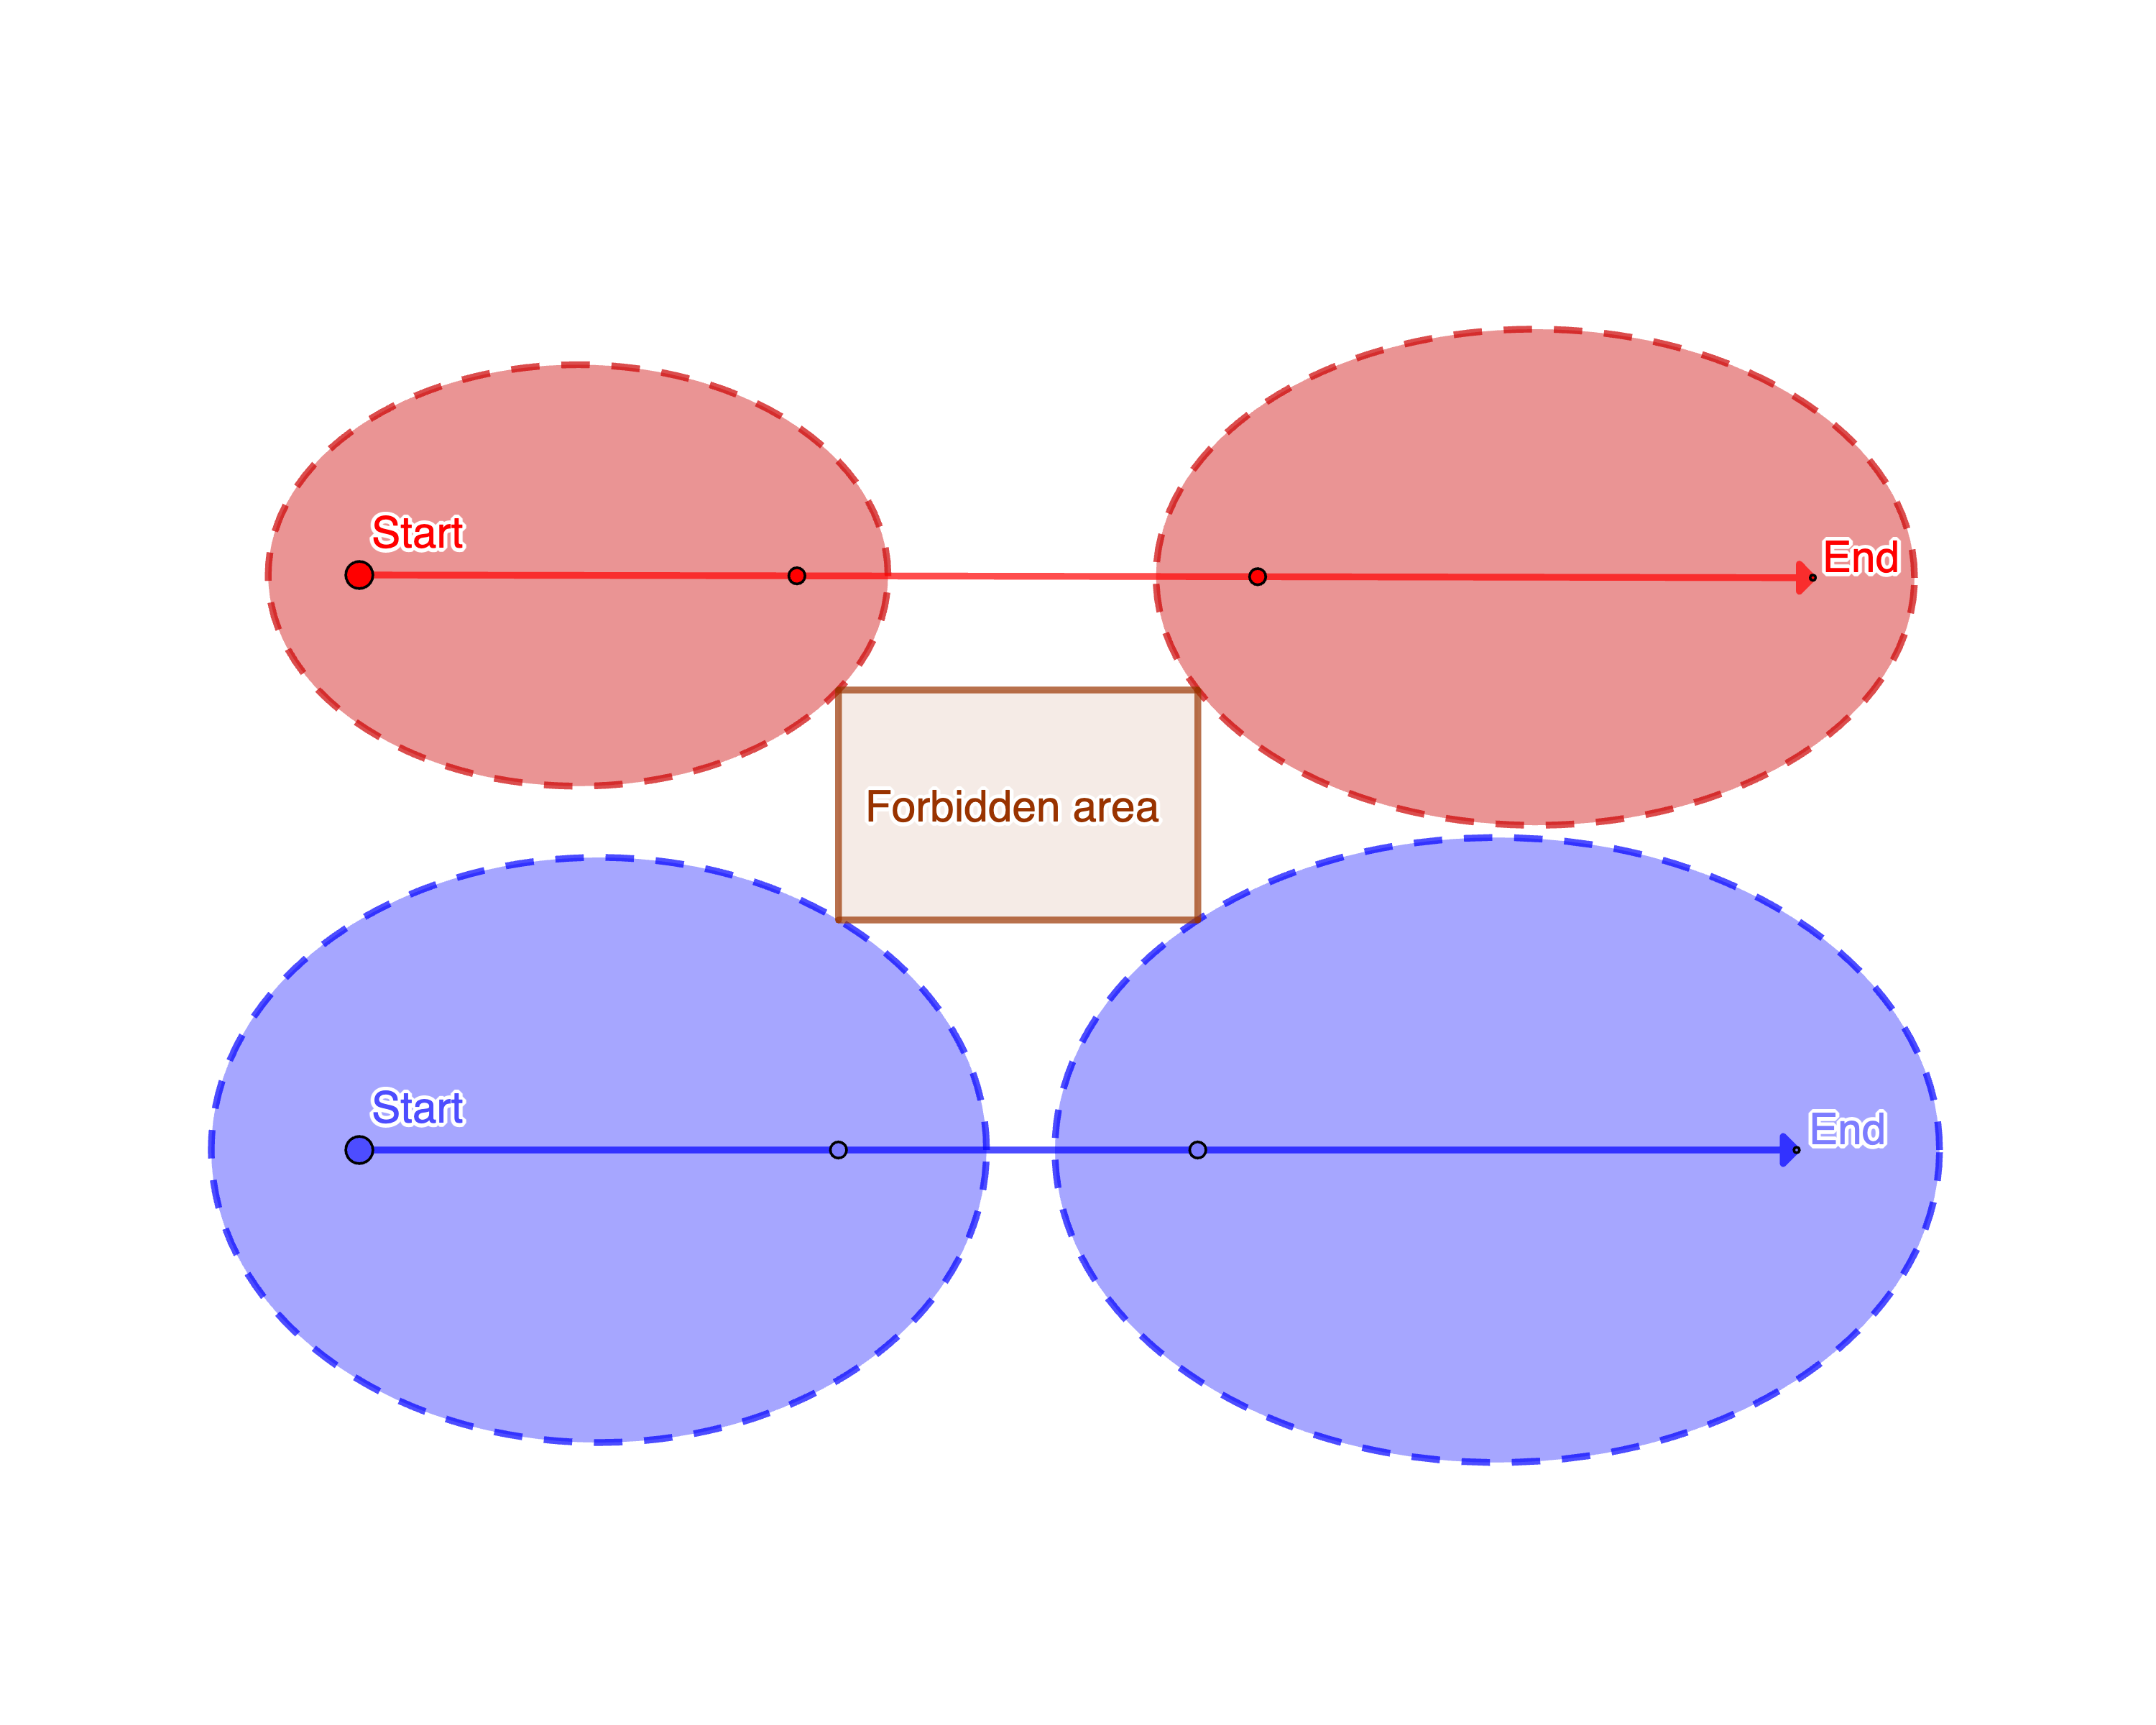
\includegraphics[width=0.45\linewidth]{SC_gen_1}}
    \subfloat[]{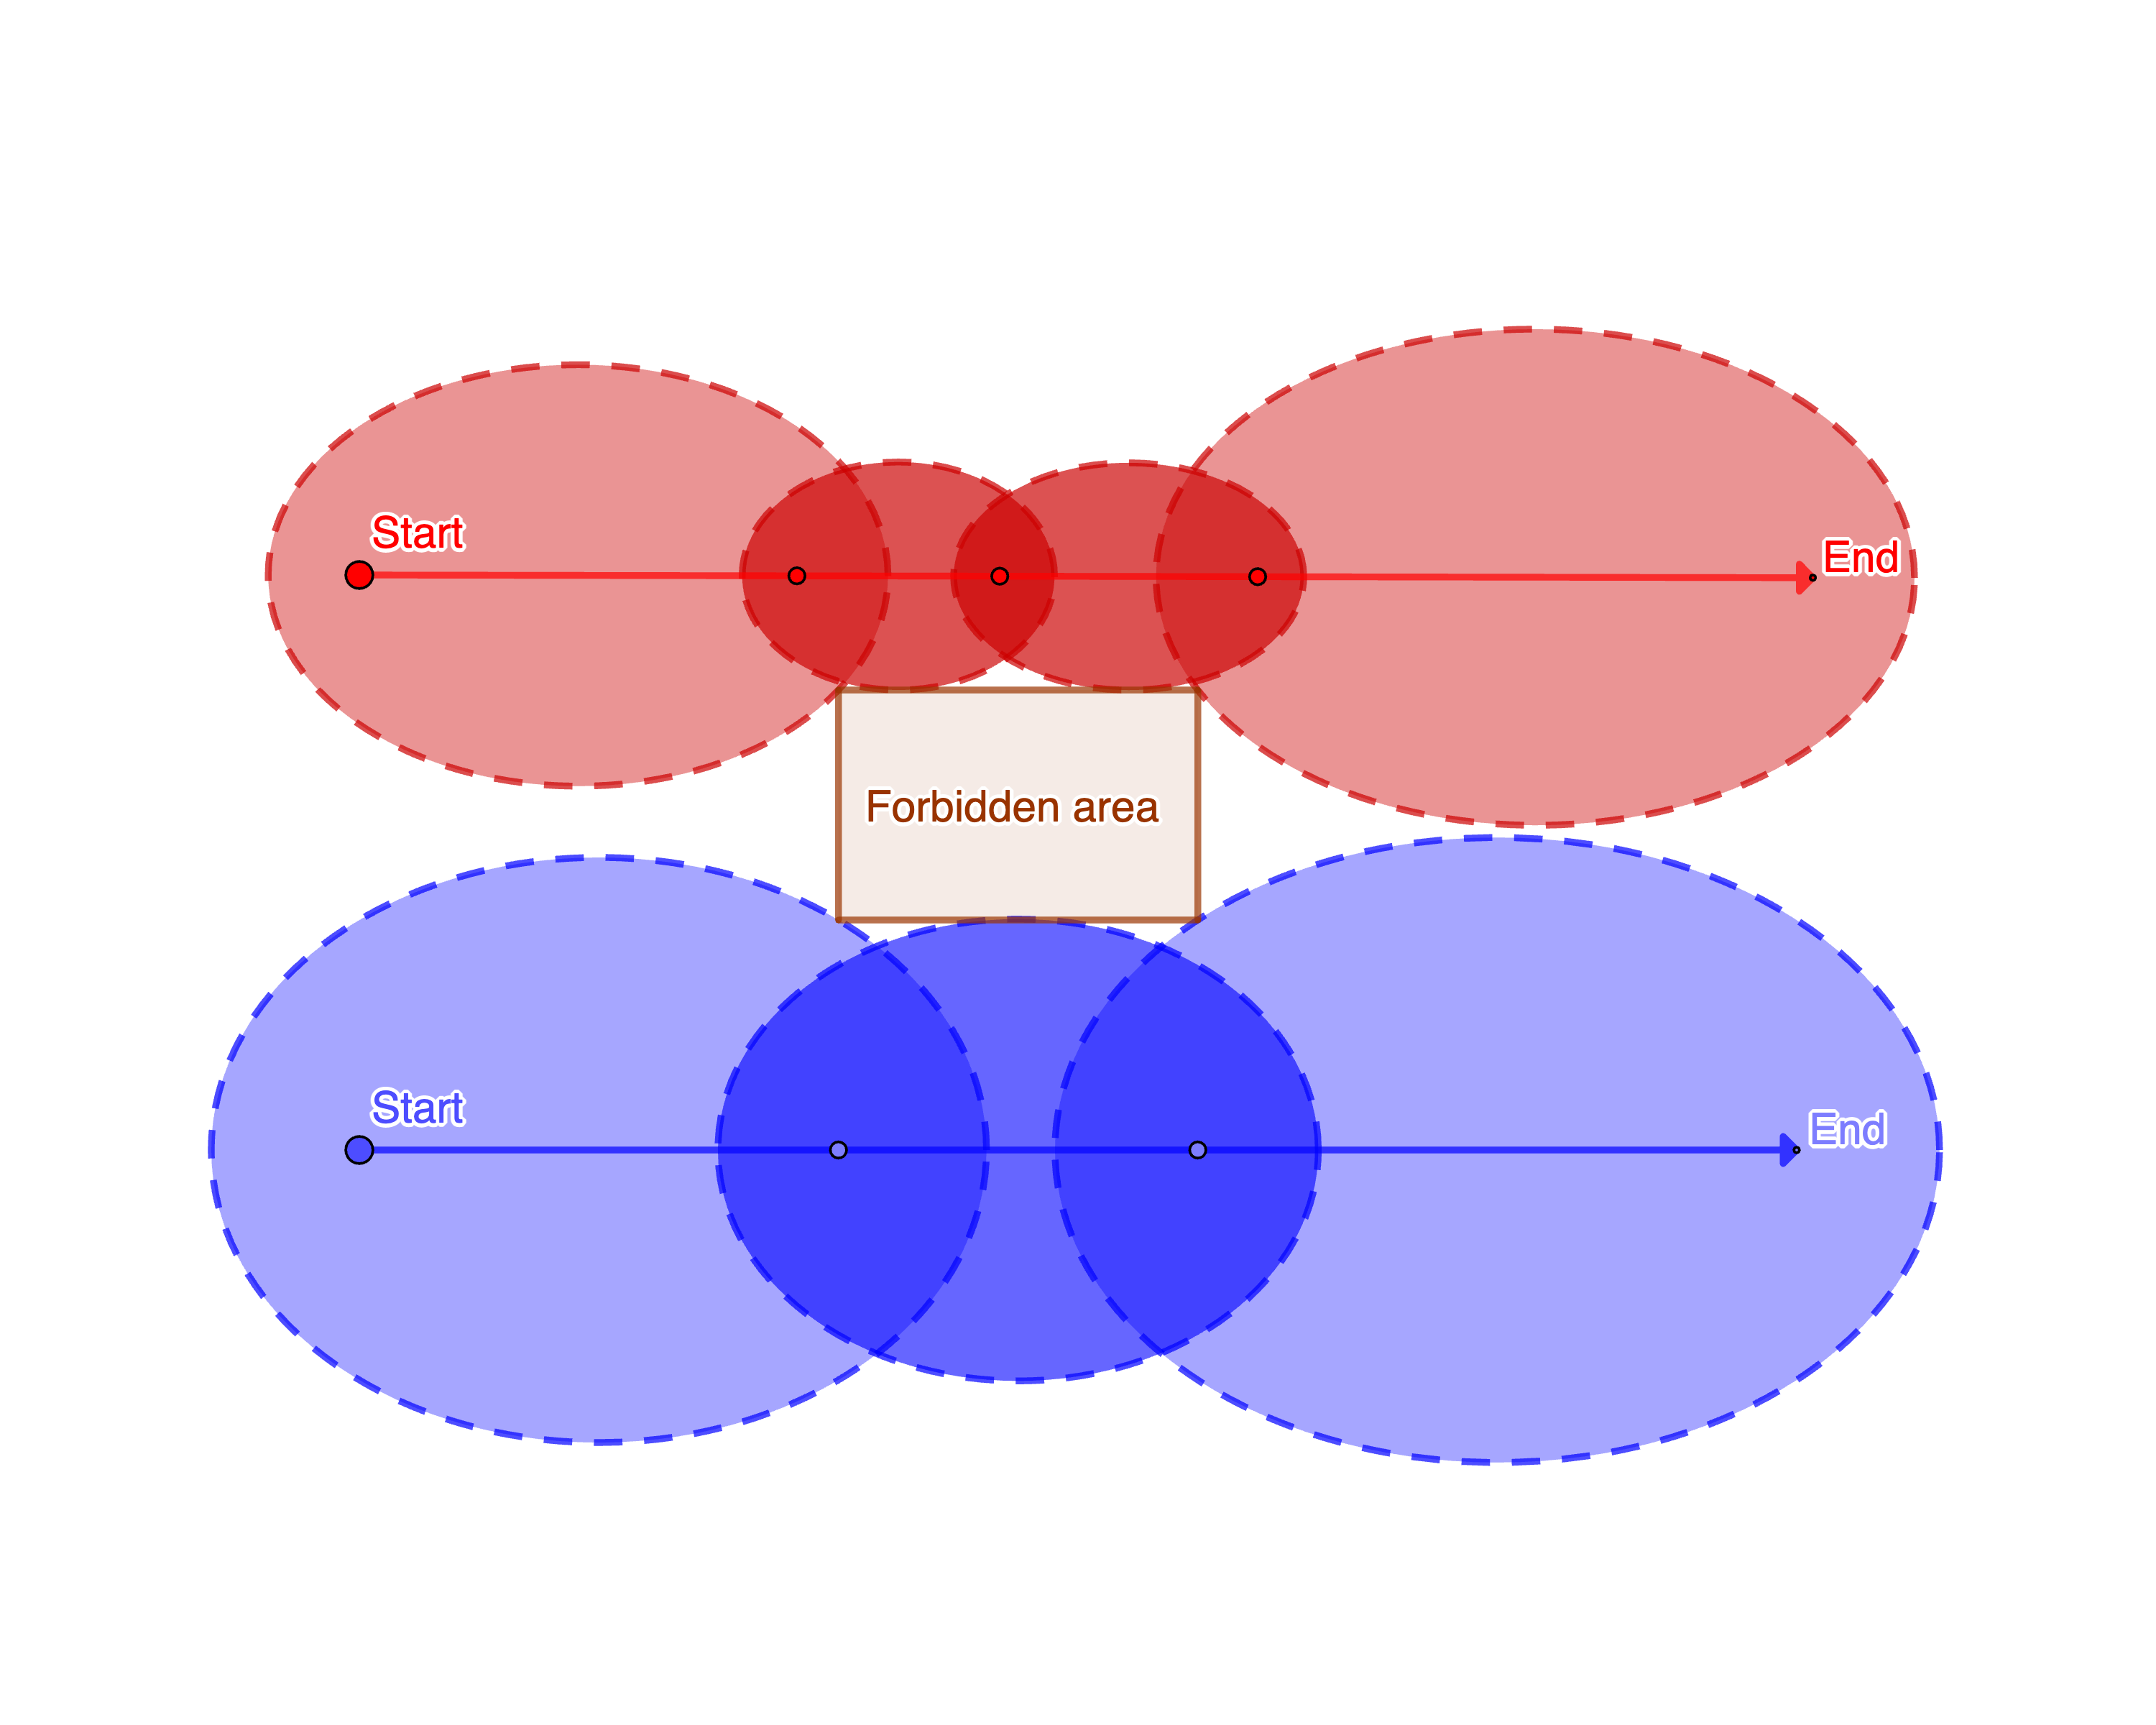
\includegraphics[width=0.45\linewidth]{SC_gen_2}}
    \caption{Checkpoint generation example}\label{fig:checkpoint-generate}
\end{figure}

\subsubsection{Cross-trajectory edges}\label{sec:cross-traj-edges}
After locating checkpoints $\union_p V_p$ for all sub-teams, we can search for cross-trajectory edges to connected all checkpoints to trajectories. Cross-trajectory edges represents feasible paths between two references trajectories that allow robots to reach a different reference trajectories and perform co-observations with the corresponding sub-teams. 
Thus, at least one end of the edges must be a security checkpoint $v_{p} \in \union_p V_p$. Additionally, assuming that only one robot is sent at a time between trajectories, the cross-trajectory edges must satisfy the reachability constraints from~\Cref{chapter:Reachability_Constraints} to ensure that no deviation to forbidden areas can be performed while switching trajectories.  

\begin{figure}[htbp]
\begin{center}
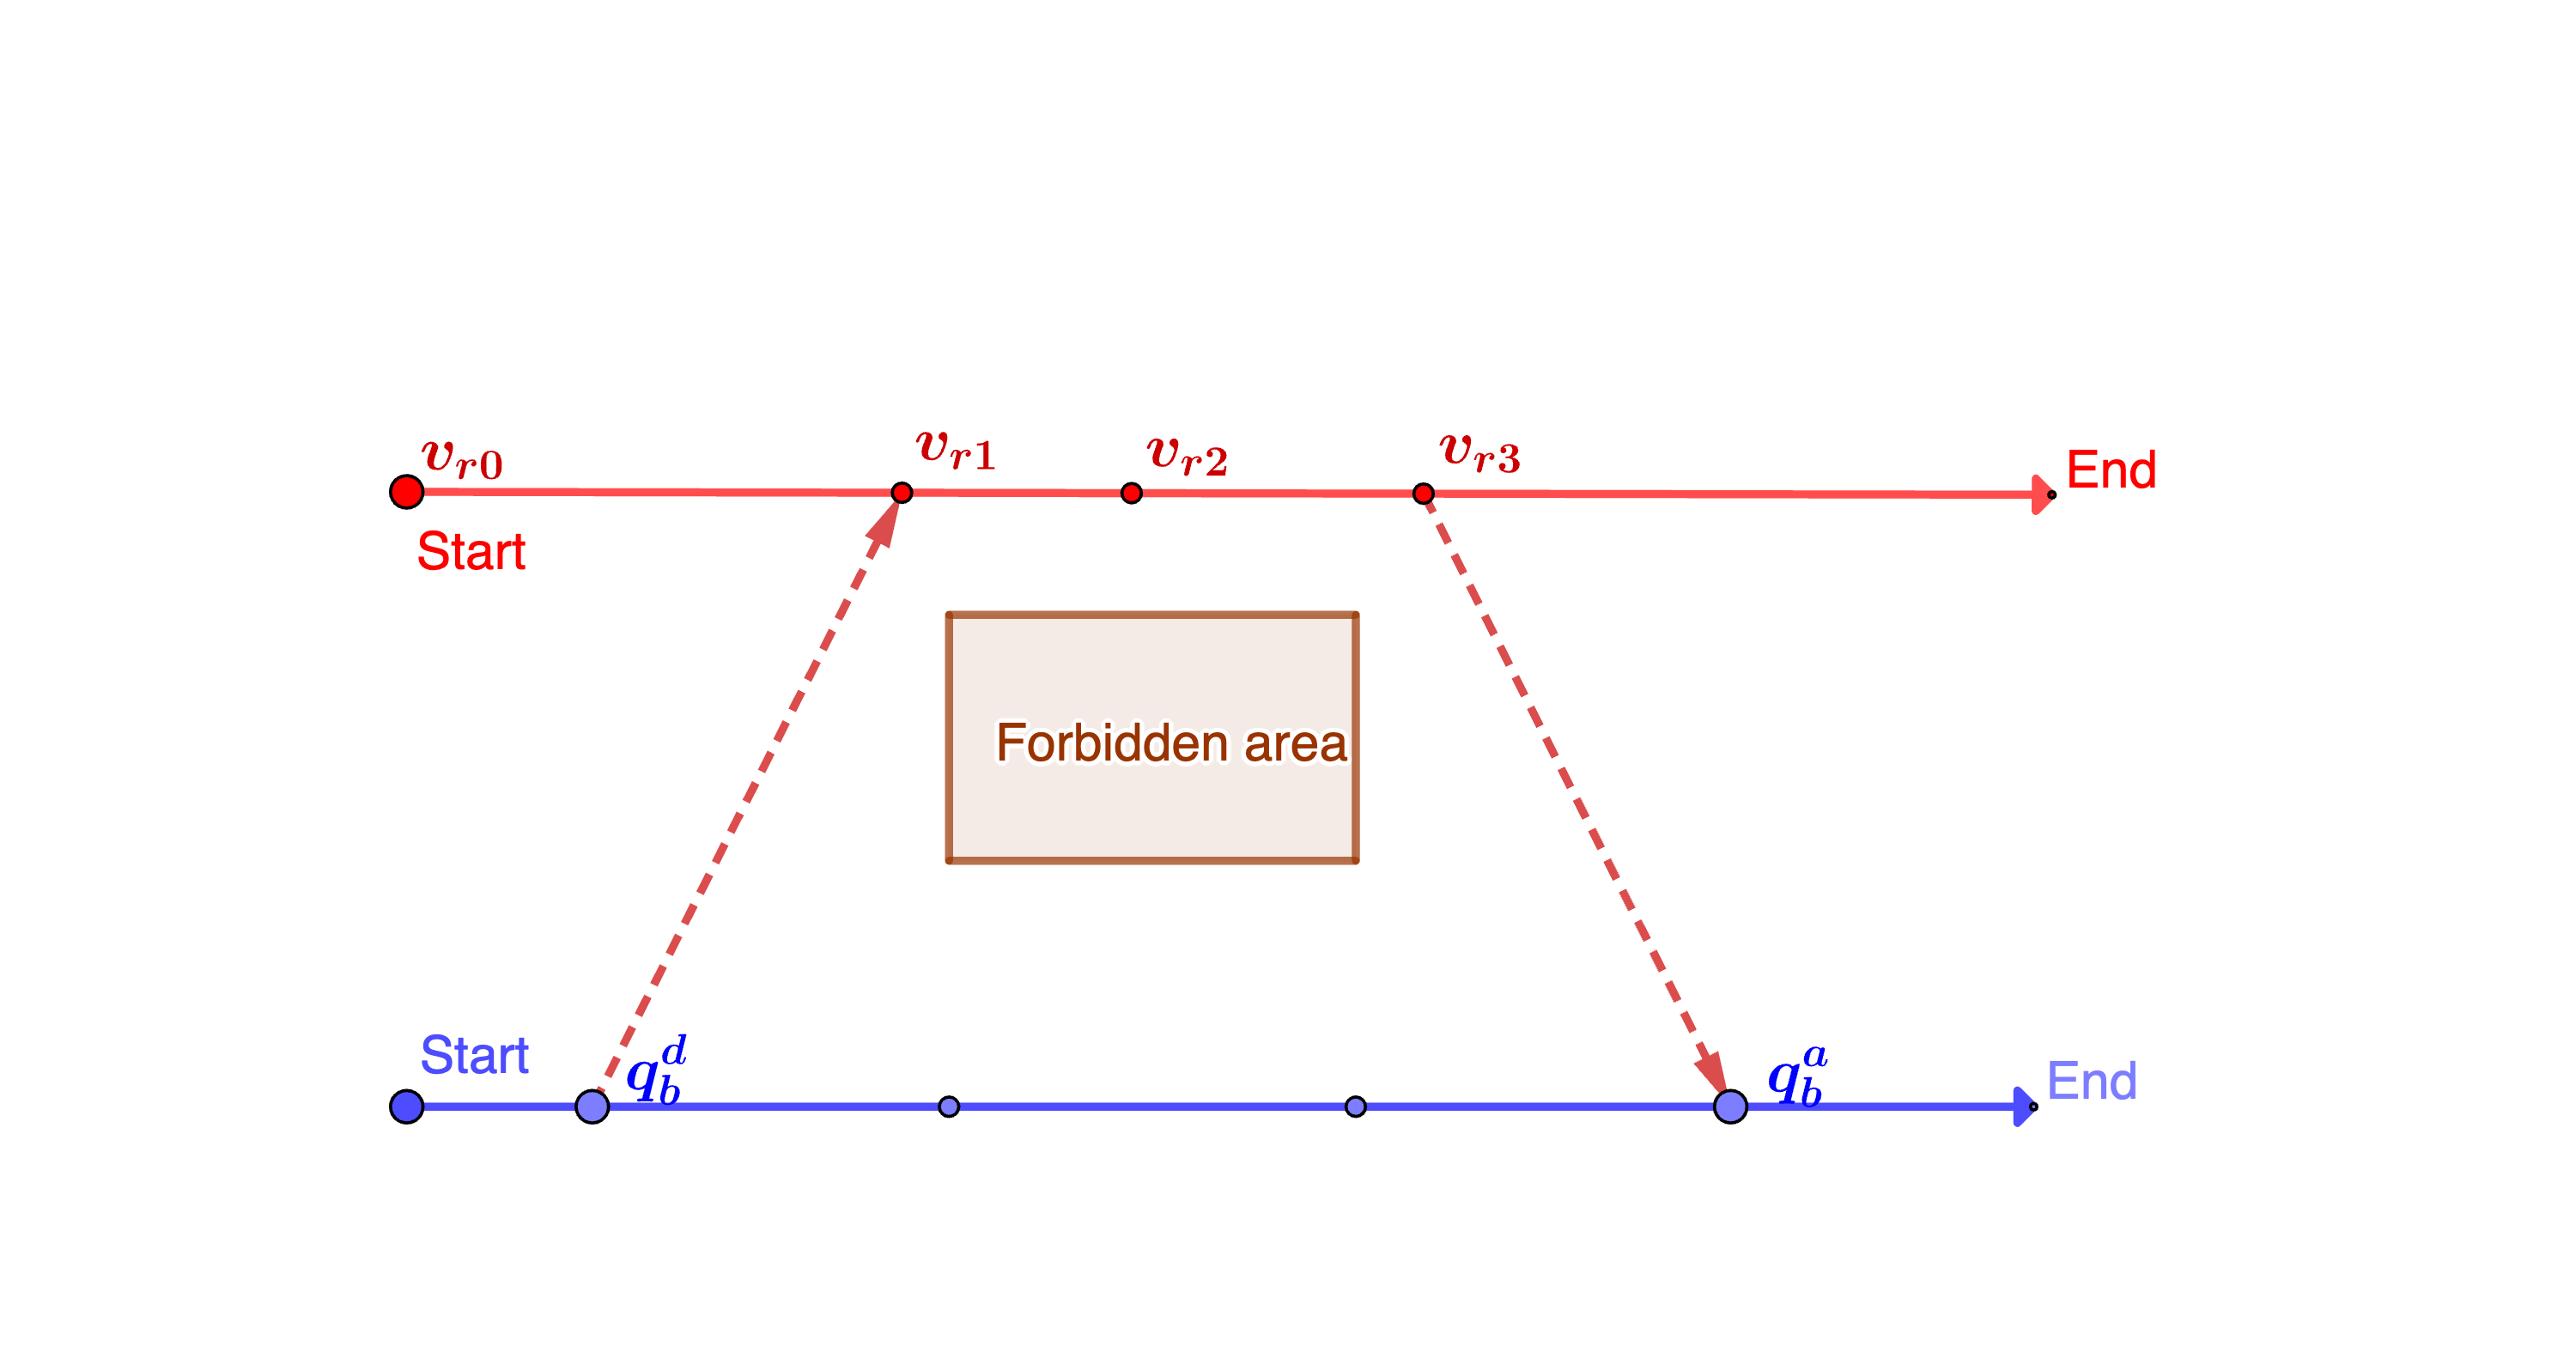
\includegraphics[width=0.6\linewidth]{two_edges}
\caption{For checkpoints of the red trajectory, latest departure node $q^{d}_{b}$ found for $v_{r1}$ and earliest arrival node $q^{a}_{b}$ found for $v_{r3}$.}
\label{fig:two-edges}
\end{center}
\end{figure}

To find cross-trajectory edges, we first find trees of feasible paths using \rrtstar{} and position information alone; we then prune these trees by considering time constraints (that consider the time needed to physically travel from one trajectory to the other while meeting other robots at the two endpoints) and ellipsoidal rechability constraints.

We search for feasible paths between each security checkpoint and all other trajectories (ignoring, for the moment, any timing constraint), as shown in \Cref{fig:RRT*} \rtron{Missing figure}. 
%Paths returned by RRT* are optimal and bidirectional.%, we can analyze the travel time and reachability for each candidate cross-trajectories, and  add these edges to the checkpoint graph if they are feasible.
More precisely, after a fixed number of  iterations, \rrtstar{}  finds all feasible, quasi-optimal paths between one security checkpoint $v_{p}=(q_{p},t_{p}) \in V_{p}$ for sub-team $\cI_p$, and $V_{r} = \{ (q_{{r}_{i}}, t_{{r}_{i}}) \}$ where  $q_{{r}_{i}} = q_{r}(t_{{r}_{i}})$ are the entire waypoints on a reference trajectories for a different sub-team $\cI_{r}$.
We can calculate the minimal travel time $t=\texttt{Cost}(q)/v_{max}$ for a robot to traverse each path. We call all nodes $v_{{r}_{i}} \in V_{r}$ \emph{arrival node}s if there exist a path between $v_{{r}_{i}}$ and $v_{p}$ with $t_{p}+t<t_{{r}_{i}}$, and the reachability ellipsoid $\mathcal{E}(q_{r}(t_{{r}_{i}}),q_{p},t_{{r}_{i}},t_{p}) \intersect F = \emptyset$. Similarly, \emph{departure node}s are defined for $v_{{r}_{i}}$ with $t_{p}>t_{{r}_{i}}+t$ and $\mathcal{E}(q_{p}, q_{r}(t_{{r}_{i}}),t_{p}, t_{{r}_{i}}) \intersect F = \emptyset$. Given a point $v_{p} \in V_{p}$, we define the \emph{latest departure node} $q_{r}(t^{d}_r)$, and the \emph{earliest arrival node} $q_{r}(t^{a}_r)$ as follows:

\begin{description}
\item[Latest departure node $q_{r}(t^{d}_r)$]: is the waypoint with the latest time $t^{d}_r$ such that a robot from sub-team $\cI_r$  can meet with robots in sub-team $\cI_p$ at $v_{p}$.
\item[Earliest arrival node $q_{r}(t^{a}_r)$]: is waypoint with the earliest time $t^{a}_r$ such that a robot from sub-team $\cI_p$ deviating from $v_{p}$ can meet with sub-team $\cI_r$.
\end{description}

For $v_{p} \in V_{p}$, latest departure node $v_{d}=(q_{r}(t^{d}_r),t^{d}_r)$ and earliest arrival node $v_{a}= (q_{r}(t^{a}_r),t^{a}_r)$, if feasible, are added to $V_{q}$. Cross-trajectory edges $(v_{p} \to v_{a})$ and $(v_{d} \to v_{p})$ are added to $E_{q}$. Examples are shown in Figure \ref{fig:two-edges}. Full algorithm is shown in Algorithm \ref{alg:cross-trajectory-edges}.

\begin{algorithm}
\caption{Cross-trajectory edges generation}\label{alg:cross-trajectory-edges}
\begin{algorithmic}
\Procedure{CrossTrajectoryEdges}{$V$}
\State $V_{q} \gets V$; $E_{q}\gets 0$;
\ForAll {$v\in V$}
	\ForAll{$\vq_{r}$ that $\cI_{r} \neq \cI_{v}$}
		\State $V_{q},E_{q} \gets \textsc{AddEdges} (q_{v}, \vq_{r}, V_{q}, E_{q}) $;
	\EndFor
\EndFor
\State \Return $V_{q}, E_{q}$
\EndProcedure
\Procedure{AddEdges}{$q_{v}, \vq_{r}, V_{q},E_{q}$}
\State $t^{d}_r \gets -\infty $; $t^{a}_r \gets \infty$;
\State $\cV_{goal}=RRT^*(q_{v}, \vq_{r})$;
    \ForAll{$ q \in \cV_{goal} $ that $\texttt{Parent}(q)\neq \emptyset $}
        \If{$\texttt{Cost}(q)/ v_{max} < t_{q}-t_{v}$ and $\cE(q, v_{p},t_{q}, t_{v_{p}})\union F = \emptyset$}
        		\If{$t_{q}<t^{a}_r$}
			\State $t^{a}_r \gets t_{q}$;
		\EndIf
        \ElsIf{$\texttt{Cost}(q)/ v_{max} < t_{v} - t_{q}$ and $\cE(q, v_{p},t_{q},t_{v_{p}})\union F = \emptyset$}
        		\If{$t_{q}>t^{d}_r$}
			\State $t^{d}_r \gets t_{q}$;
		\EndIf
        \EndIf
    \EndFor
    \If{$t^{d}_r \neq -\infty $ and $t^{a}_r \neq \infty$}
    \State $v_{a} \gets (q(t^{a}_r),t^{a}_r)$; $v_{d} \gets(q(t^{d}_r), t^{d}_r)$;
    \State $V_{q}\gets V_{q} \union v_{a}$; $V_{q}\gets V_{q} \union v_{d}$;
    \State $E_{q}\gets E_{q} \union (v_{p} \rightarrow v_{a})$; $E_{q}\gets E_{q} \union (v_{d} \rightarrow v_{p})$
    \EndIf
    \State \Return $V_{q},E_{q}$
    \EndProcedure
   \end{algorithmic}
\end{algorithm}

\subsubsection{In-trajectory edges}\label{sec:Graph-intro}

%With vertices $V_{q}$ and cross-trajectory edges $E_{q}$ found in Algorithm \ref{alg:cross-trajectory-edges}, we can construct a security graph $G_{q}$. 
All checkpoints $V_{q}$ found in Section~\ref{sec:security-checkpoint} and \ref{sec:cross-traj-edges}, can be divided by the corresponding sub-team and sorted in ascending order of time into $N_{p}$ subsets $V_{p}=\{v^{p}_{0}, v^{p}_{1}, \dots , v^{p}_{T}\}$ where $p\in \{1,\dots, N_{p}\}$. Consecutive edges in the same subset are added to $E_{q}$ as in-trajectory edges $(v^{p}_{i}\rightarrow v^{p}_{i+1} )$. Example are shown in Figure \ref{fig:security-graph-generate}.
\begin{figure}[htbp]
\begin{center}
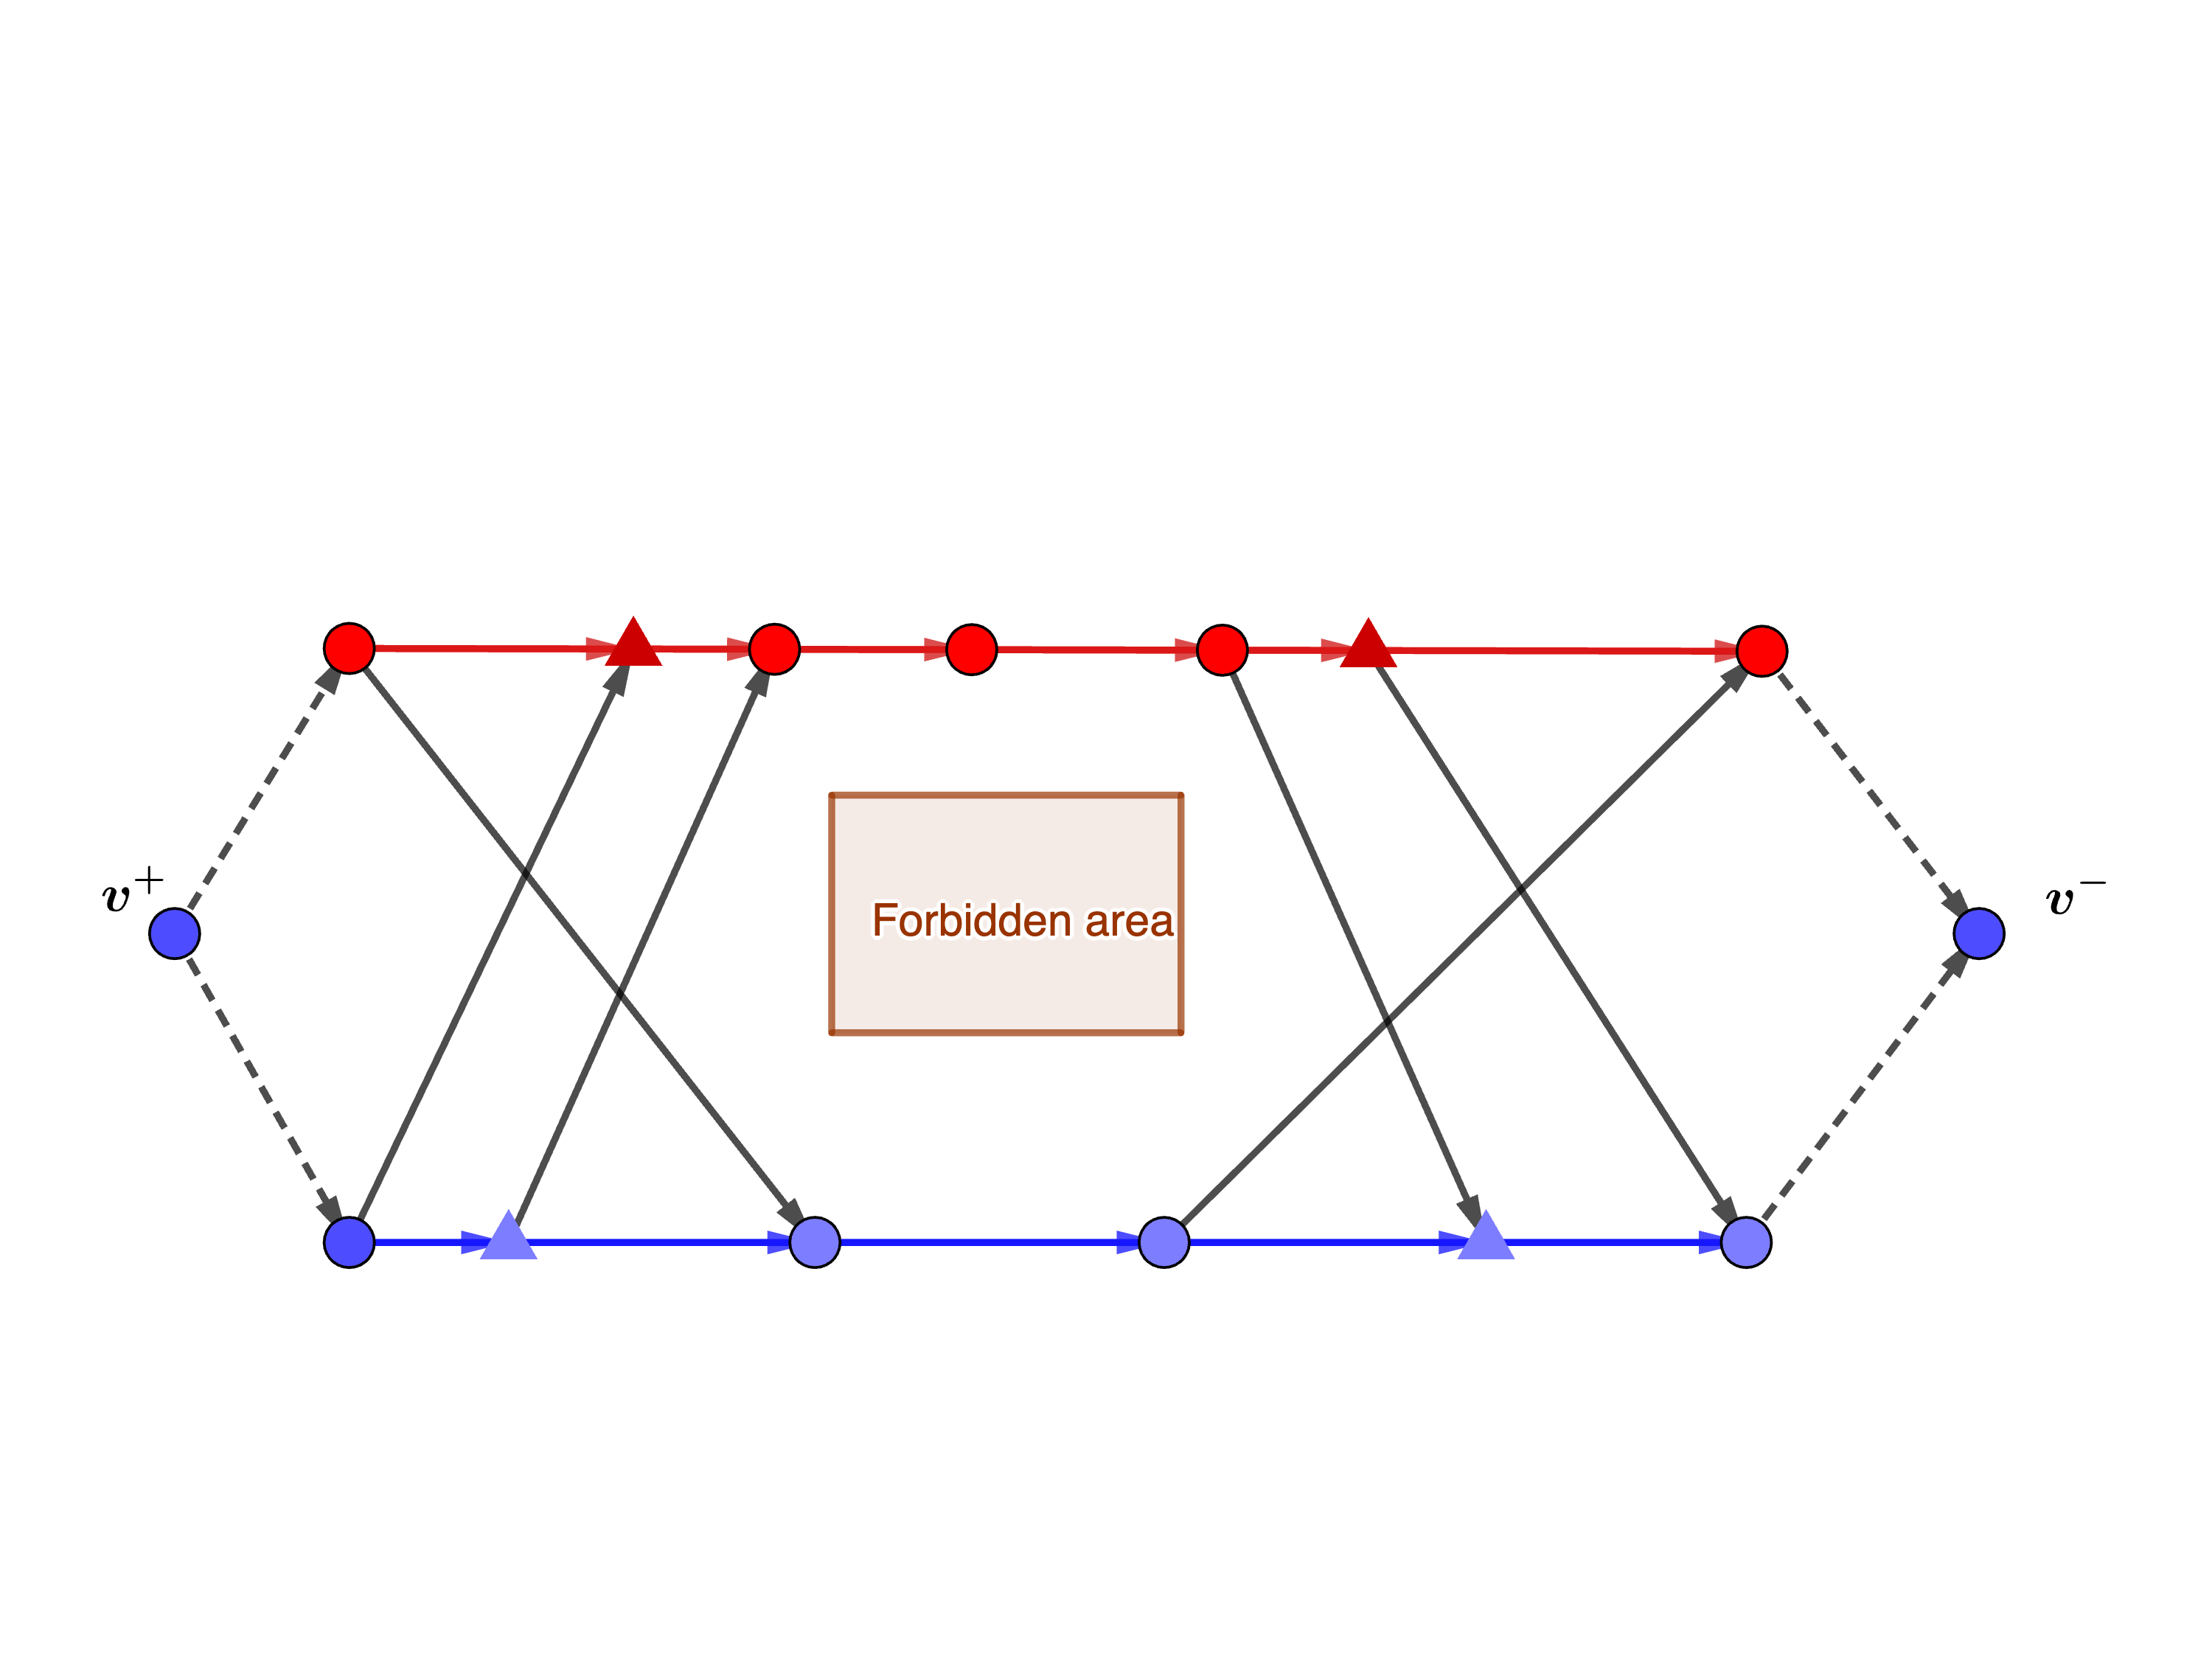
\includegraphics[width=0.6\linewidth]{security_graph}
\caption{Example of a two trajectory security graph. Round vertices are checkpoint generated through the heuristic search and triangle vertices are added with the cross-trajectory edges. Additional virtual source $v^{+}$ and sink $v^{-}$ is used later in planning problem.}
\label{fig:security-graph-generate}
\end{center}
\end{figure}

%For convenience, we use $|V_{q}|$ and $|E_{q}|$ to denote the cardinality of the sets $V_{q}$ and $E_{q}$ 

\subsection{Co-observation planning problem}
In this section, we describe in detail how to formulate the cross-trajectory planning problem as a network flow problem, and solve it using mixed-integer linear programs (MILP). We assume that there are always \emph{reference robot}s in each sub-team following the reference trajectory.  We want to plan the routes for additional \emph{cross-trajectory robots} to perform co-observation with the reference robots. 

To formulate the planning problem as a network multi flow problem, we augment the checkpoint graph $G_{q}$ to a flow graph $G=(V, E)$. The vertices of the new graph are defined as $V= V_{q} \union \{v^{+},v^{-}\}$,  a \emph{virtual source} $v^{+}$ and a \emph{virtual sink} node $v^{-}$ are added to $V$. The edges of the new graph are defined as $ E = E_{q} \union \{( v^{e}_{p},v_{-})\}_{p} \union \{(v_{+},v^{0}_{p})\}_{p}$, where directed edges are added to $E$ from $v^{+}$ to all the start vertices, and from all end vertices to $v^{-}$, with $v^0_p$ and $v^e_p$ representing the start and end vertices of sub-team $\cI_p$.

Assume that all the robots starting from the virtual source $v^{+}$ and end in the virtual sink $v^{-}$. Each robot may move from vertex $v_{i}$ to $v_{j}$ if $(v_{i},v_{j})\in E_{q}$. The path of a robot $k$ can be represented as a flow vector $\vf^{k} = \{ f^{k}_{ij} \}$, where $f^{k}_{ij} \in \{1,0\}$ is an indicator variable representing whether robot $k$'s path contains the edge $(v_{i},v_{j})$. As required by the security guarantee, reference robots must be seen by at least one surveillance robot at every checkpoint. Thus, the planning problem can then be formulated as a path cover problem on $G_{q}$, i.e., as finding a set of paths $F=[\vf_{1},\dots, \vf_{\cK}]$ for cross-trajectory robots such that every checkpoint in $V_{p}$ is included in at least one path in $F$. Additionally, to encourage the robots' exchange between different sub-teams, cross-trajectory co-observations are preferred compared to co-observation within the same team. This is achieved with the weights for edges $(v_{i},v_{j})\in E$ defined as:
\begin{equation}
	w_{i,j}=\begin{cases}
	-w_{t} & \cI_{v_{i}}=\cI_{v_{j}}, (v_{i},v_{j})\in E_{q}\\
	w_{c} & \cI_{v_{i}} \neq \cI_{v_{j}}, (v_{i},v_{j})\in E_{q}\\
	0 &  (v_{i},v_{j})\in E / E_{q} 
	\end{cases}
\end{equation}
where $w_{c} > w_{t}$. 

With the formulation above, the planning problem can be written as an optimization problem, where we want to balance between the co-observation performance and total number of flows (cross-trajectory robots) needed. For convenience, we use $(ij)$ to represent the edge $(v_{i},v_{j})$, and $(+i)$ to represent the edge $(v^{+},v_{i})$.

 \begin{subequations} \label{eq:flow-coverage-problem}
     \begin{align}
        \min & \sum^{\cK}_{k} \sum_{(+i)\in E} f^{k}_{+i} - \rho \sum^{\cK}_k \sum_{(ij)\in E} w_{ij} f^k_{ij} \label{eq:flow-cost}\\
        s.t. & \sum_{\{h:(hi) \in E\}}f^k_{hi}=\sum_{\{j:(ij) \in E\}}f^k_{ij},  \forall k,\forall v \in V_{q} / \{v^{+}, v^{-}\}  \label{eq:FlowBalanceConstraint}\\
        & \sum^{\cK}_k\sum_{\{i:(ij)\in E \}} f^k_{ij} \geq 1, \forall v_{j} \in \{V^{s}_{p}\} \label{eq:FlowCoverage}\\
        & f^k_{ij} \in \{0,1\} ,  \forall (ij)\in E\label{eq:SingleFLowCapacity}
     \end{align}
 \end{subequations}

The first term in \ref{eq:flow-cost} is total outgoing flow from the source $v^{+}$ while the second term is the total cost of all flows which represents the overall co-observation performance (defined as the total number of cross-trajectory edges taken by all flows beyond the regular trajectory edges). The constant $\rho$ is a penalty parameter manually elected to balance between two terms in the cost function. The constraint \eqref{eq:FlowBalanceConstraint} is the flow conservation constraint, which ensures that the amount of flow entering and leaving a given node $v$ is equal (except for $v^{+}$ and $v^{-}$). The constratin \eqref{eq:FlowCoverage} is the flow coverage constraints, which ensures that all security checkpoints $ \{V^{s}_{p}\}$ have been visited by at least one flow (robot). Since the security graph $G_{q}$ is acyclic, this problem is in complexity class $P$, and can be solved in polynominal time \cite{ntafos1979path}. 

\subsection{Co-observation performance}
Notice that problem \eqref{eq:flow-coverage-problem} is guaranteed to have a solution for $\cK=N_{p}$ where all $\cK$ robots follows the reference trajectory ($f^{k}_{ij}=1, \forall \cI_{v_{i}}=\cI_{v_{j}}=k$).  Additionally, for a fixed number of robots $\cK \geq N_{p}$, it is possible to have a subset of flows $F_{\cE} \in F$ that is empty, i.e. $f_{ij}=0, \forall (v_{i},v_{j})\in E$, $f\in F_{\cE}$, these flow will not increase the cost and will not have any impact on the solution.  
The trade-off between the number of surveillance robots used, and the overall security performance is a critical consideration in this case. Increasing the number of robots generally contributes to improved security by enabling more cross-trajectory co-observations. However, adding more robots can lead to diminishing returns, as the benefits gained from additional robots may be counterbalanced by increased complexity and coordination challenges. To capture this trade-off, the penalty parameter $\rho$ in the cost function \ref{eq:flow-cost} allows us to fine-tune the balance between the number of robots employed and the desired task performance. By optimizing this parameter, we can strike a suitable equilibrium between security enhancement and operational efficiency.

To find such tradeoff, we employ an iterative approach. We start with $\cK=1$ and gradually increase it until $F$ contains a empty flow. This indicates that the performance can no longer be improved by adding more robots. To ensure that the value of $\cK$ does not grow unbounded, penalty parameter $\rho$ need to ensure that the second term for a single flow in \eqref{eq:flow-cost} $ \rho \sum_{(ij)\in E} w_{ij} f^k_{ij}$ is always smaller than $1$.

\subsection{Result and simulation}
In this section, we test the proposed method starting from the results in Figure \ref{fig:trajectories-more-constraint}, where three trajectories are provided for the map exploration task with no security related constraints (co-observation schedule and reachability). We use the same environment and dynamic setup, where we have a $10m\times10m$ task space, two forbidden regions (two rectangles in  \ref{fig:trajectories-more-constraint}) and robots with a max velocity of $0.5m/dt$.

\begin{figure}[t]
\begin{center}
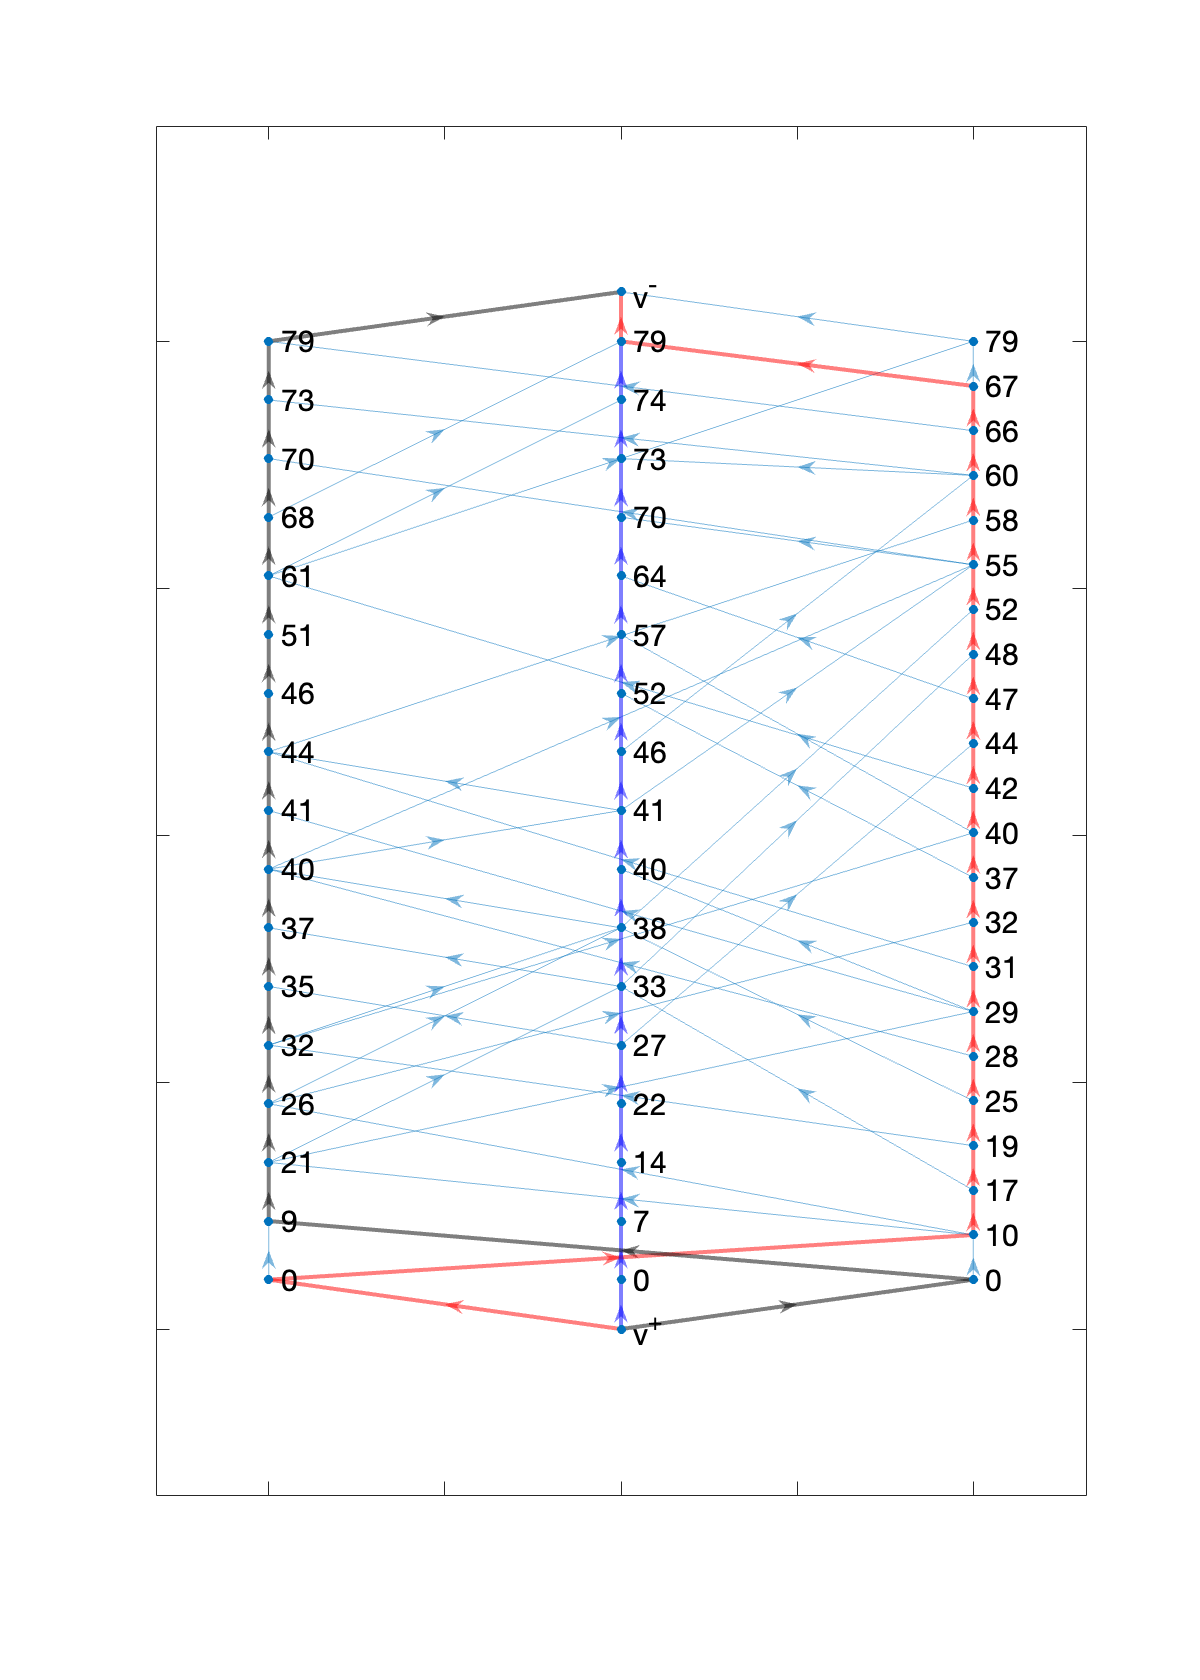
\includegraphics[width=0.4\linewidth]{graph_flow_result_3}
\caption{Security Graph and result for 3 flows}
\label{fig:security-graph-3-flow}
\end{center}
\end{figure}

\begin{figure}[htbp]
\begin{center}
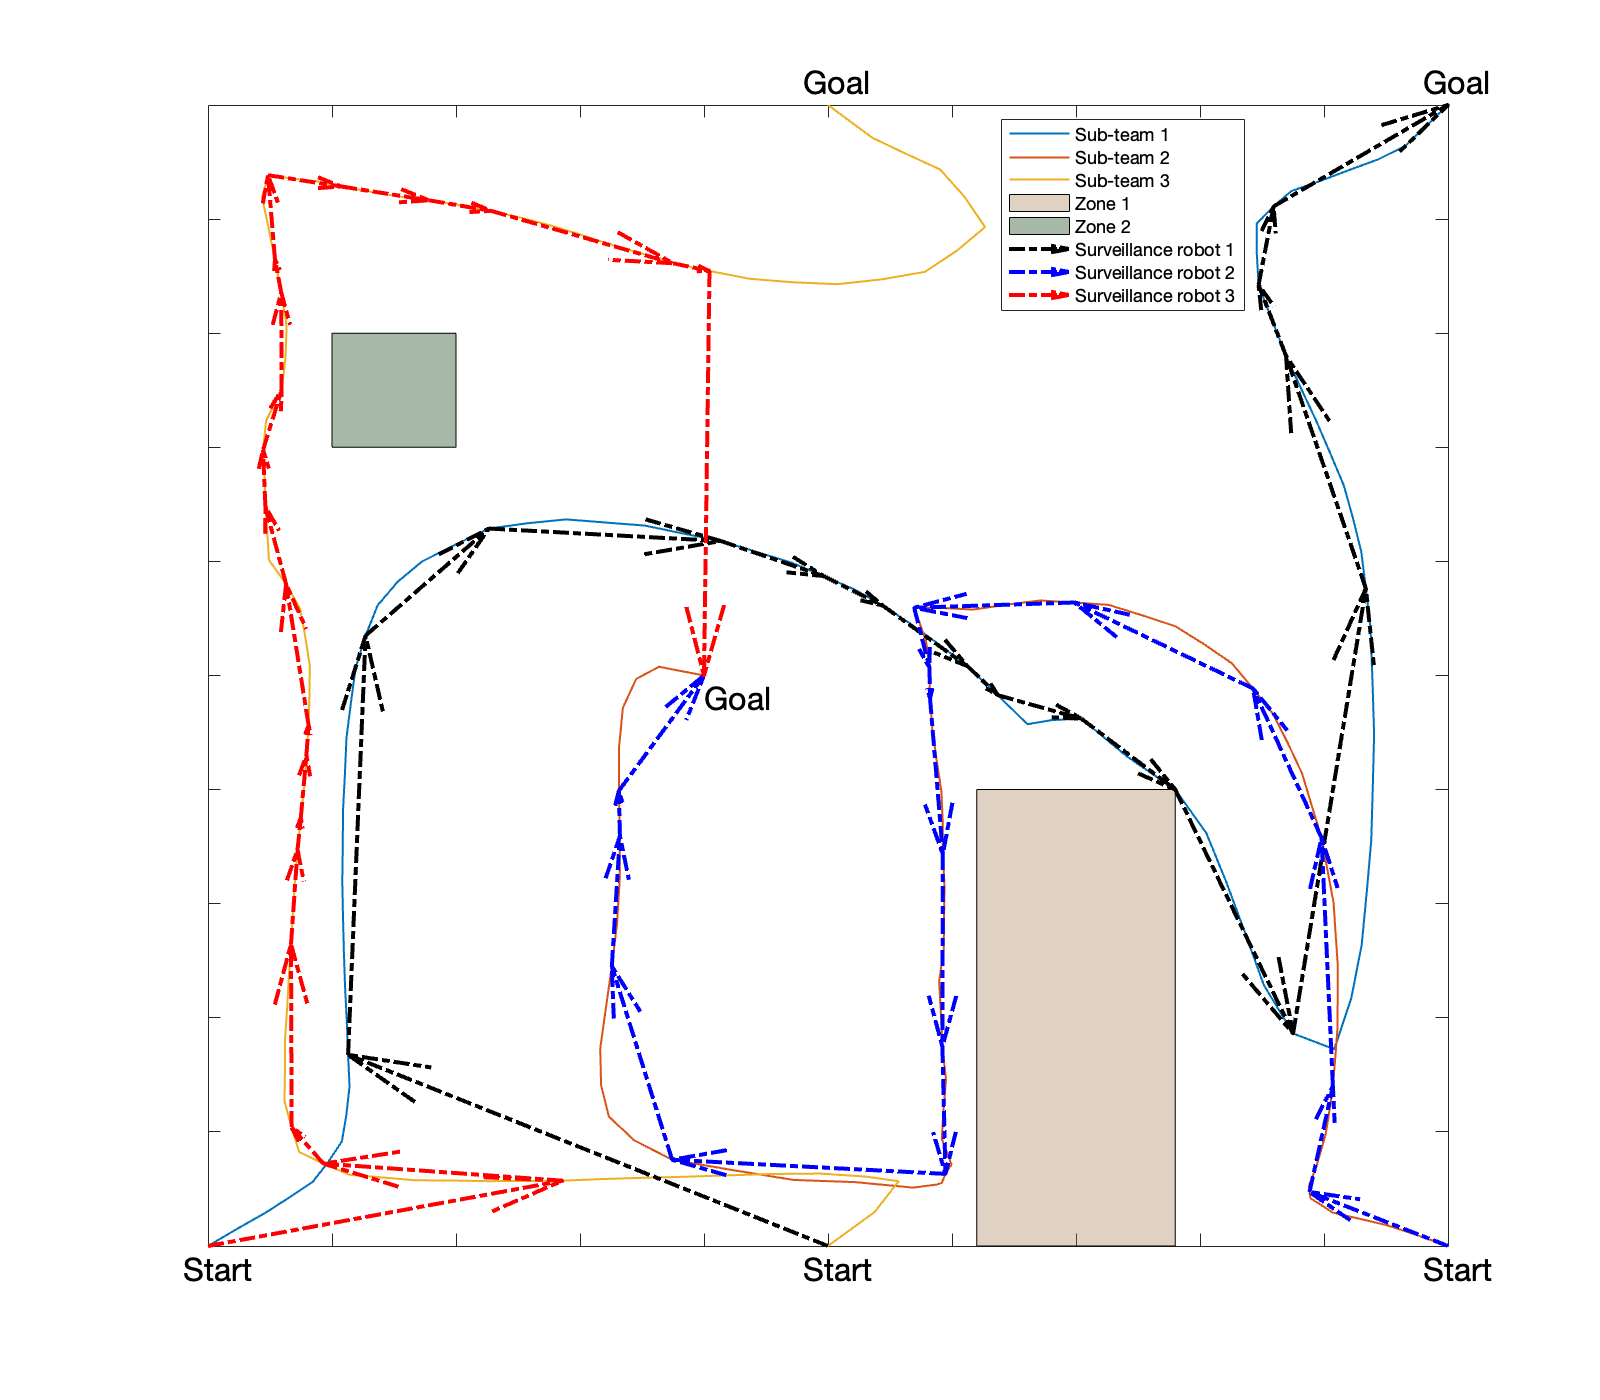
\includegraphics[width=0.6\linewidth]{3_flow_result}
\caption{Result of 3 surveillance agents' plan in workspace}
\label{fig:workspace-3-flow}
\end{center}
\end{figure}

We start by adding a total of $\cK=3$ surveillance robots into the workspace using the parameters $w_{c}=10$, $w_{t}=1$ and $\rho = 0.01$. The three trajectories are transformed into the graph $G$ shown in Figure \ref{fig:security-graph-3-flow}, where the number on each vertex $v_{i}$ represents the corresponding time $t_{i}$. Vertices in each column belong to the same trajectory, and edges across different columns are cross-trajectory edges. 

The flows derived from the solution of the optimization problem \eqref{eq:flow-coverage-problem} are highlighted in the graph. The planning result in the workspace is shown in \ref{fig:workspace-3-flow} as dash-dotted arrows with the same color used for each flow in \ref{fig:security-graph-3-flow}. Notice that flows represent the robot co-observation plan instead of actual robots, such that the red flow, for example, shows that the sub-team 2 is expecting a robot from sub-team 1, departing at $t=0$ and arriving at $t=10$, and needs to send a robot (not necessarily the same one received from sub-team 1) to sub-team 3, departing at $t=67$ and arriving at $t=79$. This plan is not ideal in terms of our security criteria since co-observations happens between the same pair of surveillance robot and sub-team for the majority of the time with only three cross-trajectory edges that are covered.

\begin{figure}[t]
\begin{center}
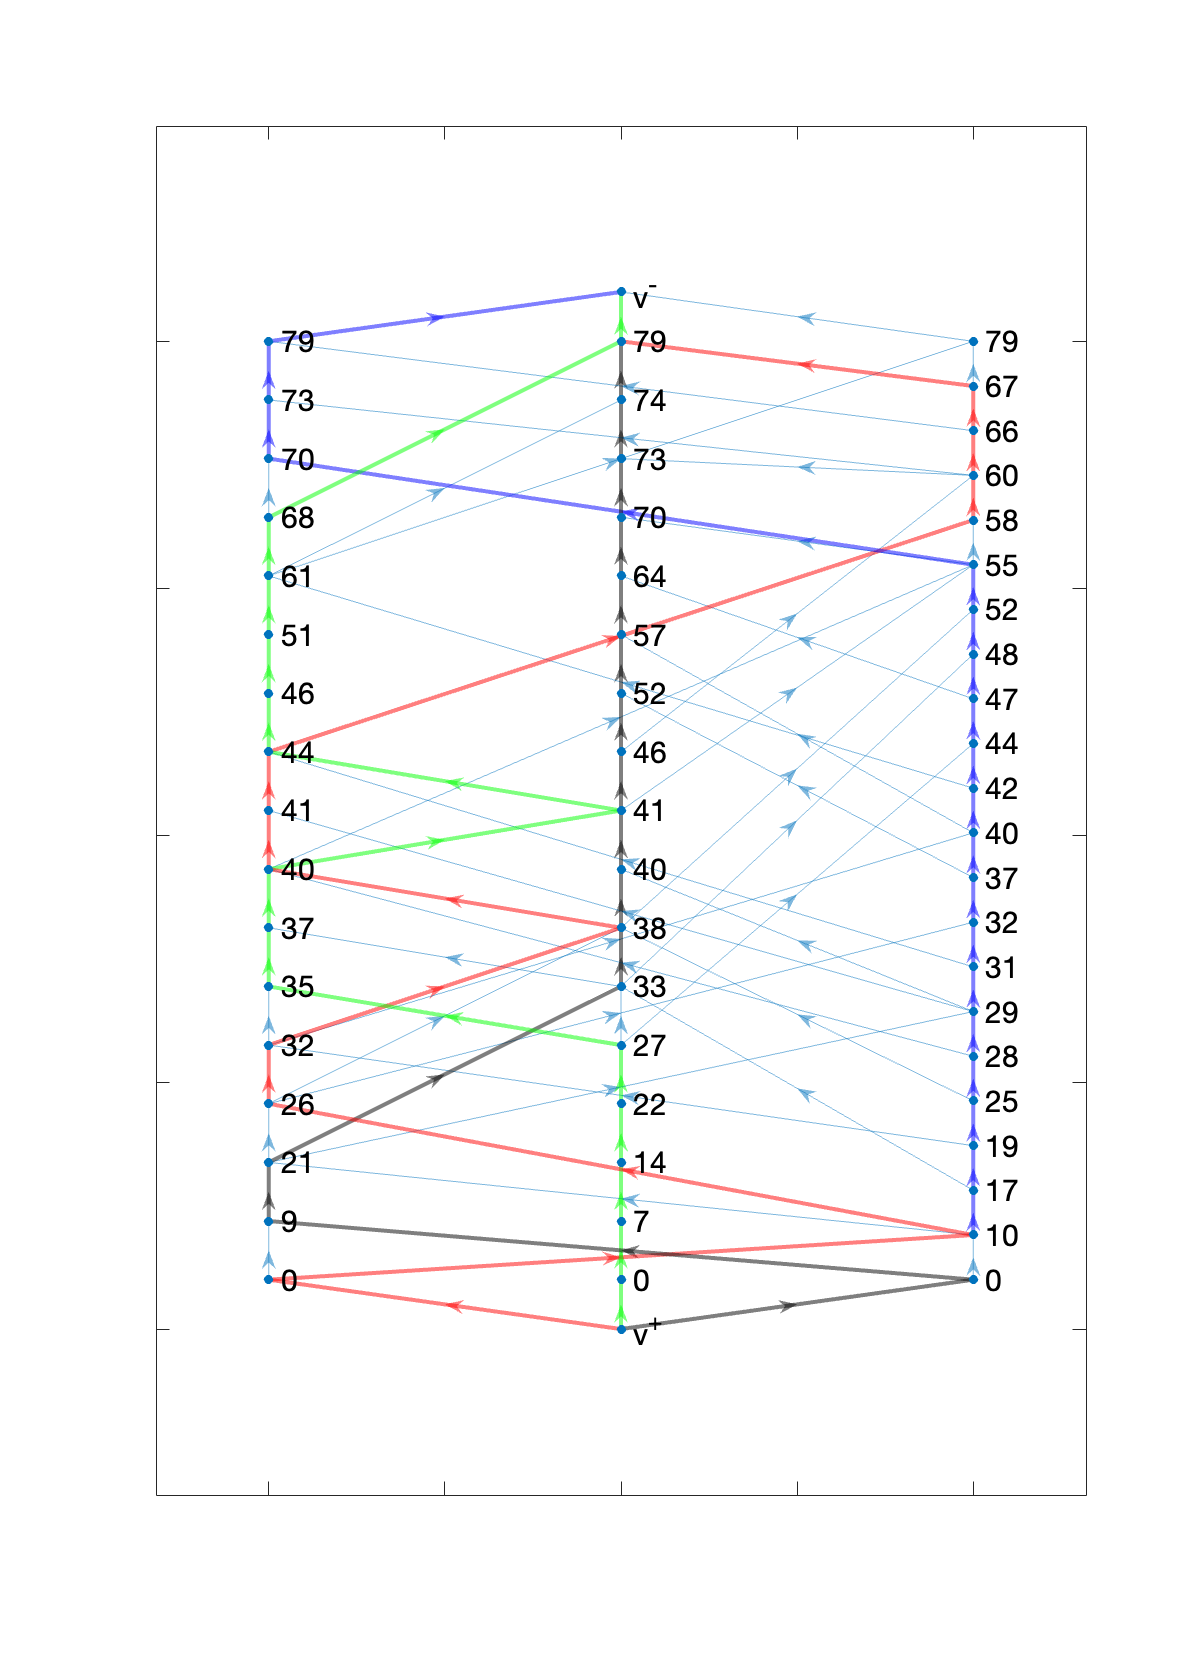
\includegraphics[width=0.4\linewidth]{graph_flow_result_4}
\caption{Security Graph and result for 4 flows.}
\label{fig:security-graph-4-flow}
\end{center}
\end{figure}

\begin{figure}[htbp]
\begin{center}
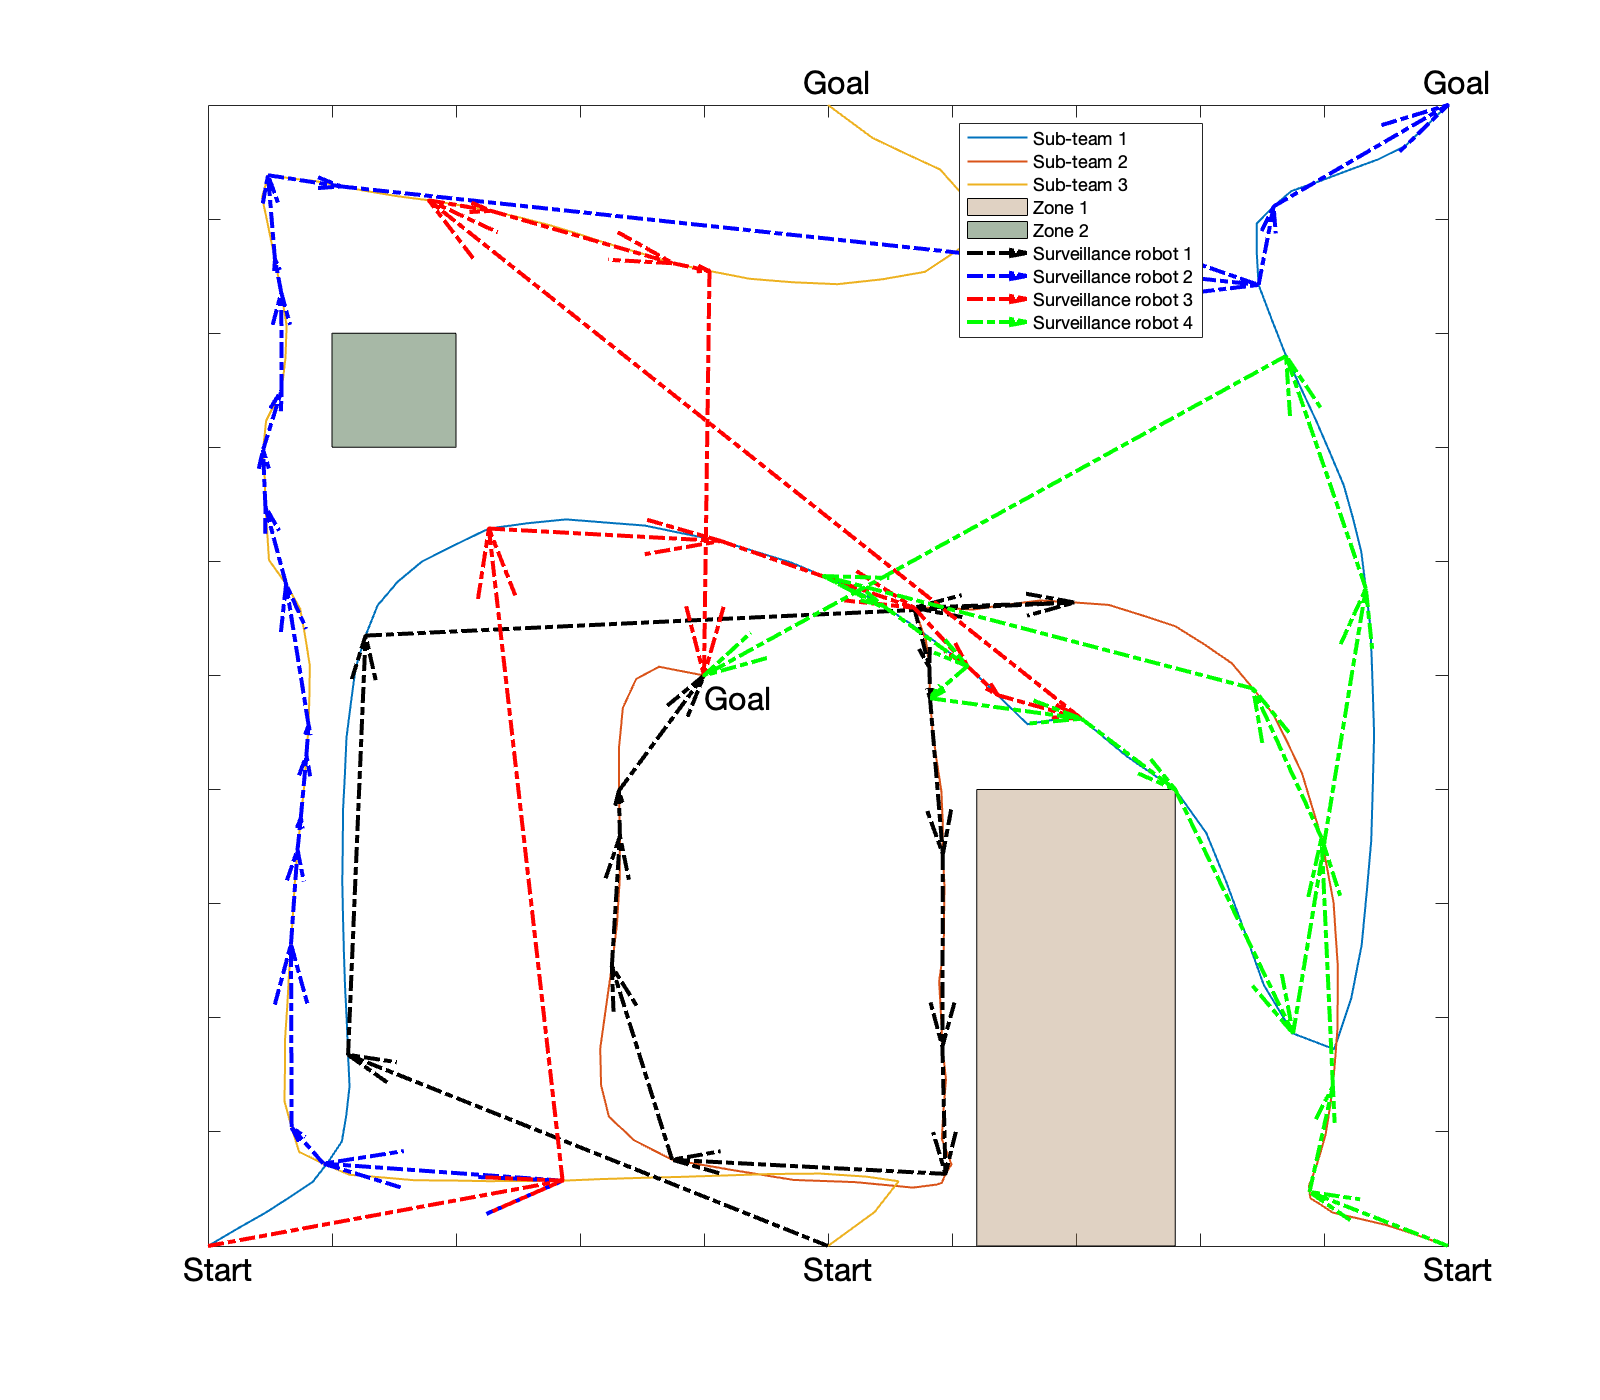
\includegraphics[width=0.6\linewidth]{4_flow_result}
\caption{Result of 3 surveillance agents' plan in work space.}
\label{fig:workspace-4-flow}
\end{center}
\end{figure}

For the case where $\cK=4$, the results are shown in Figure \ref{fig:security-graph-4-flow}-\ref{fig:workspace-4-flow}. With one additional robot added, there are significant increase in the total cross-trajectory edges covered, and sub-teams performs co-observation with different robots during the task period.

If we further increase $\cK>4$, we do not get a better result; instead, the planner will generate 4 flows with the rest $\cK-4$ flows empty.

\begin{figure}[htbp]
\begin{center}
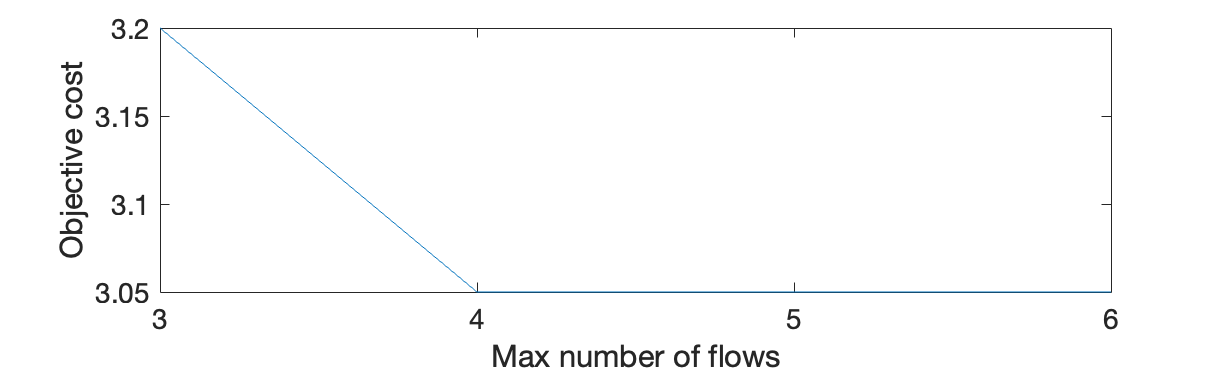
\includegraphics[width=0.6\linewidth]{nflow_vs_cost}
\caption{Plan reach optimality when $\cK=4$, further increase of $\cK$ does not increase the cost of objectives.}
\label{fig:flow-n-vs-cost}
\end{center}
\end{figure}

\section{Summary}
In this paper, we provide a method to enhance the security of a multi-robot system without sacrificing the performance. This is done by introducing additional robots to perform cross-trajectory co-observations by traveling between different trajectories. We model the unsecured multi-robot trajectories as a checkpoint graph by identifying checkpoints that requires observation and cross-trajectory paths that can safely access the checkpoints from different trajectories. We have shown that the co-observation planning problem across different trajectories can be transformed into a multi flow problem on the graph, and that we can find the minimal number of robot needed to finish the co-observation task.

\appendix


\subsection{Proof of proposition \ref{prop:HProperty}} \label{proof:HProperty}
    For subclaim~\ref{it:orthonormality}:
    \begin{equation}
      H\transpose H=H^2=4uu\transpose u u\transpose - 4uu\transpose +I^2=I,
    \end{equation}
    since $u\transpose u=1$.

    For subclaim~\ref{it:determinant}, let $U=\bmat{u & u^\bot_{1},u^\bot_{2}}$, where $u^\bot_{1},u^\bot_{2}$ are two orthonormal vectors such that $I=UU\transpose=uu\transpose + u^\bot_{1}(u^\bot_{1})\transpose+u^\bot_{2}(u^\bot_{2})\transpose$; then, substituting $I$ in \eqref{eq:H definition}, we have that the eigenvalue decomposition of $H$ is given by
    \begin{equation}
      H=U\diag(1,-1,-1) U\transpose.
    \end{equation}
    Since the determinant of a matrix is equal to the product of the eigenvalues, $\det(H)=1$.

    For subclaim~\ref{it:transformation}, first note that $Hu=2uu\transpose u - u=u$.
    It follows that the sum of $\nu_\cF$ and $\nu_\cE$ is invariant under $H$:
    \begin{equation}\label{equ:H(u1+u2)}
      H(\nu_\cF+\nu_\cE)=H u \norm{\nu_\cF+\nu_\cE}
      = u\norm{\nu_\cF+\nu_\cE} =\nu_\cF+\nu_\cE,
    \end{equation}
    and that their difference is flipped under $H$:
    \begin{equation}\label{equ:H(u1-u2)}
      H(\nu_\cF-\nu_\cE) = 2uu\transpose (\nu_\cF-\nu_\cE) - (\nu_\cF-\nu_\cE)^2 = -(\nu_\cF-\nu_\cE).
    \end{equation}
    Combining (\ref{equ:H(u1+u2)}) and (\ref{equ:H(u1-u2)}) we obtain
    \begin{equation}
      H\nu_\cF = \frac{1}{2}\bigl(H(\nu_\cF+\nu_\cE)+H(\nu_\cF-\nu_\cE)\bigr)
      = \nu_\cE
    \end{equation}

\subsection{Proof or proposition \ref{prop:Hderivitive}} \label{proof:Hderivitive}
    From the definition of $H$ in \eqref{eq:H definition}, we have
    \begin{equation} \label{equ:H_dot original}
      \dot H =   2(\dot u u\transpose + u \dot u\transpose)
    \end{equation}

    Recall that $\dot{u}=\frac{1}{\norm{u'}}(I-uu\transpose)\dot{u}'$ (see, for instance, \cite{Tron:Arxiv14}), which implies $(I-uu\transpose)\dot{u}'=\dot{u}'$. It follows that $\dot{u}$ flips sign under the action of $H\transpose$:
    \begin{multline}
      H\transpose \dot u = (2u u\transpose-I)\frac{ \left( I - u u\transpose \right) } {\left\|u'\right\|} \dot u' \\
      =\frac{1}{\norm{u'}} (2u u\transpose-I-2u u\transpose u u\transpose+u u\transpose)\dot{u}'\\
      = -\frac{1}{\norm{u'}} (I-u u\transpose)\dot u'
      = -\dot u
    \end{multline}

    Inserting $HH\transpose=I$ in (\ref{equ:H_dot original}), and using \ref{eq:asymmetric to cross}, we finally have
    \begin{equation}
      \begin{split}
        \dot H =  &  2H H\transpose(\dot u u\transpose + u \dot u\transpose)
        =  2 H (-\dot u u\transpose + u \dot u\transpose)\\
        =  &  -2H [[u]_{\times} \dot u]_{\times} \\
        = &  -2 H \left[ [u]_{\times}  \frac{ \left( I - u u\transpose \right) \left( I- \nu_\cF \nu_\cF\transpose \right)} {\left\|u'\right\| \left\|\nu_\cF\right\|} \dot{\nu}_\cF\right]_{\times}\\
        = & -2 H \cross{M \dot{\nu}_\cF},
      \end{split}
    \end{equation}
    which is equivalent to the claim.
  
  \subsection{Proof of proposition \ref{prop:Ellipse2PointDiff}}\label{proof:Ellipse2PointDiff}
      To make the notation more compact, we will use $\partial_q f$ instead of $\partial_{\left[\begin{smallmatrix}q_1\\q_2\end{smallmatrix}\right]} f$ for the remainder of the proof.
    The differential of \eqref{equ:Point2EllipseProjection} can be represented as:
    \begin{equation}\label{equ:dPi_dt}
      \begin{split}
        \dot \pi_{p\cE} = &  \dot H^{-1}SH (q_{avoid} - o)  + H^{-1}\dot S H (q_{avoid} - o) \\
        &+ H^{-1}S \dot H (q_{avoid} - o) + (H^{-1}SH -I)\dot o\\
      \end{split}
    \end{equation}

    where
    \begin{equation}\label{equ:S_dot}
      \begin{split}
        \dot S  =& - S^2 (Q \dot s + s \dot Q)\\
        =& - S^2 (Q \partial_q s \dot q - \partial_b Q \partial_q b \dot q)
      \end{split}
    \end{equation}
    where
    \begin{equation}
      \partial_b Q = 2\frac{s}{b^3} \diag\{0,1,1\}
    \end{equation}
    To compute the derivative $\partial_q \pi$, we need the expression of $\partial_q b$, $\partial_q o$ and $\partial_q s$; the first two can be easily derived using the equations above:
    \begin{align}
      \partial_q b &= \frac{1}{4b}\bmat{q_1-q_2,q_2-q_1}\transpose\\
      \partial_q o &= \bmat{I/2,I/2}\transpose
    \end{align}

    In order to get $\partial_q s$, we use the fact that $F\bigl(s(q)\bigr)=0$ for all $q$; hence $F\bigl(\tilde{q}(t)\bigr)\equiv 0$, and $\partial_q F = 0$. We then have:

    \begin{equation}
      0=\dot F =  2q\transpose Q' \dot q + q\transpose \partial_s Q' q \dot s + q\transpose \partial_bQ' q \dot b
    \end{equation}
    where
    \begin{equation}
      \partial_s Q'= -\diag\left(\frac{2a^2}{(s+a^2)^3},\frac{2b^2}{(s+b^2)^3},\frac{2b^2}{(s+b^2)^3}\right).
    \end{equation}
    By moving term $\dot s$ to the left-hand side we can obtain:
    \begin{multline}\label{equ:s_dot}
      \dot s =  (q\transpose \partial_s Q' q)^{-1} (2q\transpose Q' \dot q + q\transpose \partial_b Q' q \dot b)\\
      =  (q\transpose \partial_s Q' q)^{-1} (-4q\transpose Q' H[U\dot q]_\times (q_{avoid} - o) \\
      -2q\transpose Q'H\dot o + q\transpose \partial_b Q' q \dot b)\\
      =  (q\transpose \partial_s Q' q)^{-1} (-4q\transpose Q' H[q_{avoid} - o]_\times U\dot q \\
      -2q\transpose Q'H\dot o + q\transpose \partial_b Q' q \dot b)
    \end{multline}

    The second term of equation (\ref{equ:dPi_dt}) turns into:
    \begin{multline}
      H^{-1}\dot S H (q_{avoid} - o)
      = - H^{-1} Q' q \dot s - s H^{-1} S^2 \partial_b Q q \dot b\\
      =   \big( (q\transpose \partial_s Q' q)^{-1} H^{-1} Q' q q\transpose  (4Q' H[q_{avoid} - o]_\times U  \\
      + 2Q' H\partial_q o - \partial_b Q' q q \partial_q b) -  s H^{-1} S^2 \partial_b Q q \partial_q b\big) \dot q\\
    \end{multline}

    Thus equation \eqref{equ:dPi_dt} could be written as:
    \begin{multline}
      \dot \pi_{p\cE} = \big(-2 H [ SH(q_{avoid}-o)]_{\times}U   \\
      + \left( (q\transpose \partial_s Q' q)^{-1} H^{-1} Q' q q\transpose  (4Q' H[q_{avoid} - o]_\times U \right. \\
      \left.+ 2Q' H\partial_q o - \partial_b Q' q q \partial_q b) -  s H^{-1} S^2 \partial_b Q q \partial_q b\right) \\
      -2H^{-1} S H[q_{avoid}-o]_{\times} U  \\
      + (H^{-1}SH -I)\partial_q o \big) \dot q,
    \end{multline}
    from which the claim follows.
  
  \subsection{Proof of proposition \ref{prop:dpi_ne_dt}}\label{proof:dpi_ne_dt}
    We first need to derive $\dot{d}_\cE$ and $\dot{d}_{\cE t}$

    \begin{equation}
      \dot d_\cE = -n\transpose \partial_q o \dot q
    \end{equation}
    \begin{equation}\label{equ:dot det}
      \begin{split}
        \dot d_{\cE t} =&  (\dot n_\cE\transpose Q^{-1} n_\cE + n_\cE\transpose \dot Q^{-1} n_\cE + n_\cE\transpose Q^{-1} \dot n_\cE) /\sqrt{n_\cE\transpose Q^{-1} n_\cE}\\
        = & (\sqrt{n_\cE\transpose Q^{-1} n_\cE})^{-1}\left(-2n\transpose H[Q^{-1}n_\cE]_\times U \right.\\
        &\left. + n_\cE \transpose \partial_b Q^{-1} n_\cE \partial_q b  -2 n_\cE Q^{-1}H[n]_\times U \right) \dot q
      \end{split}
    \end{equation}
    Next, we need to derive  $\dot p_{t1}$, $\dot p_{t2} $ and $\dot p_\cL$. Since $p_\cL$ could be written as
    \begin{equation}
      p_\cL = \frac{d_\cE Q^{-1} n_\cE}{ d_{\cE t} ^2},
    \end{equation}
    we have
    \begin{multline}\label{equ:dpl_dt}
        \dot p_\cL =  \left( (-\frac{d_{\cE t} n\transpose \partial_q o -2d_\cE \partial_q d_{\cE t}}{d_{\cE t}^3} )Q^{-1}n_\cE \right.\\
        \left .+ \frac{d_\cE\partial_b Q^{-1} n_\cE \partial_q b -  2d_\cE Q^{-1}H[n]_\times U}{d_{\cE t}^2}\right) \dot q
    \end{multline}
    \begin{multline}\label{equ:dplt_dt}
        \dot p_{1} =  \left(-\frac{Q^{-1}n_\cE \partial_q d_{\cE t} }{d_{\cE t}^2} \right.\\
         \left. + \frac{\partial_b Q^{-1}n_\cE \partial_q b -  2Q^{-1}H[n]_\times U }{d_{\cE t}} \right) \dot q
    \end{multline}
    subtracting $\dot q$ from (\ref{equ:dpl_dt}) and (\ref{equ:dplt_dt}), we can derive the result shown in (\ref{equ:ProjectPoint})


{\small
\bibliographystyle{unsrt}
\bibliography{ADMM_planning,ACC,tron,ziqi}
}

\end{document}
